%========================================================
\chapter{Implementation and Testing of the Proposed TBML Detection Framework}
%========================================================

This chapter details the implementation of the FedGAT-TBML framework. It covers real-time transaction ingestion and streaming, construction and storage of heterogeneous transaction graphs, a hybrid HGNN--LSTM detector for sequence-aware graph inference, federated learning orchestration for privacy-preserving model updates, and a web dashboard for compliance monitoring and STR generation. The implementation leverages Apache Kafka for durable streaming, Memgraph for graph storage and queries, PostgreSQL for audit and STR records, PyTorch Geometric for graph neural network components (e.g., GATv2Conv), Flower for federated orchestration, FastAPI for backend services, and Next.js/TypeScript for the frontend.

%========================================================
\section{Implementation }
%========================================================
This section provides a comprehensive overview of the implementation of the proposed TBML detection framework, detailing the programming languages, frameworks, platforms, code conventions, system architecture, and the strategies employed to address implementation challenges. The implementation integrates real-time transaction streaming, heterogeneous graph construction, hybrid analytical modeling, federated learning coordination, and compliance monitoring within a unified platform for effective Trade-Based Money Laundering detection and institutional oversight.

%========================================================
\subsection[Programming Language and Framework Selection]{\textbf{Programming Language and Framework Selection}}
%========================================================

The implementation primarily uses Python for backend services and model training (PyTorch + PyTorch Geometric — e.g., \texttt{GATv2Conv} for graph attention), Flower for federated orchestration (custom \texttt{FedAvg} strategy), and Apache Kafka for durable streaming. Frontend and UI services use Next.js, TypeScript and Tailwind; FastAPI provides REST endpoints. Memgraph stores heterogeneous transaction graphs and PostgreSQL holds audit logs and STR records. Services are containerized with Docker for reproducible deployment.

%========================================================
\subsection[Platform Selection]{\textbf{Platform Selection}}
%========================================================

The proposed TBML detection framework is developed within a Windows-based  environment consisting of interconnected frontend monitoring services and backend analytical infrastructures. The frontend platform manages authentication workflows, dashboard visualization, STR generation, regulatory monitoring, and institutional transaction management, while the backend analytical environment performs transaction streaming, graph generation, fraud inference, and federated model synchronization operations.

The implementation utilizes Docker-based isolated runtime environments for Kafka services, graph databases, backend APIs, and federated learning modules to improve deployment consistency and distributed service orchestration. Memgraph is utilized for graph relationship management and transactional connectivity analysis, whereas PostgreSQL functions as the centralized synchronization database between analytical services and dashboard environments. Visual Studio Code and GitHub are utilized for collaborative development, source-code management, debugging, and version control operations throughout the implementation lifecycle.

%========================================================
\subsection[Code Conventions]{\textbf{Code Conventions}}
%========================================================

The codebase follows concise, practical conventions to improve readability and maintenance. Python modules and functions use \texttt{snake\_case}; classes and UI components use \texttt{PascalCase}. Examples of graph entities and relationships include \texttt{(:Account)}, \texttt{(:Transaction)}, \texttt{(:Document)} and \texttt{[:SENDS]}, \texttt{[:TO]}, \texttt{[:HAS\_DOC]}. REST endpoints follow clear, resource-oriented naming (e.g., \texttt{/api/transactions/\{id\}/score}). Configuration is managed via \texttt{.env} files, logging uses structured JSON logs, and type hints plus docstrings are used where helpful.

%========================================================
\subsubsection[Naming Conventions]{\textbf{Naming Conventions}}
%========================================================

Naming conventions within the proposed framework are designed to remain semantically meaningful and aligned with domain-specific financial monitoring operations. Python variables, backend utility functions, Kafka services, and transaction-processing modules follow \texttt{snake\_case} conventions, whereas analytical classes, federated learning modules, and frontend components utilize \texttt{PascalCase} notation. REST API endpoints, transaction services, and graph-processing utilities are named according to their operational functionality to improve implementation readability and maintainability.

Graph entities, transactional relationships, and database schemas additionally follow consistent naming conventions across graph and relational database environments. Examples include graph entities such as \texttt{(:Account)}, \texttt{(:Transaction)}, and \texttt{(:Document)}, along with transactional relationships including \texttt{[:SENDS]}, \texttt{[:TO]}, and \texttt{[:HAS\_DOC]} utilized throughout graph construction and fraud analysis operations.

% %========================================================
% \subsubsection[File Organization]{\textbf{File Organization}}
% %========================================================

% The proposed TBML detection framework follows a modular project structure where frontend monitoring services and backend analytical environments are maintained as interconnected distributed applications. The frontend environment contains dashboard interfaces, authentication services, STR management workflows, API handlers, reusable UI components, and regulatory monitoring modules implemented using the Next.js App Router architecture and TypeScript-based service organization.

% The backend analytical environment contains Kafka producers and consumers, graph construction services, Hybrid HGNN--LSTM model implementations, federated learning clients, inference pipelines, and database synchronization utilities responsible for real-time fraud analysis and transaction monitoring operations. Shared configuration files, utility services, logging environments, and centralized database connectors are additionally organized according to functional responsibilities to improve scalability, maintainability, and distributed service coordination across the proposed framework.

% %========================================================
% \subsubsection[Environment Configuration and Logging]{\textbf{Environment Configuration and Logging}}
% %========================================================

% Environment variables and runtime configurations are securely managed using centralized \texttt{.env} configuration files to prevent direct exposure of API credentials, Kafka broker addresses, database configurations, authentication tokens, and federated learning parameters within the codebase. Backend services including Kafka consumers, Memgraph connectors, PostgreSQL clients, and fraud inference pipelines are initialized during runtime to support centralized service configuration and distributed analytical synchronization.

% Logging mechanisms are integrated throughout transaction streaming services, graph-processing environments, federated learning modules, backend APIs, and fraud inference pipelines to support runtime monitoring, debugging, audit traceability, and compliance management operations. Fraud classifications, transaction verdicts, confidence scores, STR generation events, and institutional monitoring activities are additionally logged within PostgreSQL environments for dashboard synchronization and regulatory investigation workflows.

%========================================================
\subsection[Difficulties Encountered and Strategies Used]{\textbf{Difficulties Encountered and Strategies Used to Tackle}}
%========================================================
Implementation challenges included noisy and imbalanced labels, large graph sizes and memory constraints, streaming latency, and privacy-preserving coordination across institutional clients. Mitigations applied in the implementation include class rebalancing and targeted data augmentation for scarce labels, subgraph sampling and mini-batching to control memory, Kafka buffering and asynchronous consumers to reduce end-to-end latency, and Flower with secure aggregation and containerized deployments (Docker) to isolate client environments while enabling federated training.


%========================================================
\subsection[System Implementation]{\textbf{System Implementation}}

%========================================================

The system implementation of the proposed TBML detection framework follows a distributed event-driven architecture integrating Kafka-based transaction streaming, heterogeneous graph generation, Hybrid HGNN--LSTM analytical processing, federated collaborative learning, real-time fraud inference, and dashboard-driven compliance monitoring. Backend analytical services, graph databases, inference pipelines, and frontend monitoring environments communicate through synchronized APIs, Kafka streams, and centralized PostgreSQL audit infrastructures to support scalable real-time Trade-Based Money Laundering detection and institutional monitoring operations.

\subsection[Synthetic Dataset Synthesis]{\textbf{Methodology of Synthetic Dataset Synthesis}}

The synthetic dataset was designed to mirror the complexity of real-world trade finance as closely as possible. It begins with a baseline network of financial entities, including Accounts, Documents, and Transactions, generated using power-law distributions so that the transaction volume looks more like an actual institutional environment. From there, the pipeline introduces temporal variation, commodity-specific price anomalies, and multi-currency layering patterns to create training data that is both structured and realistic.

The implementation follows a modular pipeline built with Pandas for data preparation and Memgraph for graph-based storage. Each transaction is linked to its corresponding trade document through a schema-consistent mapping so that the relationships needed for Graph Neural Network (GNN) feature extraction are preserved. With temporal constraints and controlled noise injection, the pipeline produces a broad range of behaviors, from ordinary legitimate trades to carefully concealed, high-velocity laundering patterns.

\subsubsection[Adversarial Refinement for Dataset Fidelity]{\textbf{Adversarial Refinement for Dataset Fidelity}}

To make the synthetic data behave more like real financial activity, the generation pipeline was refined with a set of adversarial and statistically grounded adjustments \cite{synthetic-tbml-framework}. The goal was to help the fraud-detection framework learn meaningful transactional and structural patterns instead of depending on easy shortcuts or deterministic signals.

\begin{enumerate}

    \item \textbf{Price Multiplier Dynamics:} Instead of using fixed pricing rules, the pipeline now uses Gaussian Mixture Models (GMMs) and stochastic blending so that some fraudulent trades look closer to genuine market behavior and are harder to catch with simple thresholds.

    \item \textbf{Elimination of Feature Bias:} The \textit{port\_log\_status} attribute was removed to prevent label leakage and push the Graph Neural Network to learn from relational and structural cues instead.

    \item \textbf{KYC/Dormancy Engineering:} Overlapping dormancy periods and controlled noise were added to produce customer activity patterns that feel more realistic than a simple dormant-versus-active split.

    \item \textbf{Universal Topology Injection:} Structures such as Cycles, Fan-In, and Gather-Scatter patterns were spread across all transaction classes so that no single graph shape automatically signals fraud.

    \item \textbf{Refined Pattern Classification:} Labels such as LEGIT and SUSPICIOUS were removed, and a neutral \textit{No\_Pattern} category was added so that structural topology stays separate from fraud labeling.

    \item \textbf{Temporal Realism:} The dataset was aligned to a realistic one-year operational timeline (Dec 2024--Dec 2025), with transaction durations modeled around practical financial activity windows.

    \item \textbf{Scale-Free Network Topology:} Pareto/Zipf-based node distributions were introduced to simulate high-volume institutional or ``Whale'' entities that can hide suspicious activity inside dense transaction networks.

    \item \textbf{Log-Normal Transaction Amounts:} Transaction values were generated with Log-Normal distributions so they better resemble real financial amounts instead of uniform synthetic values.

    \item \textbf{Multi-Hop Structural Integrity:} Rule-based constraints were applied across multi-hop paths to keep the graph consistent and preserve realistic relationship propagation.

    \item \textbf{FX Settlement/Currency-Jump Awareness:} Multi-currency flows and FX spread variations were added so the framework could learn cross-border layering and TBML settlement patterns.

    \item \textbf{Stochastic Trade Price Blending:} Illicit pricing distributions were blended with legitimate behavior to reduce obvious tabular shortcuts and encourage context-aware inference.

    \item \textbf{Data Leakage Mitigation:} Auxiliary indicators that could reveal fraud too directly were removed to improve generalization during training.

    \item \textbf{Endurance-Based Simulation:} Multi-hop cycles were modeled as sustained behaviors rather than isolated short-lived events to make the generated graph more realistic.

\end{enumerate}


%========================================================
\subsubsection[Kafka-Based Transaction Streaming]{\textbf{Kafka-Based Transaction Streaming}}
%========================================================

The proposed TBML detection framework utilizes Apache Kafka to support asynchronous transaction streaming and event-driven communication between distributed analytical services. A Kafka producer continuously generates synthetic SWIFT transaction payloads containing sender identifiers, receiver identifiers, transaction amounts, commodity information, trade quantities, price deviation scores, and weight-gap attributes before publishing them into the \texttt{incoming\_swift\_messages} topic for downstream analytical processing.

Kafka consumer services continuously subscribe to the transaction stream and process incoming financial events in real time for graph generation and fraud inference operations. The consumer pipeline validates transaction payloads, constructs heterogeneous graph relationships within Memgraph, extracts multi-hop transactional subgraphs, and forwards graph tensors to the Hybrid HGNN--LSTM inference engine for downstream fraud prediction and PostgreSQL audit logging. The streaming architecture enables decoupled communication between frontend services, graph-processing environments, and distributed analytical modules operating within the proposed framework.


%========================================================
\subsection[Graph Construction and Feature Extraction]{\textbf{Graph Construction and Feature Extraction}}
%========================================================

The graph construction pipeline transforms streamed financial transactions into heterogeneous graph representations for downstream graph-based analytical processing. Incoming transaction payloads consumed from the \texttt{incoming\_swift\_messages} Kafka topic are processed using Cypher-based graph ingestion operations within Memgraph, where transactional entities and financial relationships are dynamically mapped into interconnected graph structures as illustrated in Figure~\ref{fig:memgraph_graph}.

The generated graph schema consists of heterogeneous node entities including \texttt{(:Account)}, \texttt{(:Transaction)}, and \texttt{(:Document)} connected through relationships such as \texttt{[:SENDS]}, \texttt{[:TO]}, and \texttt{[:HAS\_DOC]}. The feature extraction pipeline subsequently performs constrained multi-hop subgraph traversal around the target transaction to generate node feature tensors, graph edge mappings, sequential transaction representations, and trade metadata tensors required for Hybrid HGNN--LSTM-based fraud inference operations.

\begin{figure}[H]
    \centering
    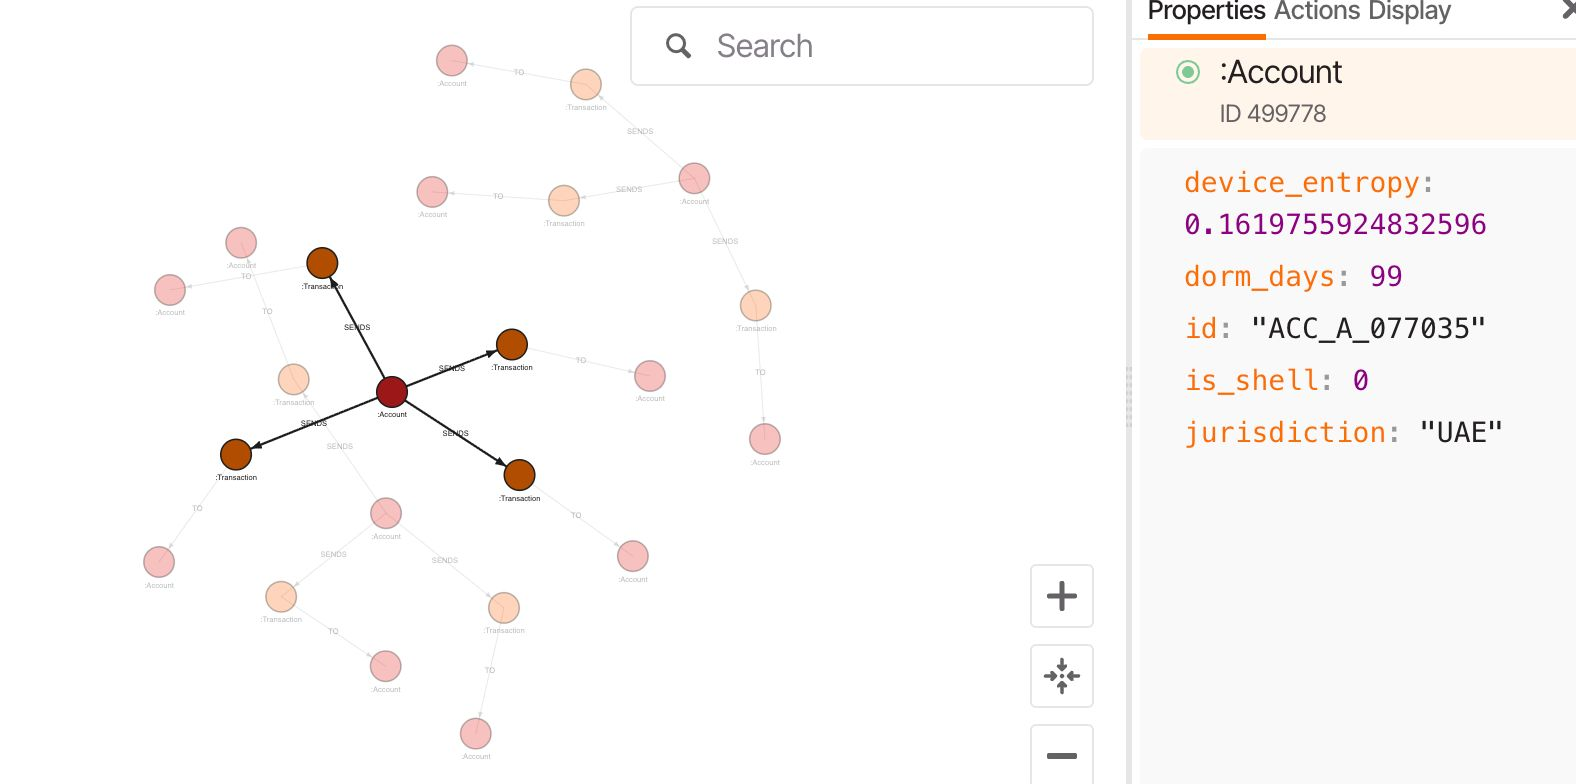
\includegraphics[width=0.95\textwidth]{Figures/memgraphlab.png}
    \caption{Heterogeneous financial transaction graph visualized within the Memgraph Lab environment.}
    \label{fig:memgraph_graph}
\end{figure}

%========================================================
\subsubsection[Hybrid HGNN--LSTM Analytical Implementation]{\textbf{Hybrid HGNN--LSTM Analytical Implementation}}
%========================================================

The proposed Hybrid HGNN--LSTM analytical module is implemented using PyTorch and PyTorch Geometric to perform graph-driven fraud analysis, temporal transaction modeling, and trade metadata learning for intelligent TBML detection. The implementation receives heterogeneous graph tensors generated from the Memgraph environment, including KYC node attributes, transactional edge relationships, sequential SWIFT transaction records, and trade-deviation features before forwarding them into the analytical inference pipeline. By combining graph attention learning with temporal sequence analysis and trade-feature fusion, the framework is capable of capturing both structural and behavioral fraud patterns across interconnected financial transaction networks.

The graph-learning branch utilizes a three-layer \texttt{GATv2Conv} architecture with multi-head attention mechanisms to perform neighborhood aggregation and graph message passing across interconnected financial entities \cite{brody2022gatv2}. The implemented graph layers process KYC-related node attributes such as shell-company indicators, jurisdiction metadata, and dormant-account characteristics to generate enriched graph embeddings capable of exposing hidden intermediary relationships and suspicious transaction-routing behavior. ReLU activation functions and dropout regularization are integrated after each graph convolution layer to improve representation stability during federated training operations. The generated graph embeddings are then aggregated using \texttt{global\_mean\_pool()} and fused with sequential SWIFT transaction features before being processed through the LSTM branch for temporal anomaly detection and sequential transaction behavior modeling. The temporal branch captures repeated payment structures, abnormal transaction timing behavior, and cyclic financial movement patterns that are difficult to identify using standalone graph-learning approaches.

Trade-specific metadata such as price-deviation attributes and cargo weight-gap indicators are independently processed using multilayer perceptron operations consisting of fully connected layers, Layer Normalization, ReLU activations, and dropout regularization mechanisms. The generated graph embeddings, temporal sequence representations, and trade-feature vectors are fused within the final analytical layer before being forwarded into the dense classification module for fraud prediction. The final classification layer categorizes transactions into predefined classes including \texttt{CLEAN}, \texttt{WATCHLIST}, and \texttt{FRAUD}. Experimental evaluation demonstrated stable federated convergence and strong fraud-class Precision--Recall performance across distributed institutional datasets. The overall implementation workflow of the proposed Hybrid HGNN--LSTM analytical module is illustrated in Figure~\ref{fig:hgnn_impl}.

\begin{figure}[H]
\centering

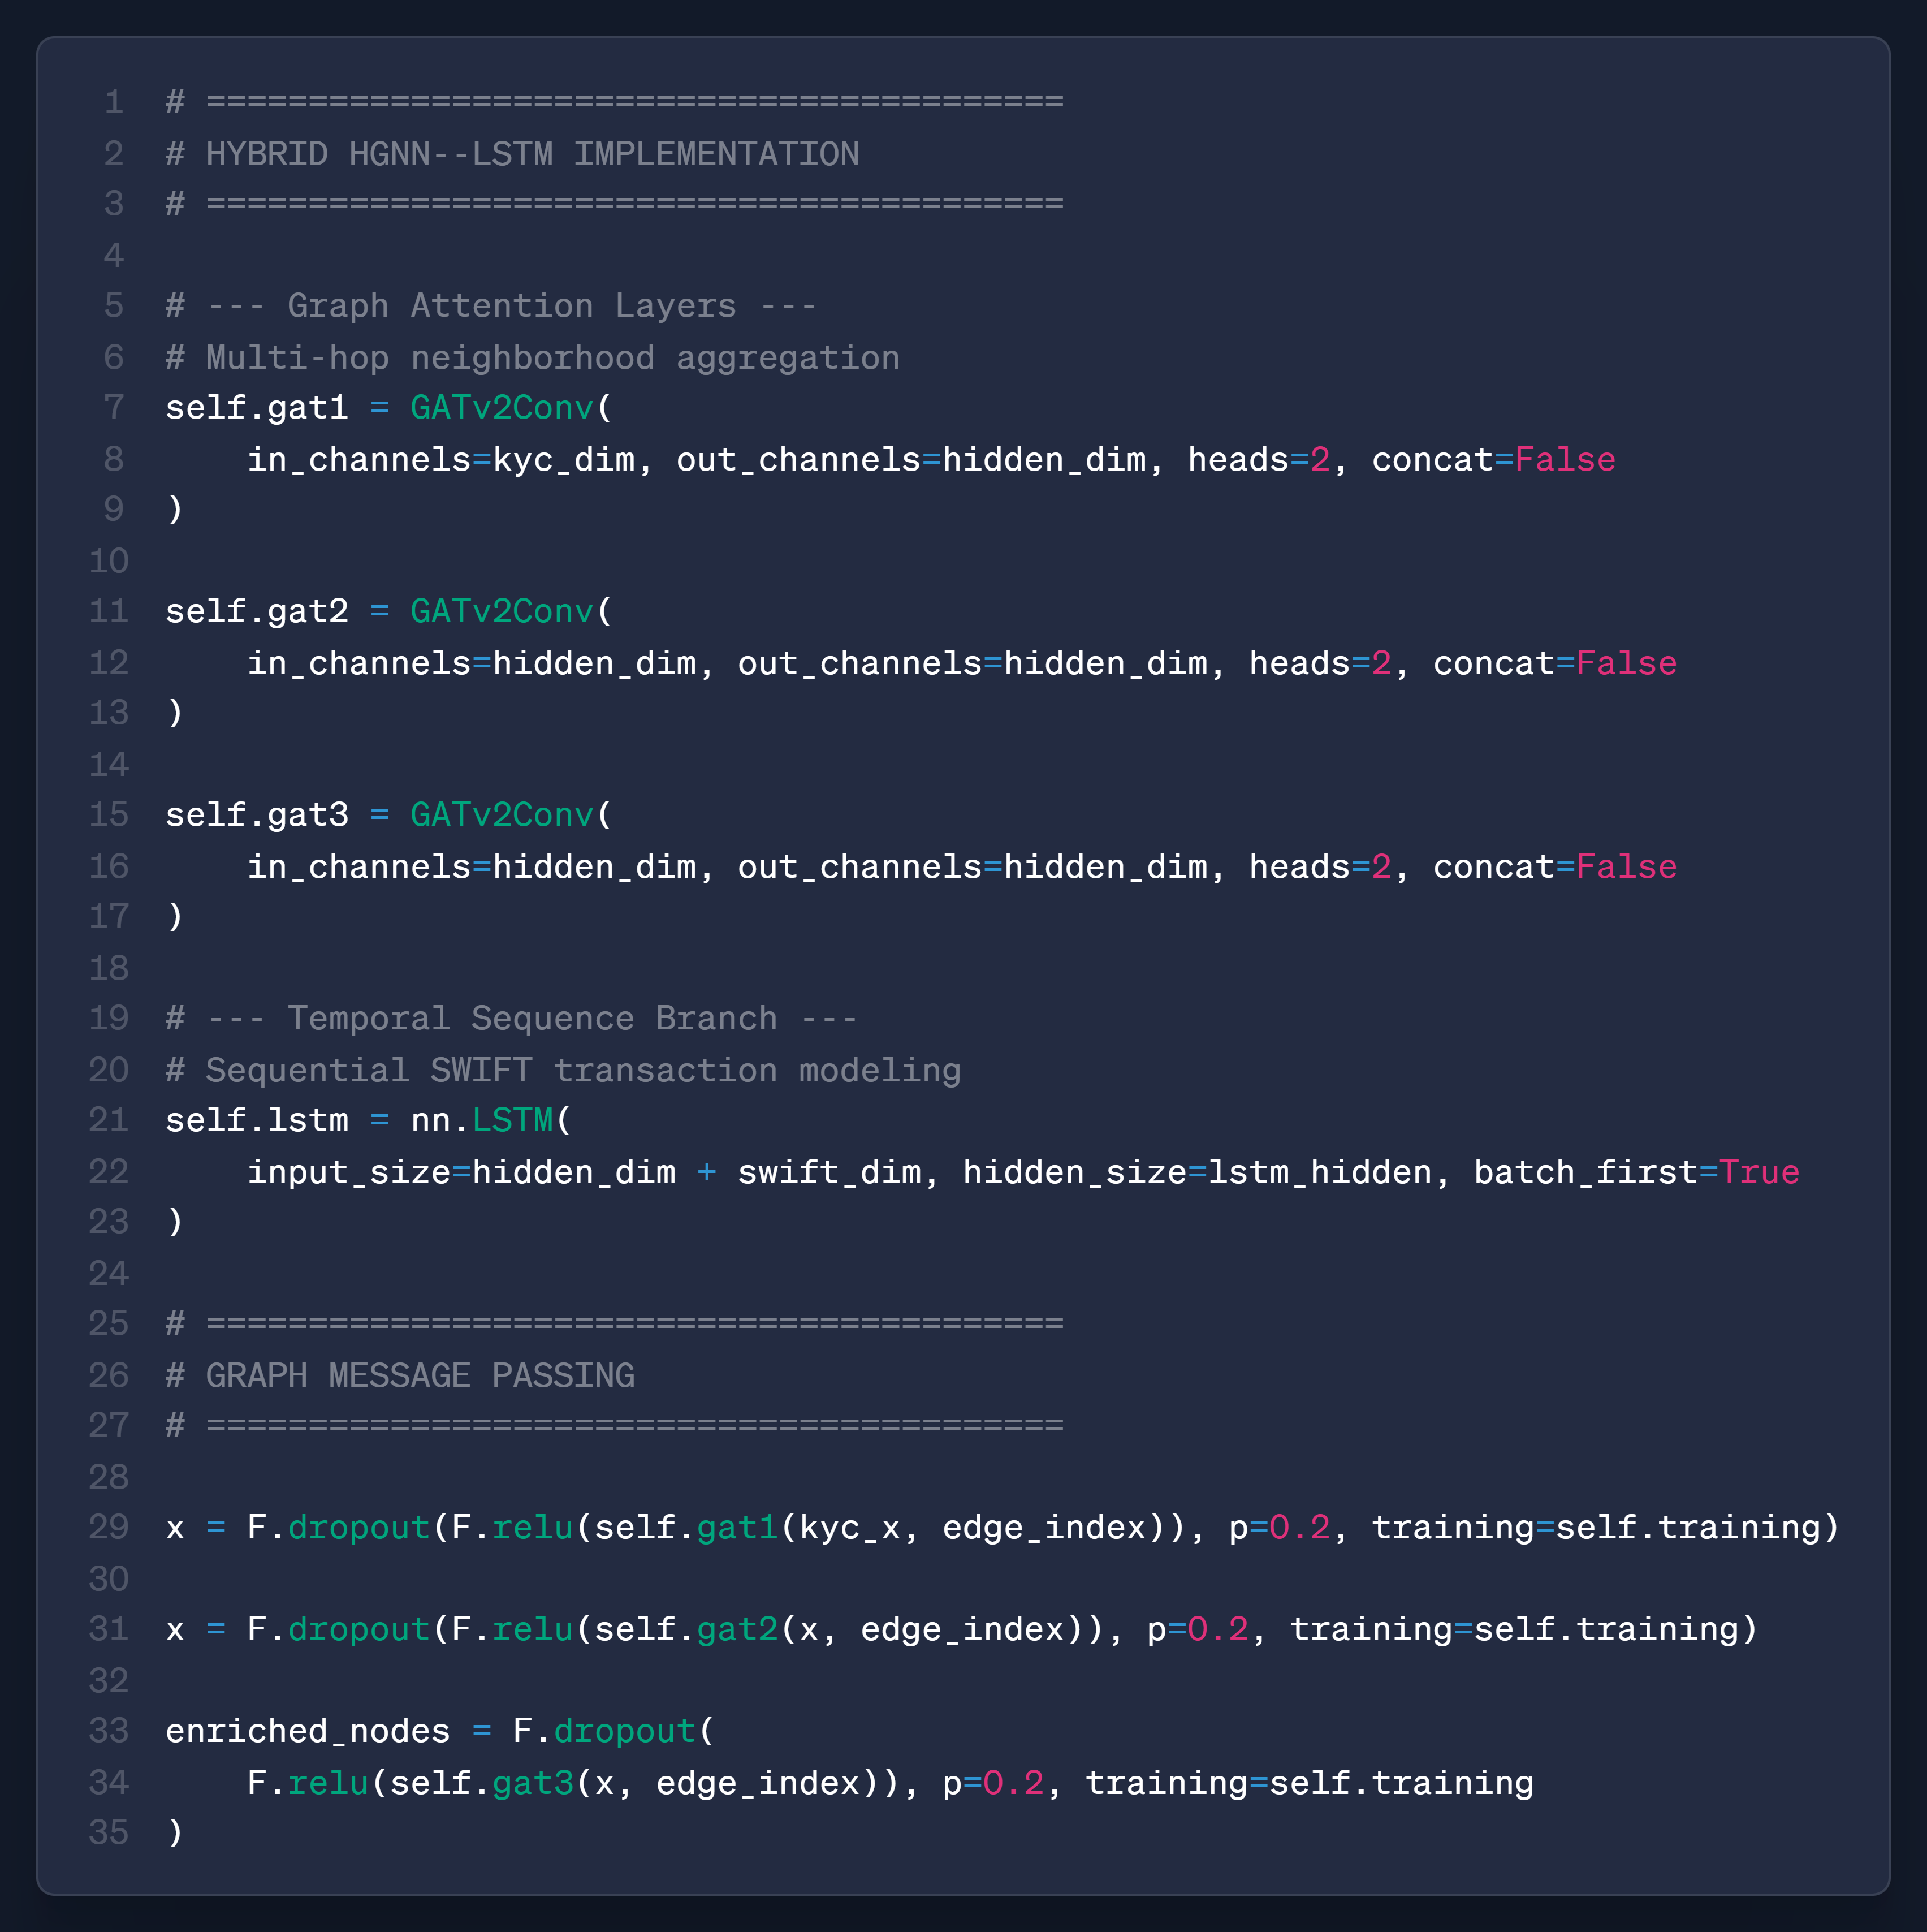
\includegraphics[width=0.48\textwidth]{Figures/model1.png}
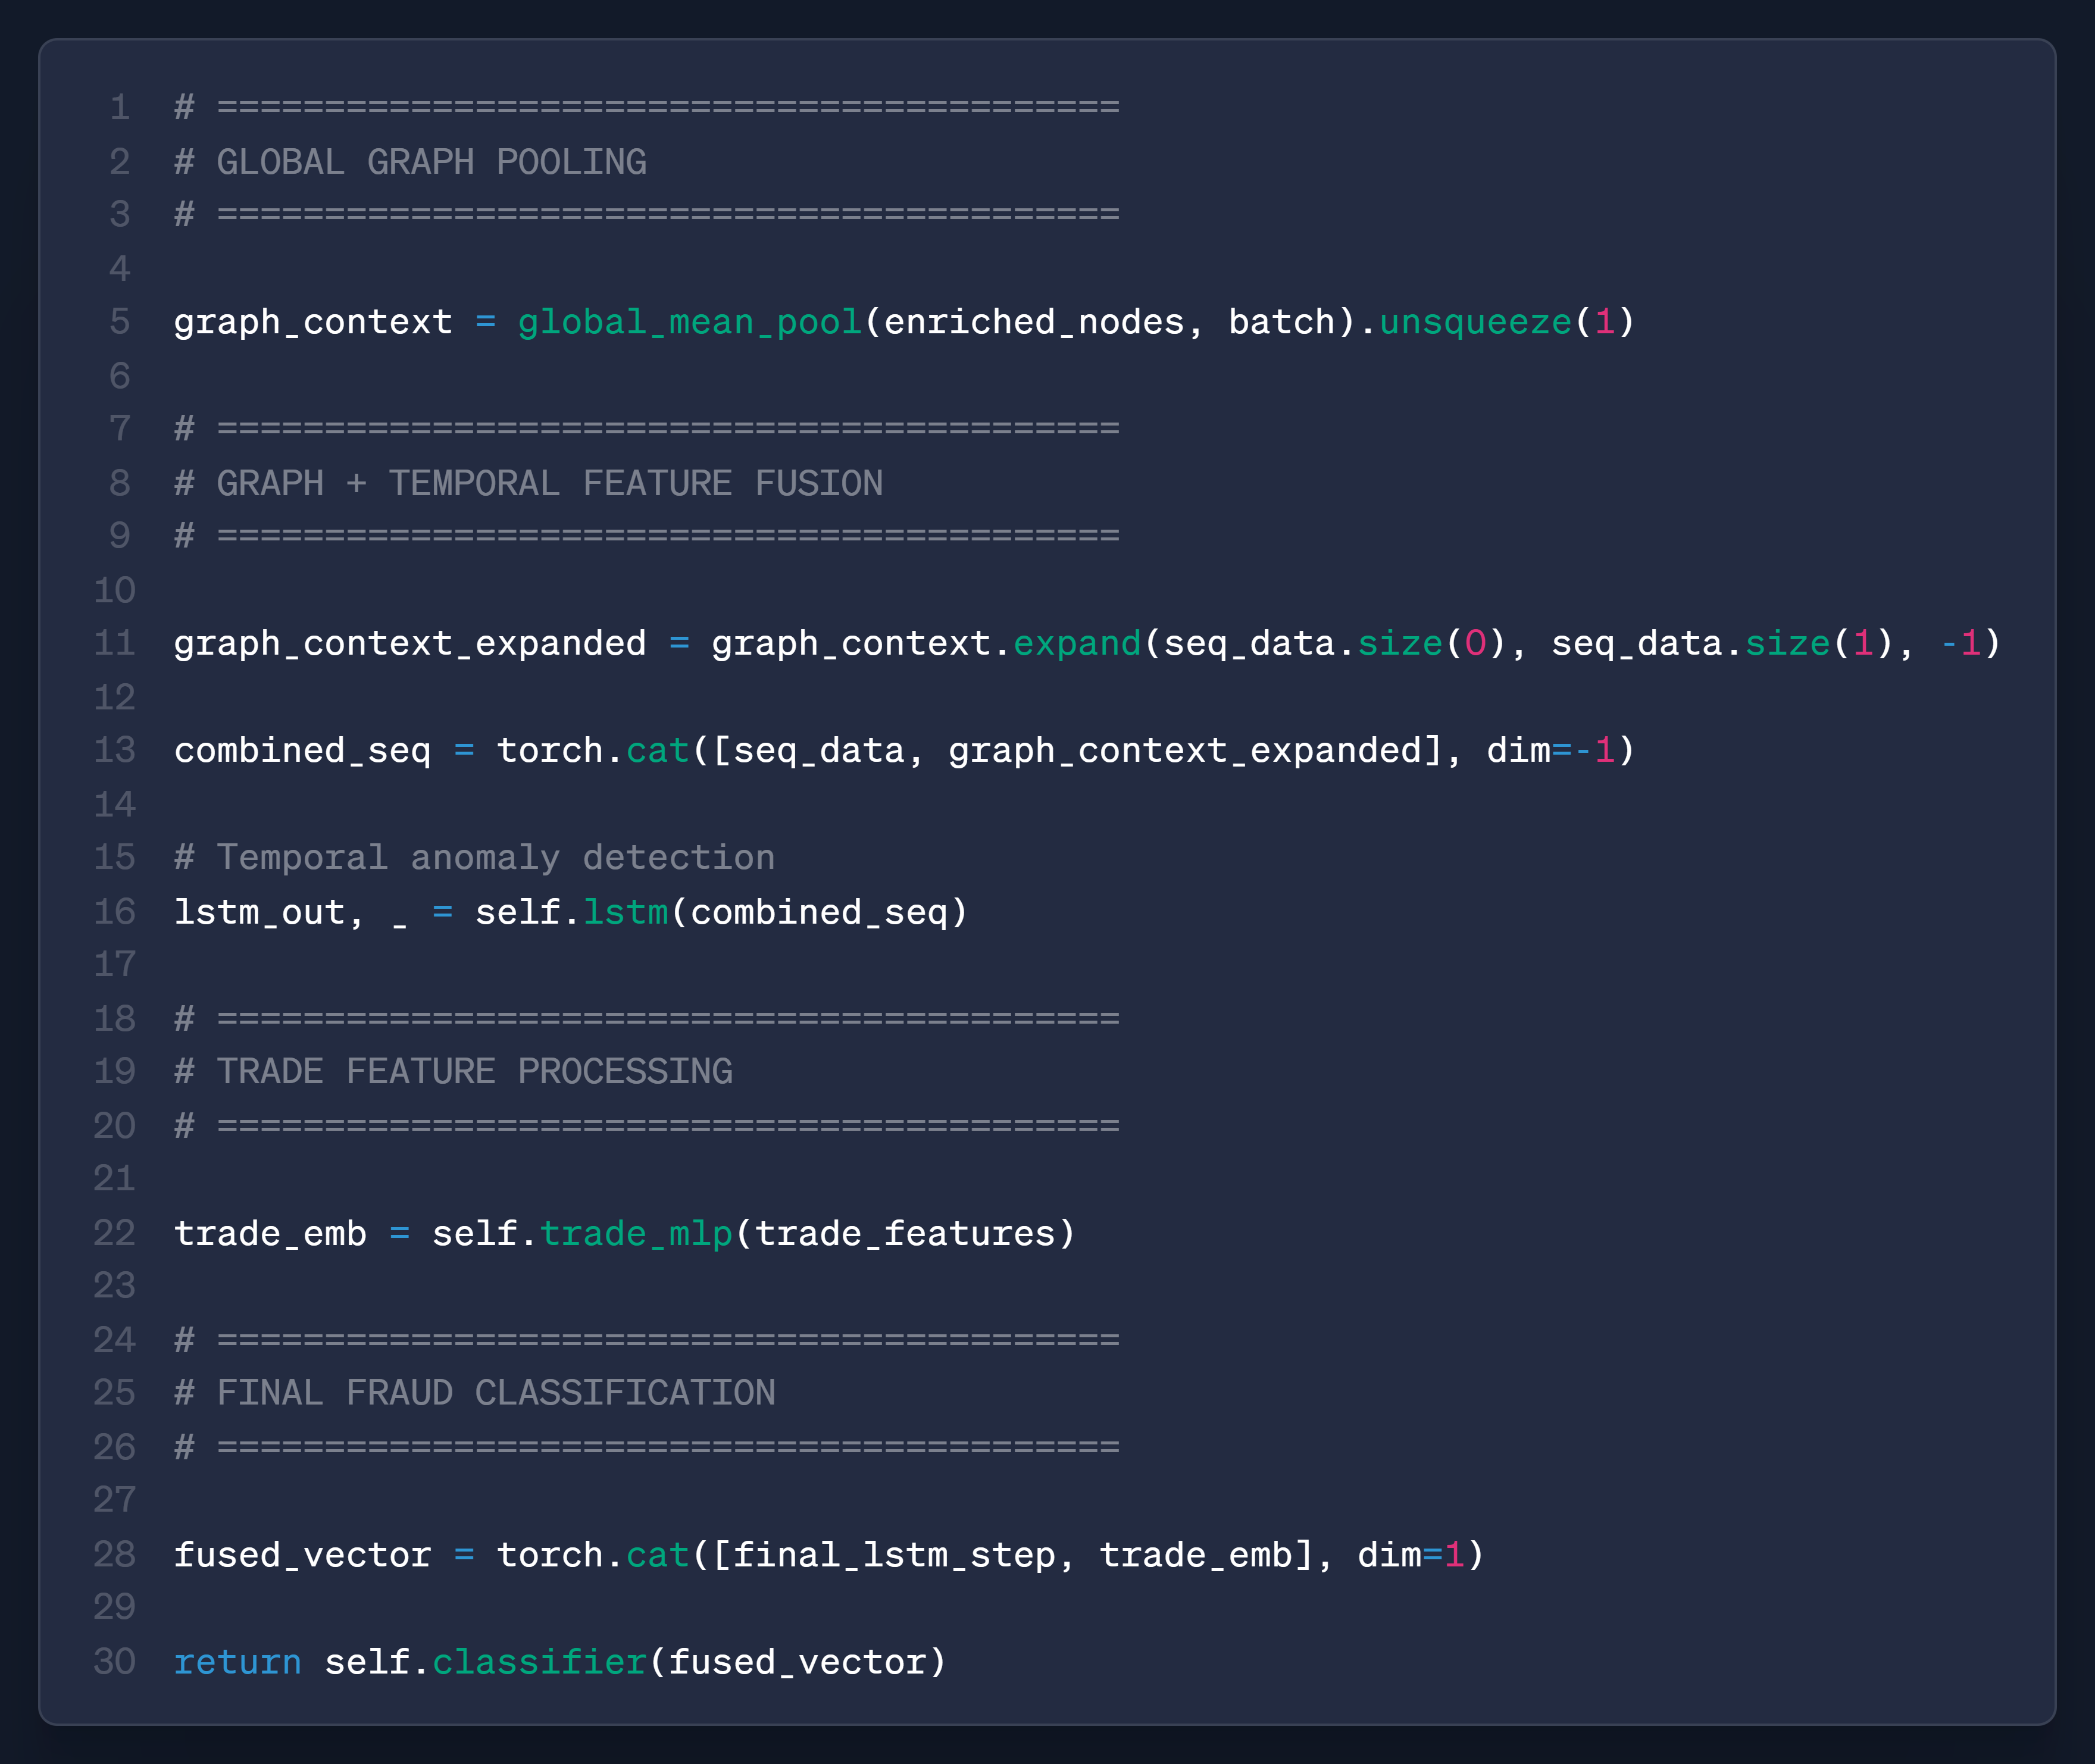
\includegraphics[width=0.48\textwidth]{Figures/model2.png}

\caption{Implementation workflow of the proposed Hybrid HGNN--LSTM analytical module.}

\label{fig:hgnn_impl}

\end{figure}


%========================================================
\subsubsection[Federated Learning Implementation]{\textbf{Federated Learning Implementation}}
%========================================================

The federated learning environment is implemented using the Flower federated learning framework to support distributed privacy-preserving fraud detection across multiple institutional clients. The implementation utilizes a centralized aggregation server and three participating institutional clients, where each client performs localized training of the proposed Hybrid HGNN--LSTM analytical model using institution-specific transaction graphs, sequential SWIFT transaction representations, and fraud classification labels without directly sharing sensitive financial records outside the local analytical environment.

The centralized aggregation server implements a custom federated strategy by extending the \texttt{flwr.server.strategy.FedAvg} class and overriding the \texttt{aggregate\_fit()} operation for distributed parameter aggregation. During each federated communication round, locally trained model weights generated from participating institutional clients are transmitted to the aggregation server where the \texttt{FedAvg} algorithm performs parameter averaging across synchronized client updates to generate a globally optimized fraud detection model. The server initializes the Hybrid HGNN--LSTM analytical architecture using synchronized feature dimensions including three-dimensional KYC node features, one-dimensional SWIFT transaction attributes, two-dimensional trade metadata features, hidden embedding dimensions of size 32, and three-class fraud prediction outputs.

The federated implementation performs ten synchronized communication rounds using complete client participation configurations including \texttt{fraction\_fit=1.0}, \texttt{min\_fit\_clients=3}, and \texttt{min\_available\_clients=3} to maintain stable distributed convergence across institutional environments \cite{kennedy2025federated}. After the final aggregation round, the globally optimized model parameters are converted from Flower parameter streams into NumPy tensors using \texttt{parameters\_to\_ndarrays()} before being serialized and stored as \texttt{global\_model.npz} for downstream real-time fraud inference operations. The implemented federated workflow enabled collaborative fraud learning, stable distributed convergence, and privacy-preserving analytical synchronization while maintaining complete institutional data isolation across participating financial organizations.


%========================================================
\subsection[User Interface and Compliance Workflow Implementation]{\textbf{User Interface and Compliance Workflow Implementation}}
%========================================================

The user interface and compliance-monitoring environment is implemented using Next.js, TypeScript, Tailwind CSS, Prisma ORM, Zustand state management, and PostgreSQL to support secure institutional fraud monitoring and centralized regulatory investigation workflows. The frontend architecture follows a modular service-oriented design consisting of protected dashboard routes, middleware-based authentication guards, API handlers, Prisma-powered database interaction layers, and role-specific monitoring interfaces integrated with the federated analytical inference environment.

%========================================================
\subsubsection[Authentication and Role Validation Pipeline]{\textbf{Authentication and Role Validation Pipeline}}
%========================================================

The authentication workflow is implemented using JWT-based session authorization combined with centralized middleware validation and protected route interception mechanisms. Incoming requests targeting protected dashboard routes are validated through middleware guards where session tokens are verified against predefined authorization scopes including \texttt{BANK\_ADMIN} and \texttt{REGULATOR}. Once validated, the session context is propagated across frontend environments through centralized authentication providers and Zustand-managed session states before protected dashboard components and compliance services are rendered within the client environment.

%========================================================
\subsubsection[Transaction Monitoring and Dashboard Rendering]{\textbf{Transaction Monitoring and Dashboard Rendering}}
%========================================================

Fraud predictions generated by the federated Hybrid HGNN--LSTM inference pipeline are synchronized into centralized PostgreSQL audit tables through backend transaction-processing services. Protected Next.js API handlers subsequently retrieve transaction classifications, fraud scores, STR metadata, and institutional monitoring information using Prisma query operations before dynamically rendering analytical outputs within role-specific dashboard interfaces. The banking administrator dashboard supports transaction filtering, fraud investigation workflows, watchlist escalation procedures, and false-positive reclassification operations through synchronized API-driven transaction state updates across centralized audit environments.

%========================================================
\subsubsection[STR Generation and Notification Workflow]{\textbf{STR Generation and Notification Workflow}}
%========================================================

Transactions classified as fraudulent trigger Suspicious Transaction Report (STR) generation workflows implemented through secured API endpoints and PostgreSQL-backed audit synchronization services. Institutional administrators initiate STR generation requests through protected dashboard interfaces where transaction metadata, fraud classifications, investigation summaries, institutional remarks, and compliance status information are serialized and stored within centralized STR audit tables. The generated STR records are subsequently propagated into regulator-facing monitoring environments through synchronized notification services and backend compliance-routing workflows.

%========================================================
\subsubsection[Regulatory Investigation and Compliance Monitoring]{\textbf{Regulatory Investigation and Compliance Monitoring}}
%========================================================

The regulatory monitoring environment consumes institution-generated STR records, fraud-classified transaction histories, compliance metadata, and supporting analytical evidence through protected API routes and Prisma-based database interaction layers. Regulatory authorities can perform investigation workflows including document-verification requests, institutional inquiry procedures, transaction review operations, and account-freeze initiation requests through centralized compliance interfaces synchronized with backend audit environments. The implemented monitoring workflow supports synchronized fraud prediction, institutional verification, STR lifecycle management, and centralized compliance monitoring within a unified real-time TBML analytical platform.


\section{Testing and Validation}
This section provides a comprehensive overview of the testing and validation processes employed to ensure the correctness, reliability, and performance of the proposed TBML detection framework. It includes descriptions of the testing environment, unit testing strategies for individual components, integration testing for end-to-end workflow validation, performance evaluation under simulated transaction loads, and security assessments to validate access control mechanisms and data protection measures within the framework.

%========================================================
\subsection[Testing Environment]{\textbf{Testing Environment}}
%========================================================

The testing process was conducted in a controlled development environment consisting of Python 3.11, PyTorch, PyTorch Geometric, Apache Kafka, Memgraph, PostgreSQL, and Flower federated learning services operating within isolated virtual environments created using \texttt{venv}. Frontend monitoring interfaces were implemented and validated using Next.js, TypeScript, Tailwind CSS, Prisma ORM, Zustand state management, and JWT-based authentication workflows.

The testing workflow additionally utilized Playwright-based browser automation for validating protected dashboard routes, institutional transaction workflows, STR generation pipelines, and compliance-monitoring interfaces. Database synchronization latency, transaction propagation consistency, backend API communication, and distributed fraud-inference workflows were validated under controlled institutional transaction loads to ensure reliable execution across distributed analytical environments.

%========================================================
\subsection[Unit Testing]{\textbf{Unit Testing}}
%========================================================

Each backend analytical service, dashboard workflow, authentication mechanism, and database synchronization component was independently tested to validate correctness, boundary handling, synchronization stability, and operational consistency before integration into the complete TBML detection framework.
%========================================================
\subsubsection[Unit Testing of Authentication and RBAC Module]{\textbf{Unit Testing of Authentication and RBAC Module}}
%========================================================

The authentication and role-based access control environment was independently validated to ensure secure user authentication, authorization management, middleware-driven route protection, credential verification, and institutional role isolation across banking and regulatory dashboard interfaces. The testing workflow additionally verified protected API access, invalid credential handling, unauthorized route restrictions, and role-specific dashboard rendering across distributed monitoring environments.
\renewcommand{\arraystretch}{1.3}

\begin{table}[H]
\centering
\caption{TC-001: Unit Testing of Authentication and RBAC Module}
\vspace{0.2cm}

\begin{tabular}{|p{4.2cm}|p{9cm}|}
\hline
\textbf{Serial Number of Test Case} & TC-001 \\ \hline
\textbf{Name of Test Case} & Protected Dashboard Access Validation \\ \hline
\textbf{Feature being Tested} & Authentication and Authorization Validation \\ \hline
\textbf{Description} & Validate protected route access, JWT verification, and role-based authorization \\ \hline
\textbf{Sample Input} & Invalid JWT session and unauthorized user request \\ \hline
\textbf{Expected Output} & Unauthorized access denied with authentication error response \\ \hline
\textbf{Actual Output} & Invalid sessions blocked and unauthorized users redirected successfully \\ \hline
\textbf{Remarks} & Successful test \\ \hline
\end{tabular}
\end{table}

Middleware-driven session validation successfully enforced protected route isolation and role-specific dashboard authorization across institutional monitoring environments. The testing workflow validated JWT token verification, session-expiration handling, credential validation, protected API access control, and middleware-based authorization checks across banking and regulator dashboards. Invalid credentials, unauthorized API requests, expired authentication sessions, and direct access attempts to protected routes were correctly rejected using backend access-control policies before protected resources were rendered. The authentication workflow additionally verified successful role mapping for \texttt{BANK\_USER} and  \texttt{ADMIN} entities to ensure secure dashboard isolation and controlled access to institutional fraud-monitoring operations.

%========================================================
\subsubsection[Unit Testing of Kafka Transaction Streaming]{\textbf{Unit Testing of Kafka Transaction Streaming}}
%========================================================

The Kafka transaction streaming environment was independently tested to validate asynchronous transaction publishing, real-time event synchronization, payload integrity validation, and downstream analytical communication across distributed backend services. The testing workflow additionally verified message delivery consistency, topic-based transaction propagation, malformed payload handling, and reliable synchronization between Kafka producer and consumer services operating within the proposed framework.


\begin{table}[H]
\centering
\caption{TC-002: Unit Testing of Kafka Transaction Streaming}
\vspace{0.2cm}

\begin{tabular}{|p{4.2cm}|p{9cm}|}
\hline
\textbf{Serial Number of Test Case} & TC-002 \\ \hline
\textbf{Name of Test Case} & Publish Valid SWIFT Transaction \\ \hline
\textbf{Feature being Tested} & Kafka Event Streaming and Message Synchronization \\ \hline
\textbf{Description} & Validate transaction publishing and topic-based event synchronization \\ \hline
\textbf{Sample Input} & JSON transaction payload containing sender, receiver, amount, and trade metadata \\ \hline
\textbf{Expected Output} & Transaction published into \texttt{incoming\_swift\_messages} topic successfully \\ \hline
\textbf{Actual Output} & Transaction streamed and synchronized successfully across Kafka services \\ \hline
\textbf{Remarks} & Successful test \\ \hline
\end{tabular}
\end{table}

The Kafka streaming module successfully validated asynchronous transaction publishing and backend event synchronization across distributed analytical services. Producer and consumer services maintained reliable message propagation and transaction consistency during continuous event-stream processing operations. Invalid payload structures, malformed transaction metadata, and incomplete financial events were correctly rejected through backend validation workflows before downstream graph-processing and fraud-inference operations were initiated.

%========================================================
\subsubsection[Unit Testing of Graph Construction Module]{\textbf{Unit Testing of Graph Construction Module}}
%========================================================

The heterogeneous graph-construction environment was independently tested to validate transactional node generation, relationship mapping, multi-entity graph synchronization, and Cypher-based ingestion workflows within the Memgraph analytical environment. The testing workflow additionally verified graph consistency, entity-link generation, transaction propagation accuracy, and downstream graph availability for Hybrid HGNN--LSTM analytical inference operations.

\begin{table}[H]
\centering
\caption{TC-003: Unit Testing of Graph Construction Module}
\vspace{0.2cm}

\begin{tabular}{|p{4.2cm}|p{9cm}|}
\hline
\textbf{Serial Number of Test Case} & TC-003 \\ \hline
\textbf{Name of Test Case} & Heterogeneous Graph Entity Generation \\ \hline
\textbf{Feature being Tested} & Memgraph Graph Construction and Relationship Mapping \\ \hline
\textbf{Description} & Validate transactional node generation and graph relationship synchronization \\ \hline
\textbf{Sample Input} & Valid SWIFT transaction payload with account, trade, and document metadata \\ \hline
\textbf{Expected Output} & Graph nodes and transactional relationships created successfully within Memgraph \\ \hline
\textbf{Actual Output} & Heterogeneous graph entities and multi-hop relationships generated successfully \\ \hline
\textbf{Remarks} & Successful test \\ \hline
\end{tabular}
\end{table}

The graph-construction workflow successfully generated heterogeneous transactional graphs within the Memgraph environment using Cypher-based ingestion and relationship-mapping operations. Graph entities including \texttt{(:Account)}, \texttt{(:Transaction)}, and \texttt{(:Document)} were correctly synchronized with transactional relationships such as \texttt{[:SENDS]}, \texttt{[:TO]}, and \texttt{[:HAS\_DOC]} during continuous event-stream processing. The testing workflow additionally validated graph consistency, entity-link integrity, and multi-hop transactional connectivity required for downstream subgraph extraction and graph-based fraud inference operations within the proposed framework.

%========================================================
\subsubsection[Unit Testing of STR Generation Workflow]{\textbf{Unit Testing of STR Generation Workflow}}
%========================================================

The STR generation workflow was independently tested to validate suspicious transaction report generation, compliance-record synchronization, fraud-case escalation, and regulator-side notification propagation across distributed institutional monitoring environments. The testing workflow additionally verified report persistence, transaction-metadata preservation, audit consistency, and downstream synchronization between banking dashboards and regulator-facing compliance interfaces.


\begin{table}[H]
\centering
\caption{TC-004: Unit Testing of STR Generation Workflow}
\vspace{0.2cm}

\begin{tabular}{|p{4.2cm}|p{9cm}|}
\hline
\textbf{Serial Number of Test Case} & TC-004 \\ \hline
\textbf{Name of Test Case} & Suspicious Transaction Report Generation \\ \hline
\textbf{Feature being Tested} & STR Generation and Compliance Synchronization \\ \hline
\textbf{Description} & Validate fraud escalation and regulator-side STR synchronization workflow \\ \hline
\textbf{Sample Input} & Fraud-classified transaction selected from institutional monitoring dashboard \\ \hline
\textbf{Expected Output} & STR record generated and synchronized into regulator compliance environment \\ \hline
\textbf{Actual Output} & STR generated, persisted, and synchronized successfully across monitoring services \\ \hline
\textbf{Remarks} & Successful test \\ \hline
\end{tabular}
\end{table}


The STR workflow successfully validated automated fraud-report generation, PostgreSQL audit synchronization, and regulator-side notification propagation across distributed institutional environments. Generated STR records correctly preserved transaction metadata, fraud classifications, institutional identifiers, and investigation references during downstream compliance synchronization operations. The testing workflow additionally verified successful dashboard synchronization, report persistence, and controlled propagation of suspicious transaction alerts between banking institutions and regulatory monitoring interfaces operating within the proposed framework.

%========================================================
\subsubsection[Unit Testing of Notification Workflow]{\textbf{Unit Testing of Notification Workflow}}
%========================================================

The notification synchronization environment was independently tested to validate fraud-alert propagation, institutional notification delivery, compliance-event synchronization, and regulator-side alert visibility across distributed monitoring interfaces. The testing workflow additionally verified notification persistence, dashboard update consistency, backend event propagation, and synchronization between banking and regulatory compliance environments during fraud escalation operations.


\begin{table}[H]
\centering
\caption{TC-005: Unit Testing of Notification Workflow}
\vspace{0.2cm}

\begin{tabular}{|p{4.2cm}|p{9cm}|}
\hline
\textbf{Serial Number of Test Case} & TC-005 \\ \hline
\textbf{Name of Test Case} & Fraud Alert and Compliance Notification Propagation \\ \hline
\textbf{Feature being Tested} & Notification Synchronization and Alert Delivery \\ \hline
\textbf{Description} & Validate fraud-alert propagation across banking and regulator monitoring environments \\ \hline
\textbf{Sample Input} & Generated STR record linked to fraud-classified transaction \\ \hline
\textbf{Expected Output} & Compliance alerts synchronized into regulator-facing dashboard interfaces \\ \hline
\textbf{Actual Output} & Fraud notifications propagated and synchronized successfully \\ \hline
\textbf{Remarks} & Successful test \\ \hline
\end{tabular}
\end{table}


The notification workflow successfully validated fraud-alert propagation, institutional investigation updates, and STR lifecycle synchronization across distributed compliance-monitoring environments. Backend event-processing services maintained reliable notification delivery and dashboard synchronization during fraud escalation operations between banking institutions and regulatory authorities. The testing workflow additionally verified notification persistence, regulator-side alert visibility, and consistent compliance-state propagation across protected monitoring interfaces operating within the proposed framework.



%========================================================
\subsection[Integration Testing]{\textbf{Integration Testing}}
%========================================================

Integration testing was conducted to validate the interaction, synchronization consistency, and workflow stability between distributed analytical services, graph-processing environments, fraud inference pipelines, dashboard-rendering systems, and regulatory compliance workflows operating within the proposed TBML detection framework.

%========================================================
\subsubsection[Integration Testing of Kafka and Memgraph Pipeline]{\textbf{Integration Testing of Kafka and Memgraph Pipeline}}
%========================================================

This integration test validated end-to-end synchronization between Kafka-based transaction streaming services and the heterogeneous graph-construction environment operating within Memgraph. The testing workflow additionally verified event-stream consistency, transaction propagation reliability, graph-ingestion stability, and downstream synchronization between distributed backend services.

\renewcommand{\arraystretch}{1.3}

\begin{table}[H]
\centering
\caption{TC-006: Integration Testing of Kafka and Memgraph Pipeline}
\vspace{0.2cm}

\begin{tabular}{|p{4.2cm}|p{9cm}|}
\hline
\textbf{Serial Number of Test Case} & TC-006 \\ \hline
\textbf{Name of Test Case} & Transaction Stream and Graph Synchronization Workflow \\ \hline
\textbf{Feature being Tested} & Kafka Event Propagation and Memgraph Synchronization \\ \hline
\textbf{Description} & Validate transaction-stream synchronization and heterogeneous graph generation \\ \hline
\textbf{Sample Input} & Valid Kafka transaction payload with trade metadata and KYC attributes \\ \hline
\textbf{Expected Output} & Transactional graph entities and relationships generated successfully within Memgraph \\ \hline
\textbf{Actual Output} & Kafka events synchronized and heterogeneous graph generated successfully \\ \hline
\textbf{Remarks} & Successful test \\ \hline
\end{tabular}
\end{table}

\renewcommand{\arraystretch}{1}

The integration workflow successfully validated asynchronous transaction propagation between Kafka producer-consumer services and Memgraph graph-ingestion environments. Streamed SWIFT transaction events were reliably synchronized into graph-processing pipelines without transactional inconsistency or event-loss during continuous backend processing operations. The testing workflow additionally verified stable graph synchronization, multi-entity relationship generation, and downstream availability of transactional subgraphs required for graph-based analytical inference within the proposed framework.


%========================================================
\subsubsection[Integration Testing of Fraud Prediction and Dashboard Synchronization]{\textbf{Integration Testing of Fraud Prediction and Dashboard Synchronization}}
%========================================================

This integration test checked how well the fraud-prediction services, PostgreSQL audit layer, and role-based monitoring dashboards worked together within the proposed TBML framework. It also confirmed that transaction results were stored correctly, updated reliably on the dashboard, and rendered in real time for fraud-monitoring review.

\renewcommand{\arraystretch}{1.3}

\begin{table}[H]
\centering
\caption{TC-007: Integration Testing of Fraud Prediction and Dashboard Synchronization}
\vspace{0.2cm}

\begin{tabular}{|p{4.2cm}|p{9cm}|}
\hline
\textbf{Serial Number of Test Case} & TC-007 \\ \hline
\textbf{Name of Test Case} & Fraud Prediction and Dashboard Rendering Workflow \\ \hline
\textbf{Feature being Tested} & PostgreSQL Synchronization and Dashboard Visualization \\ \hline
\textbf{Description} & Validate fraud-prediction synchronization into institutional monitoring dashboards \\ \hline
\textbf{Sample Input} & Fraud-classified transaction generated from analytical inference pipeline \\ \hline
\textbf{Expected Output} & Fraud transaction persisted and rendered successfully within dashboard interfaces \\ \hline
\textbf{Actual Output} & Dashboard synchronization completed successfully with valid fraud-state rendering \\ \hline
\textbf{Remarks} & Successful test \\ \hline
\end{tabular}
\end{table}

\renewcommand{\arraystretch}{1}

Fraud-prediction records, transaction metadata, and institutional risk classifications were synced into the central PostgreSQL audit environment and then displayed through protected dashboard interfaces. The dashboard updates stayed consistent across institutional monitoring services, giving users a clear real-time view of transaction status and fraud outcomes. The test also confirmed stable backend persistence, reliable dashboard refreshes, and secure rendering of fraud-monitoring data for each role-based compliance environment.

%========================================================
\subsubsection[Integration Testing of STR Generation Workflow]{\textbf{Integration Testing of STR Generation Workflow}}
%========================================================

This integration test covered the full path from institutional fraud review to STR generation, regulator synchronization, and compliance notifications across distributed monitoring environments. It verified that fraud escalation behaved consistently, reports were stored correctly, and regulators could see the same case information across their compliance pipelines.

The STR workflow worked as expected: once a transaction was marked for escalation, the system generated the compliance report, synchronized it to the regulator-side dashboard, and propagated the related notifications across the monitoring environment. Each STR record retained the key fraud classification details, investigation notes, institutional identifiers, and audit references needed for downstream compliance processing. The test also confirmed that compliance alerts reached the relevant banking and regulatory interfaces in a synchronized way.

\renewcommand{\arraystretch}{1.3}

\begin{table}[H]
\centering
\caption{TC-008: Integration Testing of STR Generation Workflow}
\vspace{0.2cm}

\begin{tabular}{|p{4.2cm}|p{9cm}|}
\hline
\textbf{Serial Number of Test Case} & TC-008 \\ \hline
\textbf{Name of Test Case} & Fraud Escalation and STR Compliance Workflow \\ \hline
\textbf{Feature being Tested} & STR Lifecycle Management and Compliance Synchronization \\ \hline
\textbf{Description} & Validate fraud escalation and regulator-side STR synchronization workflow \\ \hline
\textbf{Sample Input} & Fraud transaction escalated by institutional administrator \\ \hline
\textbf{Expected Output} & STR generated and synchronized successfully within regulator compliance dashboard \\ \hline
\textbf{Actual Output} & Fraud escalation and STR synchronization completed successfully \\ \hline
\textbf{Remarks} & Successful test \\ \hline
\end{tabular}
\end{table}

\renewcommand{\arraystretch}{1}


%========================================================
\subsubsection[Integration Testing of Authentication and Protected Dashboard Rendering]{\textbf{Integration Testing of Authentication and Protected Dashboard Rendering}}
%========================================================

This integration test validated synchronization between JWT-based authentication services, middleware-driven authorization guards, protected API routes, and role-specific dashboard-rendering environments operating within the proposed framework. The testing workflow additionally verified secure session propagation, authorization consistency, and protected resource accessibility across institutional monitoring interfaces.

Middleware-driven authentication workflows successfully validated session authorization, protected route synchronization, secure API accessibility, and institutional role isolation across distributed monitoring interfaces. Dashboard-rendering operations correctly enforced role-specific access-control policies for \texttt{BANK\_USER}, \texttt{ADMIN}, and \texttt{REGULATOR} entities during backend synchronization workflows. The testing workflow additionally verified invalid-session rejection, unauthorized route restrictions, and secure propagation of authenticated dashboard resources across institutional compliance-monitoring environments.
\renewcommand{\arraystretch}{1.3}

\begin{table}[H]
\centering
\caption{TC-009: Integration Testing of Authentication and Protected Dashboard Rendering}
\vspace{0.2cm}

\begin{tabular}{|p{4.2cm}|p{9cm}|}
\hline
\textbf{Serial Number of Test Case} & TC-009 \\ \hline
\textbf{Name of Test Case} & Authenticated Dashboard Access and Rendering Workflow \\ \hline
\textbf{Feature being Tested} & Session Validation and Role-Based Dashboard Authorization \\ \hline
\textbf{Description} & Validate authenticated dashboard rendering and protected route authorization \\ \hline
\textbf{Sample Input} & Valid JWT-authenticated institutional user session \\ \hline
\textbf{Expected Output} & Authorized dashboard rendered successfully based on institutional role \\ \hline
\textbf{Actual Output} & Protected dashboard rendered successfully with valid role authorization \\ \hline
\textbf{Remarks} & Successful test \\ \hline
\end{tabular}
\end{table}

\renewcommand{\arraystretch}{1}

%========================================================
\subsection[System Testing]{\textbf{System Testing}}
%========================================================

System testing was used to check how the proposed TBML detection framework behaved under realistic operational load. The focus was on end-to-end browser validation, protected dashboard execution, concurrent PostgreSQL access, API response times, and latency behavior across the fraud-monitoring and compliance-management services. The goal was to confirm that the system remained stable, responsive, and consistent when several components were active at the same time in a distributed institutional setting.

%========================================================
\subsubsection[Browser Automation and Workflow Validation]{\textbf{Browser Automation and Workflow Validation}}
%========================================================

Browser-based end-to-end validation was performed using Playwright automation workflows executed within Chromium testing environments. The testing workflow validated protected dashboard rendering, role-based authentication, STR lifecycle execution, fraud-notification propagation, compliance-action synchronization, and institutional transaction visibility restrictions across distributed frontend and backend services. All automated workflow executions completed successfully without unauthorized access, synchronization failure, or dashboard inconsistency during operational validation.

\renewcommand{\arraystretch}{1.3}

\begin{table}[H]
\centering
\caption{TC-010: Browser Automation and Workflow Validation Results}
\vspace{0.2cm}

\begin{tabular}{|p{7cm}|p{4cm}|}
\hline
\textbf{Workflow Validation} & \textbf{Status} \\ \hline
Admin Authentication and Dashboard Rendering & Successful \\ \hline
Fraud Case Retrieval and STR Visibility & Successful \\ \hline
GET\_DOCUMENTS Compliance Workflow & Successful \\ \hline
FREEZE\_ACCOUNT Regulatory Workflow & Successful \\ \hline
Fraud Verdict Marking Workflow & Successful \\ \hline
Bank User STR Generation Workflow & Successful \\ \hline
Fraud Notification Propagation Workflow & Successful \\ \hline
Protected Route and RBAC Validation & Successful \\ \hline
Institutional Transaction Visibility Restriction & Successful \\ \hline
Sign-In Page Smoke Testing & Successful \\ \hline
\end{tabular}
\end{table}

\renewcommand{\arraystretch}{1}

The Playwright automation workflow confirmed that institutional fraud-monitoring actions could be carried out in sequence across protected dashboard environments without interruption. It also verified secure session persistence, consistent API synchronization, proper workflow-level authorization, and stable dashboard rendering for both \texttt{ADMIN} and \texttt{BANK\_USER} users. In addition, the test showed that STR generation, fraud escalation, regulator-side compliance synchronization, and notification propagation all worked correctly in the automated end-to-end workflow.

%========================================================
\subsubsection[Concurrent Database Scalability and API Performance Analysis]{\textbf{Concurrent Database Scalability and API Performance Analysis}}
%========================================================

Concurrent database scalability testing assessed how well PostgreSQL synchronization held up under increasing institutional user loads, along with dashboard query performance, fraud-filtering latency, and STR retrieval consistency. The benchmark used Prisma ORM and Next.js backend services, and each simulated user sent five continuous transactional requests while accessing the dashboard. To keep the workload stable, the test used batched asynchronous requests, pooled PostgreSQL connections, and a limit of 15 active connections so that synchronization stayed reliable and backend resources were not overloaded during heavy monitoring activity.

Latency benchmarking was carried out by recording request-start and response-finish timestamps during concurrent API execution. For each request, the workflow captured the start time using \texttt{startTime = performance.now()}, sent the asynchronous API call, and then recorded the end time using \texttt{endTime = performance.now()} once the response returned. The latency was calculated as \texttt{latency = endTime - startTime}. The workload was run in parallel so that multiple simulated institutional users could issue dashboard and compliance queries at the same time under controlled concurrency limits.

Average latency reflected the mean response time across all successful requests, while P95 latency captured the slower end of the response distribution for 95\% of requests during peak load. The benchmark also checked request throughput, API synchronization consistency, transaction persistence reliability, and stable PostgreSQL query execution across distributed compliance-monitoring environments.

The benchmarking metrics were computed using the following operational latency equations:

\begin{equation}
L_{\text{avg}} =
\frac{1}{N}
\sum_{i=1}^{N}
(T_{\text{response}_i} - T_{\text{request}_i})
\end{equation}

\begin{equation}
L_{95} =
\operatorname{Percentile}_{95}(L_1, L_2, \dots, L_N)
\end{equation}

\renewcommand{\arraystretch}{1.3}

\begin{table}[H]
\centering
\caption{TC-011: Dashboard Transaction Retrieval Scalability Analysis}
\vspace{0.2cm}

\begin{tabular}{|p{2.6cm}|p{2.4cm}|p{2.8cm}|p{2.8cm}|p{2.2cm}|}
\hline
\textbf{Concurrent Users} & \textbf{Total Requests} & \textbf{Avg Latency (ms)} & \textbf{P95 Latency (ms)} & \textbf{Success Rate} \\ \hline
10 & 50 & 297.33 & 884.28 & 100\% \\ \hline
50 & 250 & 156.05 & 174.75 & 100\% \\ \hline
100 & 500 & 159.99 & 181.30 & 100\% \\ \hline
250 & 1250 & 158.53 & 176.99 & 100\% \\ \hline
500 & 2500 & 162.14 & 180.72 & 100\% \\ \hline
\end{tabular}
\end{table}

\renewcommand{\arraystretch}{1}

The dashboard transaction retrieval workflow demonstrated stable query scalability and consistent dashboard-rendering performance across increasing institutional user loads. Average latency values remained nearly constant between 50 and 500 concurrent users, indicating efficient PostgreSQL query execution, optimized transactional indexing, and stable backend synchronization during high-frequency dashboard-access operations. The relatively low variation between average and P95 latency measurements further indicated predictable response behavior and controlled query-execution overhead under concurrent transactional workloads.

\renewcommand{\arraystretch}{1.3}

\begin{table}[H]
\centering
\caption{TC-012: Fraud Transaction Filtering Scalability Analysis}
\vspace{0.2cm}

\begin{tabular}{|p{2.6cm}|p{2.4cm}|p{2.8cm}|p{2.8cm}|p{2.2cm}|}
\hline
\textbf{Concurrent Users} & \textbf{Total Requests} & \textbf{Avg Latency (ms)} & \textbf{P95 Latency (ms)} & \textbf{Success Rate} \\ \hline
10 & 50 & 159.58 & 174.04 & 100\% \\ \hline
50 & 250 & 158.15 & 181.58 & 100\% \\ \hline
100 & 500 & 147.56 & 170.37 & 100\% \\ \hline
250 & 1250 & 148.18 & 164.58 & 100\% \\ \hline
500 & 2500 & 263.80 & 731.88 & 100\% \\ \hline
\end{tabular}
\end{table}

\renewcommand{\arraystretch}{1}

The fraud-transaction filtering workflow demonstrated efficient analytical-query execution and stable institution-specific transaction retrieval during concurrent dashboard operations. Lower average latency values under moderate workloads indicated optimized fraud-state filtering and indexed transactional query execution across backend analytical services. Increased P95 latency under 500-user workloads indicated temporary synchronization overhead during peak concurrent analytical filtering operations; however, the framework maintained complete request reliability, stable API synchronization, and consistent fraud-state propagation throughout distributed monitoring workflows.

\renewcommand{\arraystretch}{1.3}

\begin{table}[H]
\centering
\caption{TC-013: STR Compliance Report Retrieval Scalability Analysis}
\vspace{0.2cm}

\begin{tabular}{|p{2.6cm}|p{2.4cm}|p{2.8cm}|p{2.8cm}|p{2.2cm}|}
\hline
\textbf{Concurrent Users} & \textbf{Total Requests} & \textbf{Avg Latency (ms)} & \textbf{P95 Latency (ms)} & \textbf{Success Rate} \\ \hline
10 & 50 & 2694.21 & 7311.50 & 100\% \\ \hline
50 & 250 & 2101.61 & 4791.52 & 100\% \\ \hline
100 & 500 & 856.39 & 2149.27 & 100\% \\ \hline
250 & 1250 & 467.03 & 600.67 & 100\% \\ \hline
500 & 2500 & 465.62 & 596.76 & 100\% \\ \hline
\end{tabular}
\end{table}

\renewcommand{\arraystretch}{1}

The STR compliance retrieval workflow showed higher latency than the other dashboard operations because it had to aggregate compliance reports, synchronize transaction history, retrieve regulator-side metadata, and execute several relational queries during report generation. Even so, the drop in average latency as concurrency increased suggested that PostgreSQL query handling became more stable, pooled connections were used more efficiently, and relational queries were executed more smoothly during sustained processing.

Although compliance-report generation added extra processing overhead, the framework still maintained consistent request behavior and a complete success rate across distributed monitoring environments. Overall, the testing workflows showed reliable backend synchronization, controlled API responses, stable federated analytical execution, and steady PostgreSQL performance as institutional workload increased.


Taken together, the testing results confirmed that the proposed TBML detection framework remained reliable, stable, and consistent across graph-processing, federated inference, dashboard synchronization, and compliance-management services. The scalability results also showed that PostgreSQL execution stayed stable and latency remained controlled even as institutional traffic increased.



%========================================================
\subsection[Model Performance Evaluation]{\textbf{Model Performance Evaluation}}
%========================================================

The proposed federated Hybrid HGNN--LSTM framework was evaluated across three distributed institutional clients (BANKA, BANKB, and BANKC) to validate fraud-classification capability and federated convergence stability across heterogeneous transactional environments. Multi-class prediction performance for \textit{Clean}, \textit{Watchlist}, and \textit{Fraud} transaction states was analyzed using Precision, Recall, F1-Score, confusion-matrix validation, and Precision--Recall benchmarking. Federated parameter synchronization was performed using the FedAvg aggregation strategy across 10 federated communication rounds.

The transactional dataset was partitioned using a stratified temporal split strategy to preserve chronological separation between training and testing samples while maintaining balanced representation across minority fraud categories. Weighted cross-entropy optimization and gradient clipping mechanisms were integrated to stabilize distributed training and address fraud-class imbalance during federated convergence operations. Precision--Recall evaluation was prioritized over standalone classification accuracy due to the highly imbalanced nature of illicit transactional behavior within institutional financial environments.

%========================================================
\subsubsection[Multi-Class Classification Performance]{\textbf{Multi-Class Classification Performance}}
%========================================================

The final federated classification results obtained after 10 federated aggregation rounds across all participating institutional environments are summarized in Table~\ref{tab:model_performance}. The evaluation was conducted to analyze the framework’s ability to distinguish legitimate, suspicious, and fraudulent transactional behaviors across distributed institutional datasets under federated learning conditions. The obtained results additionally validated stable analytical convergence and consistent fraud-classification performance across all participating banking clients.


The results showed that the model classified the three transaction states consistently across all institutional clients. Clean transactions were identified with near-perfect Precision and Recall, which helped keep false positives low during large-scale monitoring. The Watchlist class also performed well, with Recall remaining above $0.97$, showing that the model could reliably flag suspicious activity for institutional review.

\begin{table}[H]
\centering
\caption{Federated Multi-Class Classification Performance result}
\vspace{0.2cm}

\renewcommand{\arraystretch}{1.3}

\begin{tabular}{|p{2.2cm}|p{3cm}|p{2cm}|p{2cm}|p{2cm}|}
\hline
\textbf{Institution} & \textbf{Transaction Class} & \textbf{Precision} & \textbf{Recall} & \textbf{F1-Score} \\ \hline

\multirow{3}{*}{BANKA}
& Clean (0) & 1.00 & 1.00 & 1.00 \\ \cline{2-5}
& Watchlist (1) & 0.79 & 0.97 & 0.87 \\ \cline{2-5}
& Fraud (2) & 0.96 & 0.73 & 0.83 \\ \hline

\multirow{3}{*}{BANKB}
& Clean (0) & 1.00 & 1.00 & 1.00 \\ \cline{2-5}
& Watchlist (1) & 0.79 & 0.99 & 0.88 \\ \cline{2-5}
& Fraud (2) & 0.98 & 0.73 & 0.84 \\ \hline

\multirow{3}{*}{BANKC}
& Clean (0) & 1.00 & 1.00 & 1.00 \\ \cline{2-5}
& Watchlist (1) & 0.79 & 0.99 & 0.88 \\ \cline{2-5}
& Fraud (2) & 0.98 & 0.73 & 0.84 \\ \hline

\end{tabular}

\renewcommand{\arraystretch}{1}

\label{tab:model_performance}
\end{table}


Fraud-class predictions achieved Precision values between $0.96$ and $0.98$, which indicates that high-risk transactions were identified with very few false fraud alerts. Fraud Recall stayed around $0.73$, but the framework still preserved strong fraud-detection capability even with highly imbalanced data and complex multi-hop laundering structures. Overall, the results showed that the federated model generalized well across distributed institutions without requiring sensitive data to be centralized.


%========================================================
\subsubsection[Federated Convergence Analysis]{\textbf{Federated Convergence Analysis}}
%========================================================

Federated convergence was evaluated by tracking Accuracy, Precision, and Recall across successive aggregation rounds. Separate curves were generated for BANKA, BANKB, and BANKC so that the synchronization behavior of each institutional client could be observed independently. This made it possible to confirm that local updates were being aggregated correctly and that the global model was stabilizing as training progressed.

%--------------------------------------------------------
\subsubsection{BANKA Federated Convergence}
%--------------------------------------------------------

\begin{figure}[H]
\centering

\begin{minipage}{0.32\textwidth}
\centering
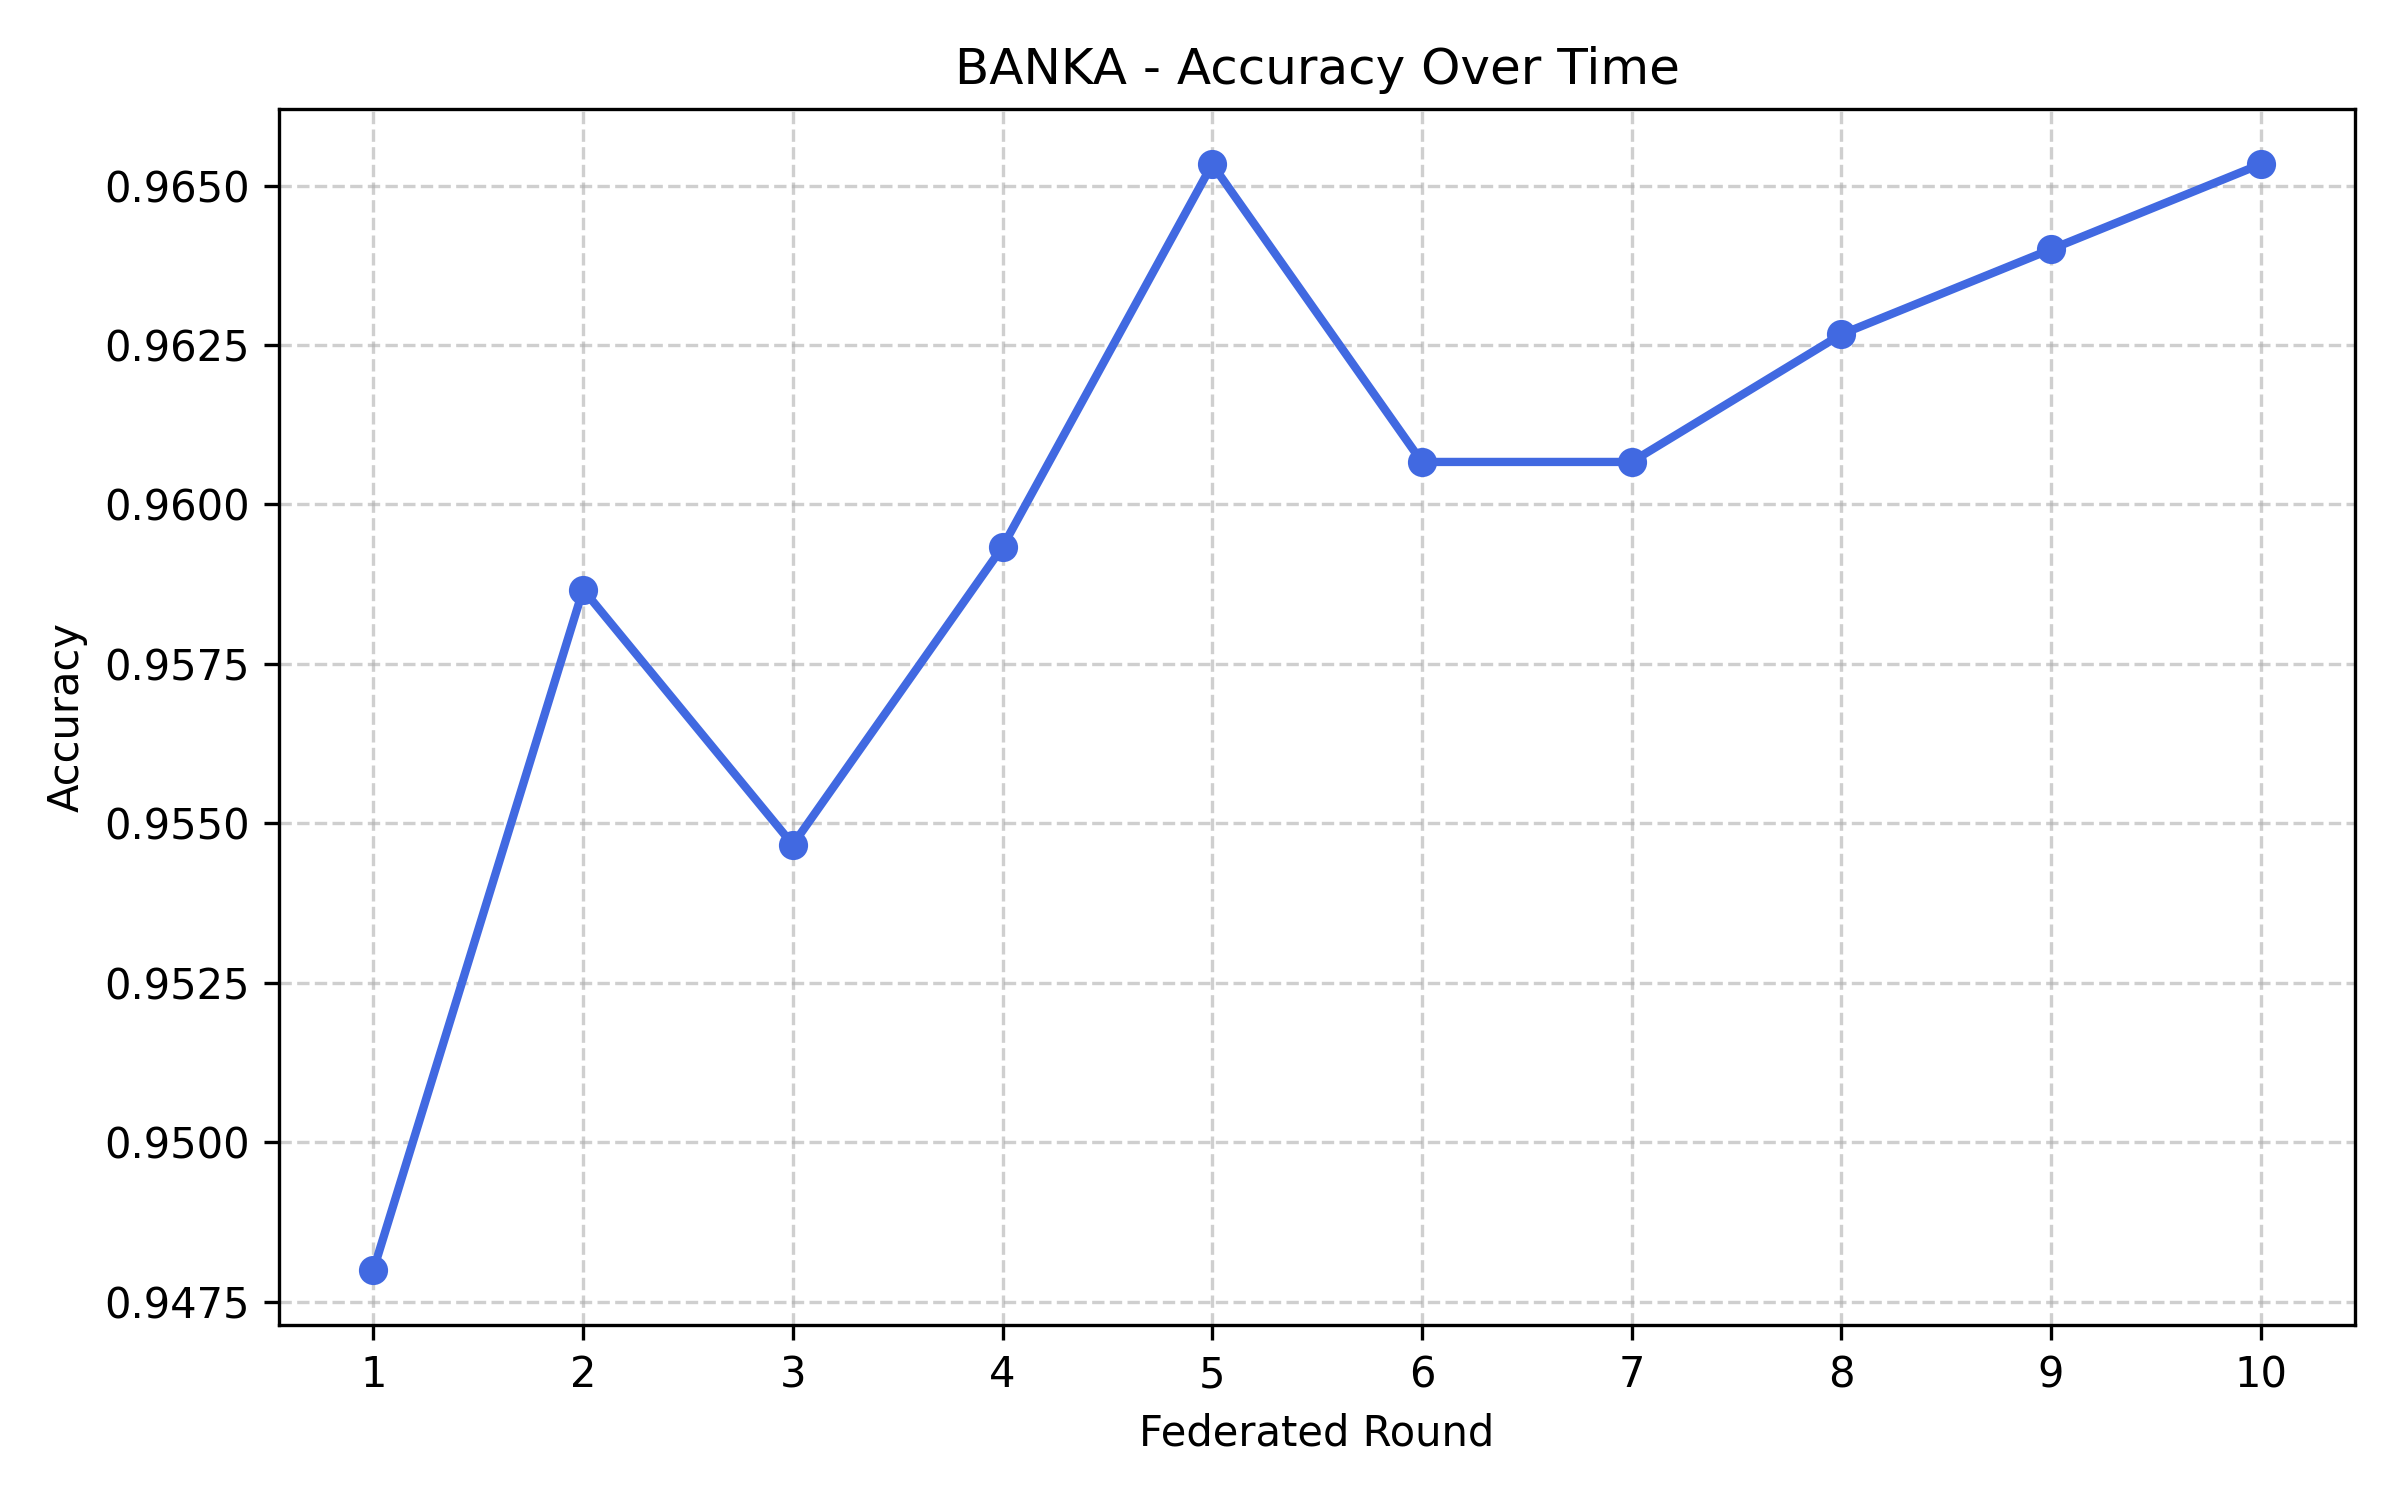
\includegraphics[width=\linewidth]{Figures/banka_progression_accuracy.png}
\end{minipage}
\hfill
\begin{minipage}{0.32\textwidth}
\centering
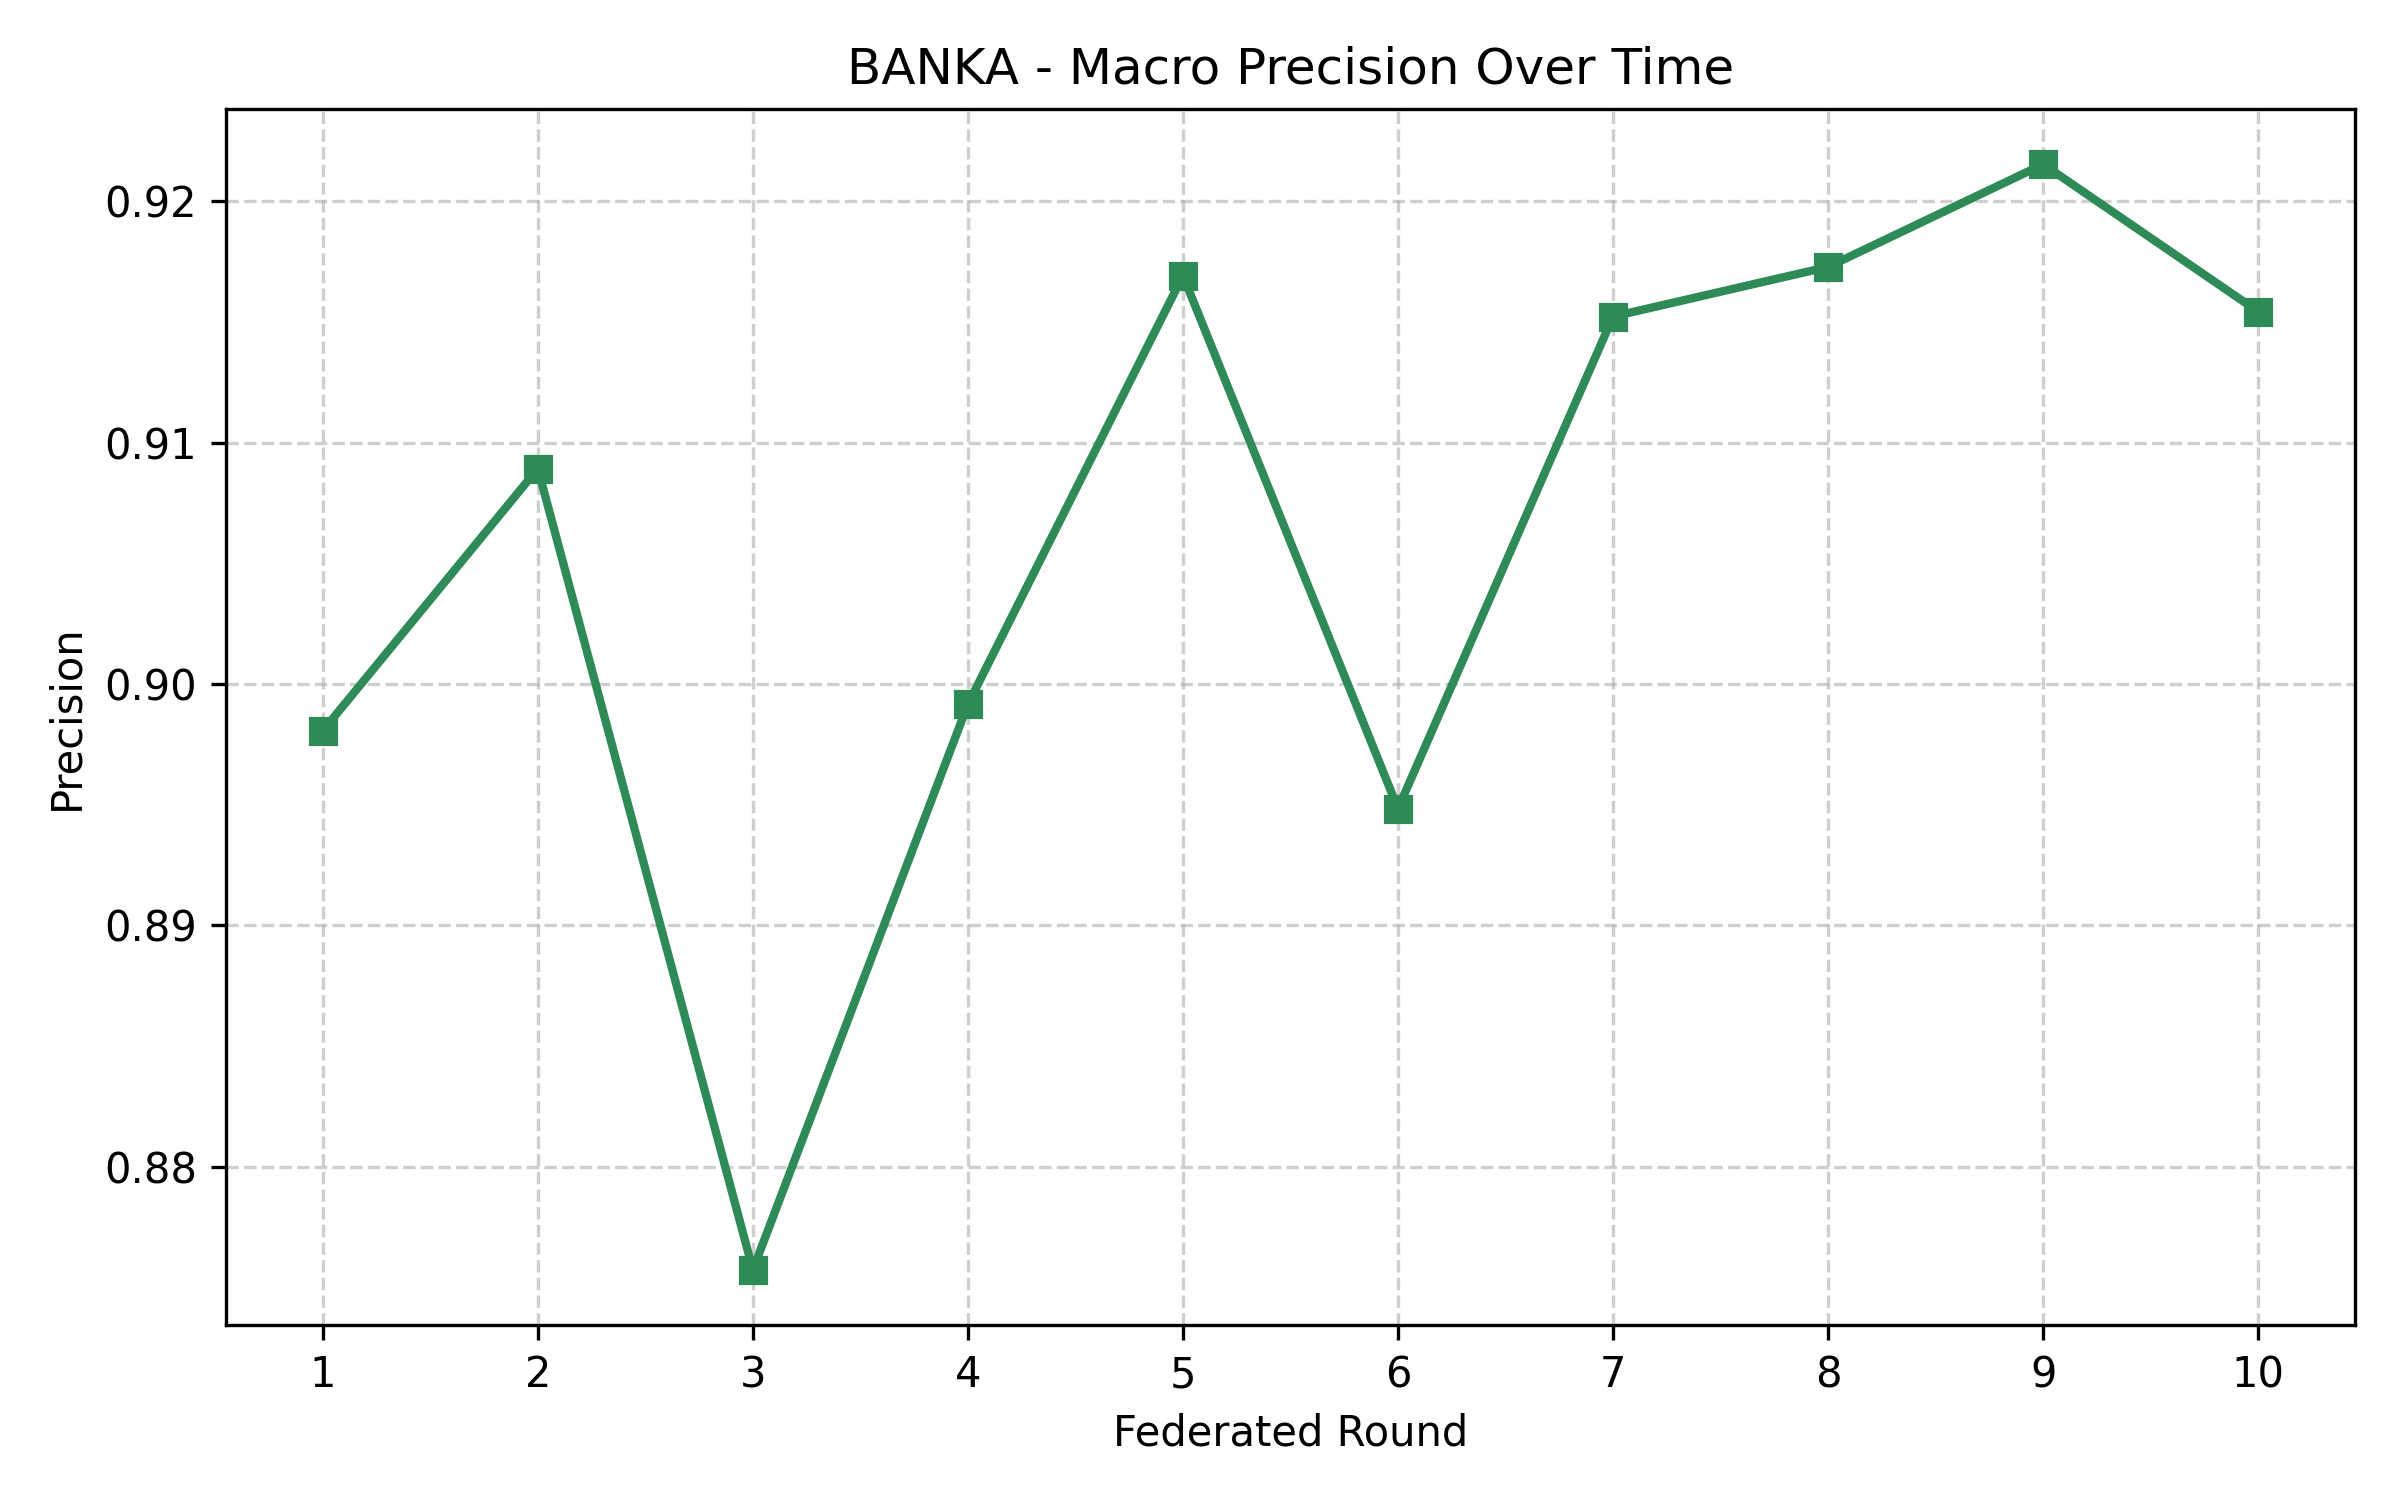
\includegraphics[width=\linewidth]{Figures/banka_progression_precision.png}
\end{minipage}
\hfill
\begin{minipage}{0.32\textwidth}
\centering
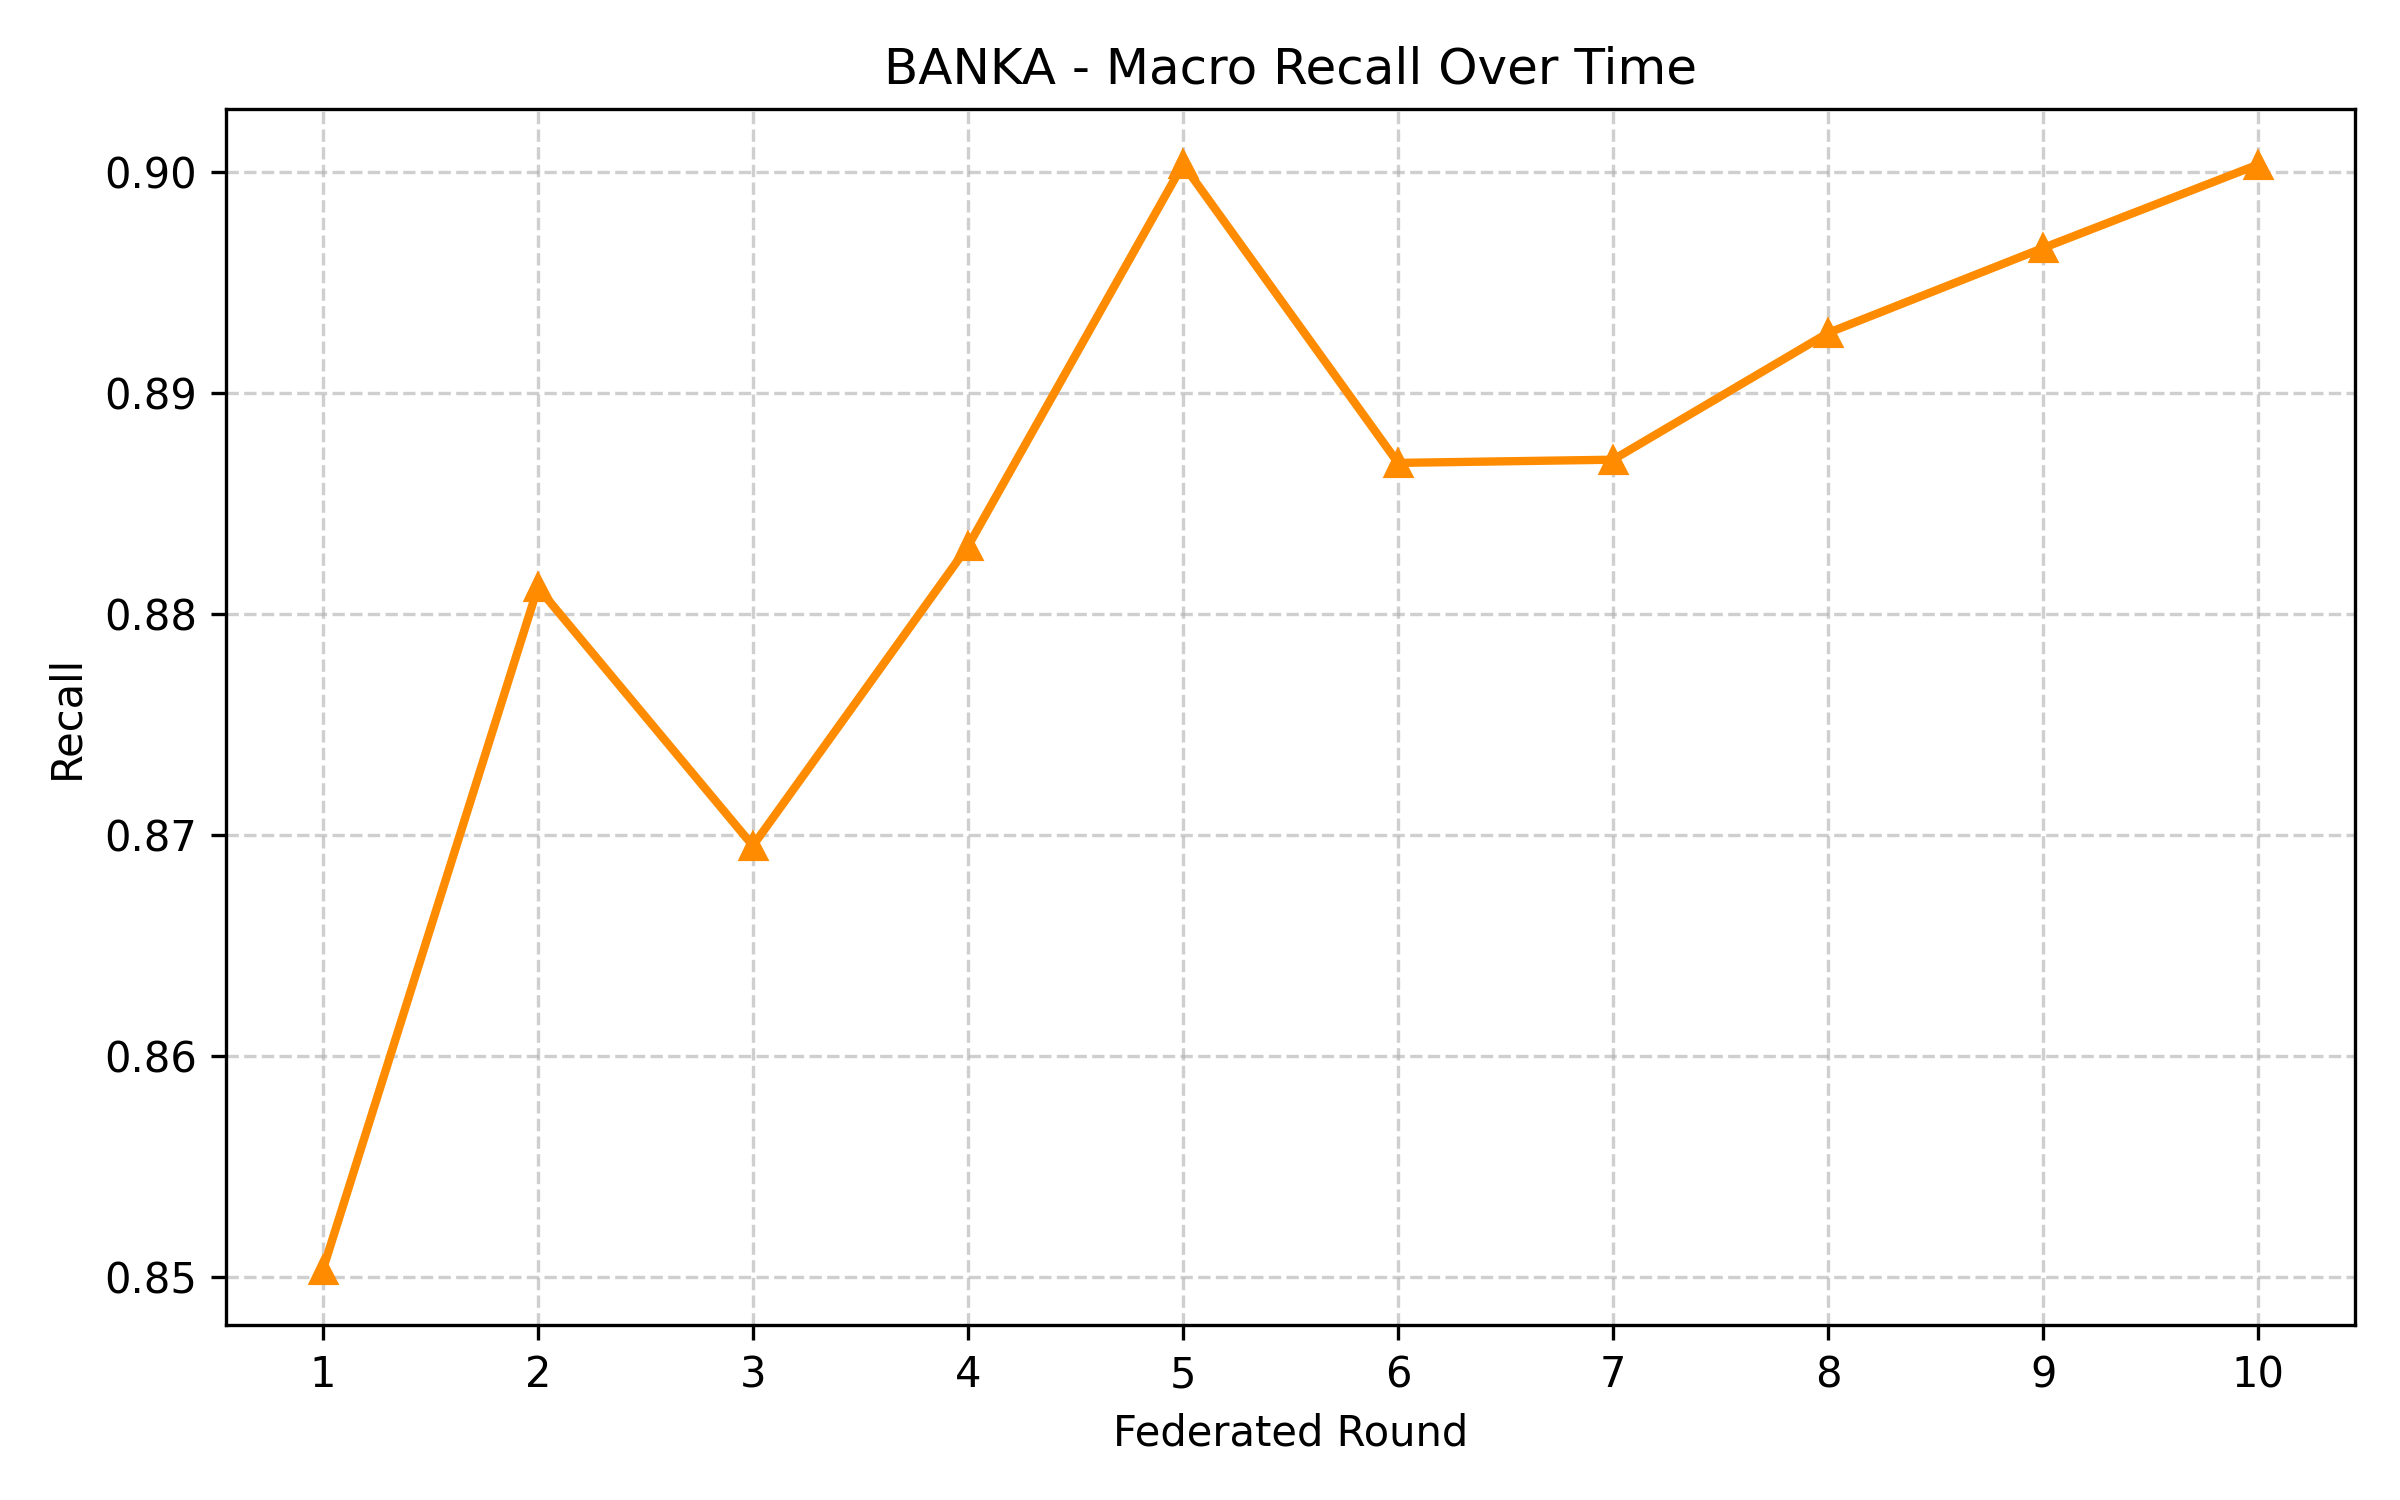
\includegraphics[width=\linewidth]{Figures/banka_progression_recall.png}
\end{minipage}

\caption{BANKA Federated Accuracy, Precision, and Recall Progression Across Federated Aggregation Rounds}
\label{fig:banka_progression}
\end{figure}

As shown in Figure~\ref{fig:banka_progression}, BANKA showed the expected training dynamics for a federated setup. The early variation was reduced as global aggregation and distributed weight synchronization started to dominate the optimization process, and the Accuracy, Precision, and Recall curves became noticeably smoother in the later rounds. That pattern indicates that the client was converging in a controlled way and that the federated updates were being integrated properly.
%--------------------------------------------------------
\subsubsection{BANKB Federated Convergence}
%--------------------------------------------------------

\begin{figure}[H]
\centering

\begin{minipage}{0.32\textwidth}
\centering
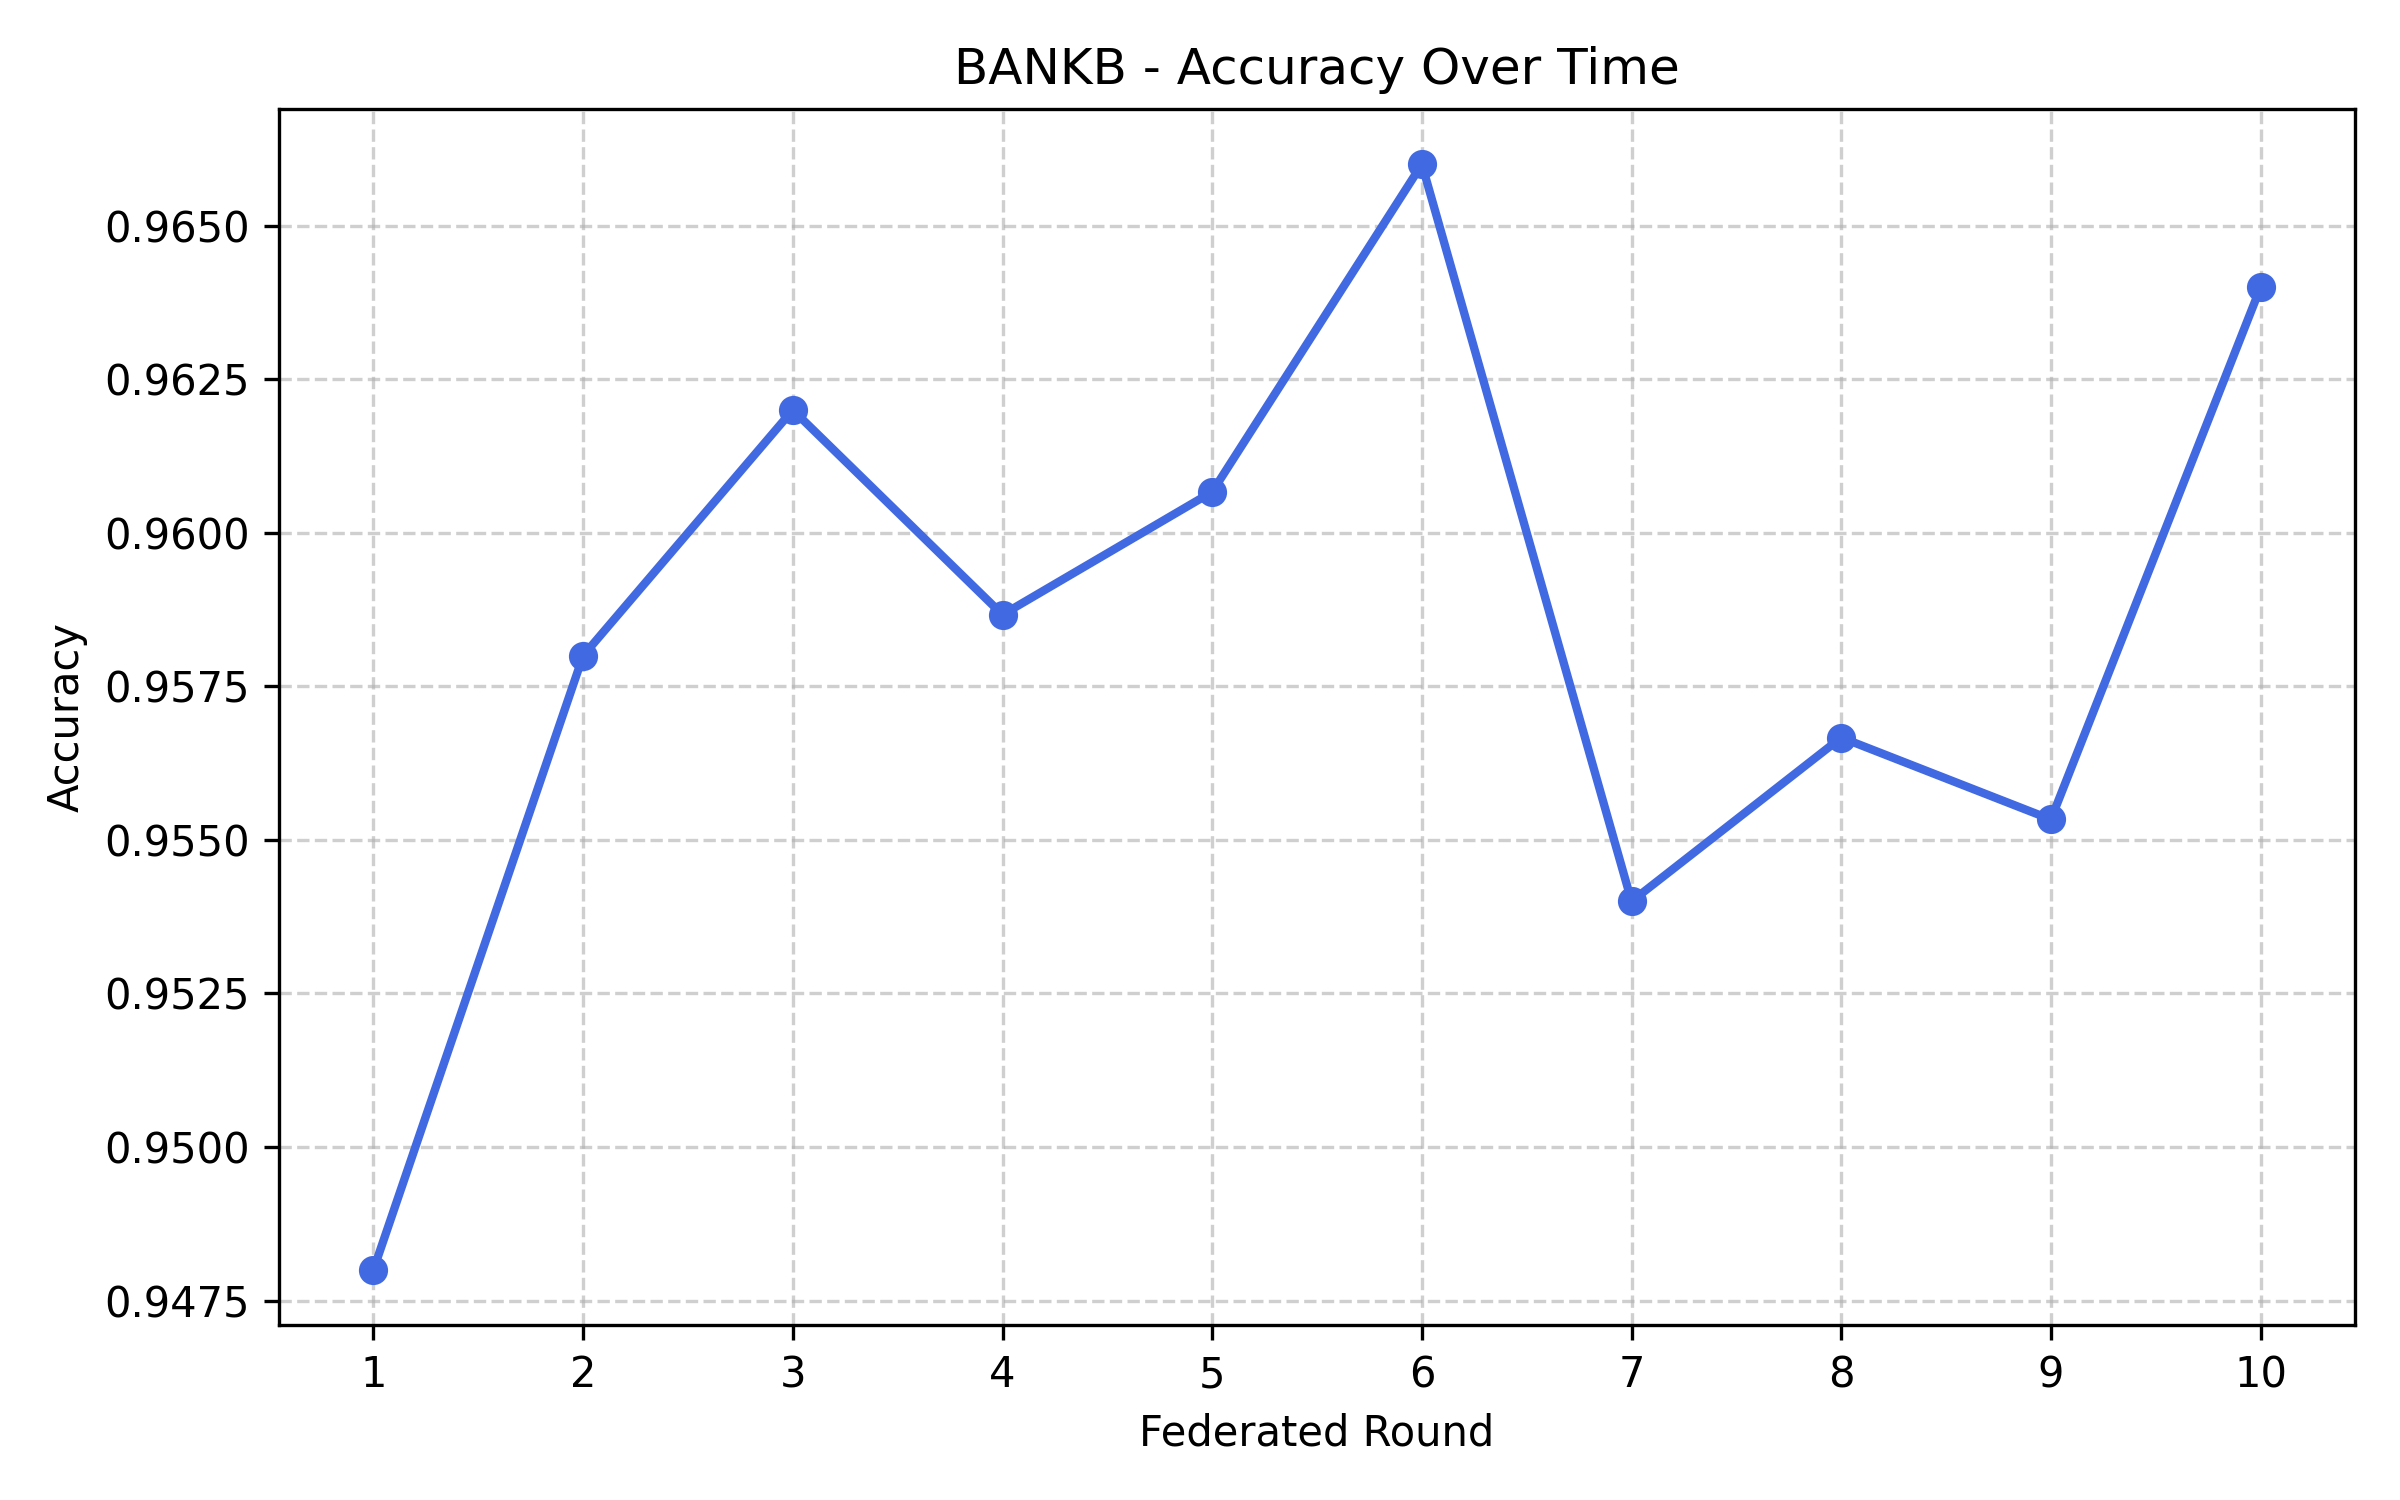
\includegraphics[width=\linewidth]{Figures/bankb_progression_accuracy.png}
\end{minipage}
\hfill
\begin{minipage}{0.32\textwidth}
\centering
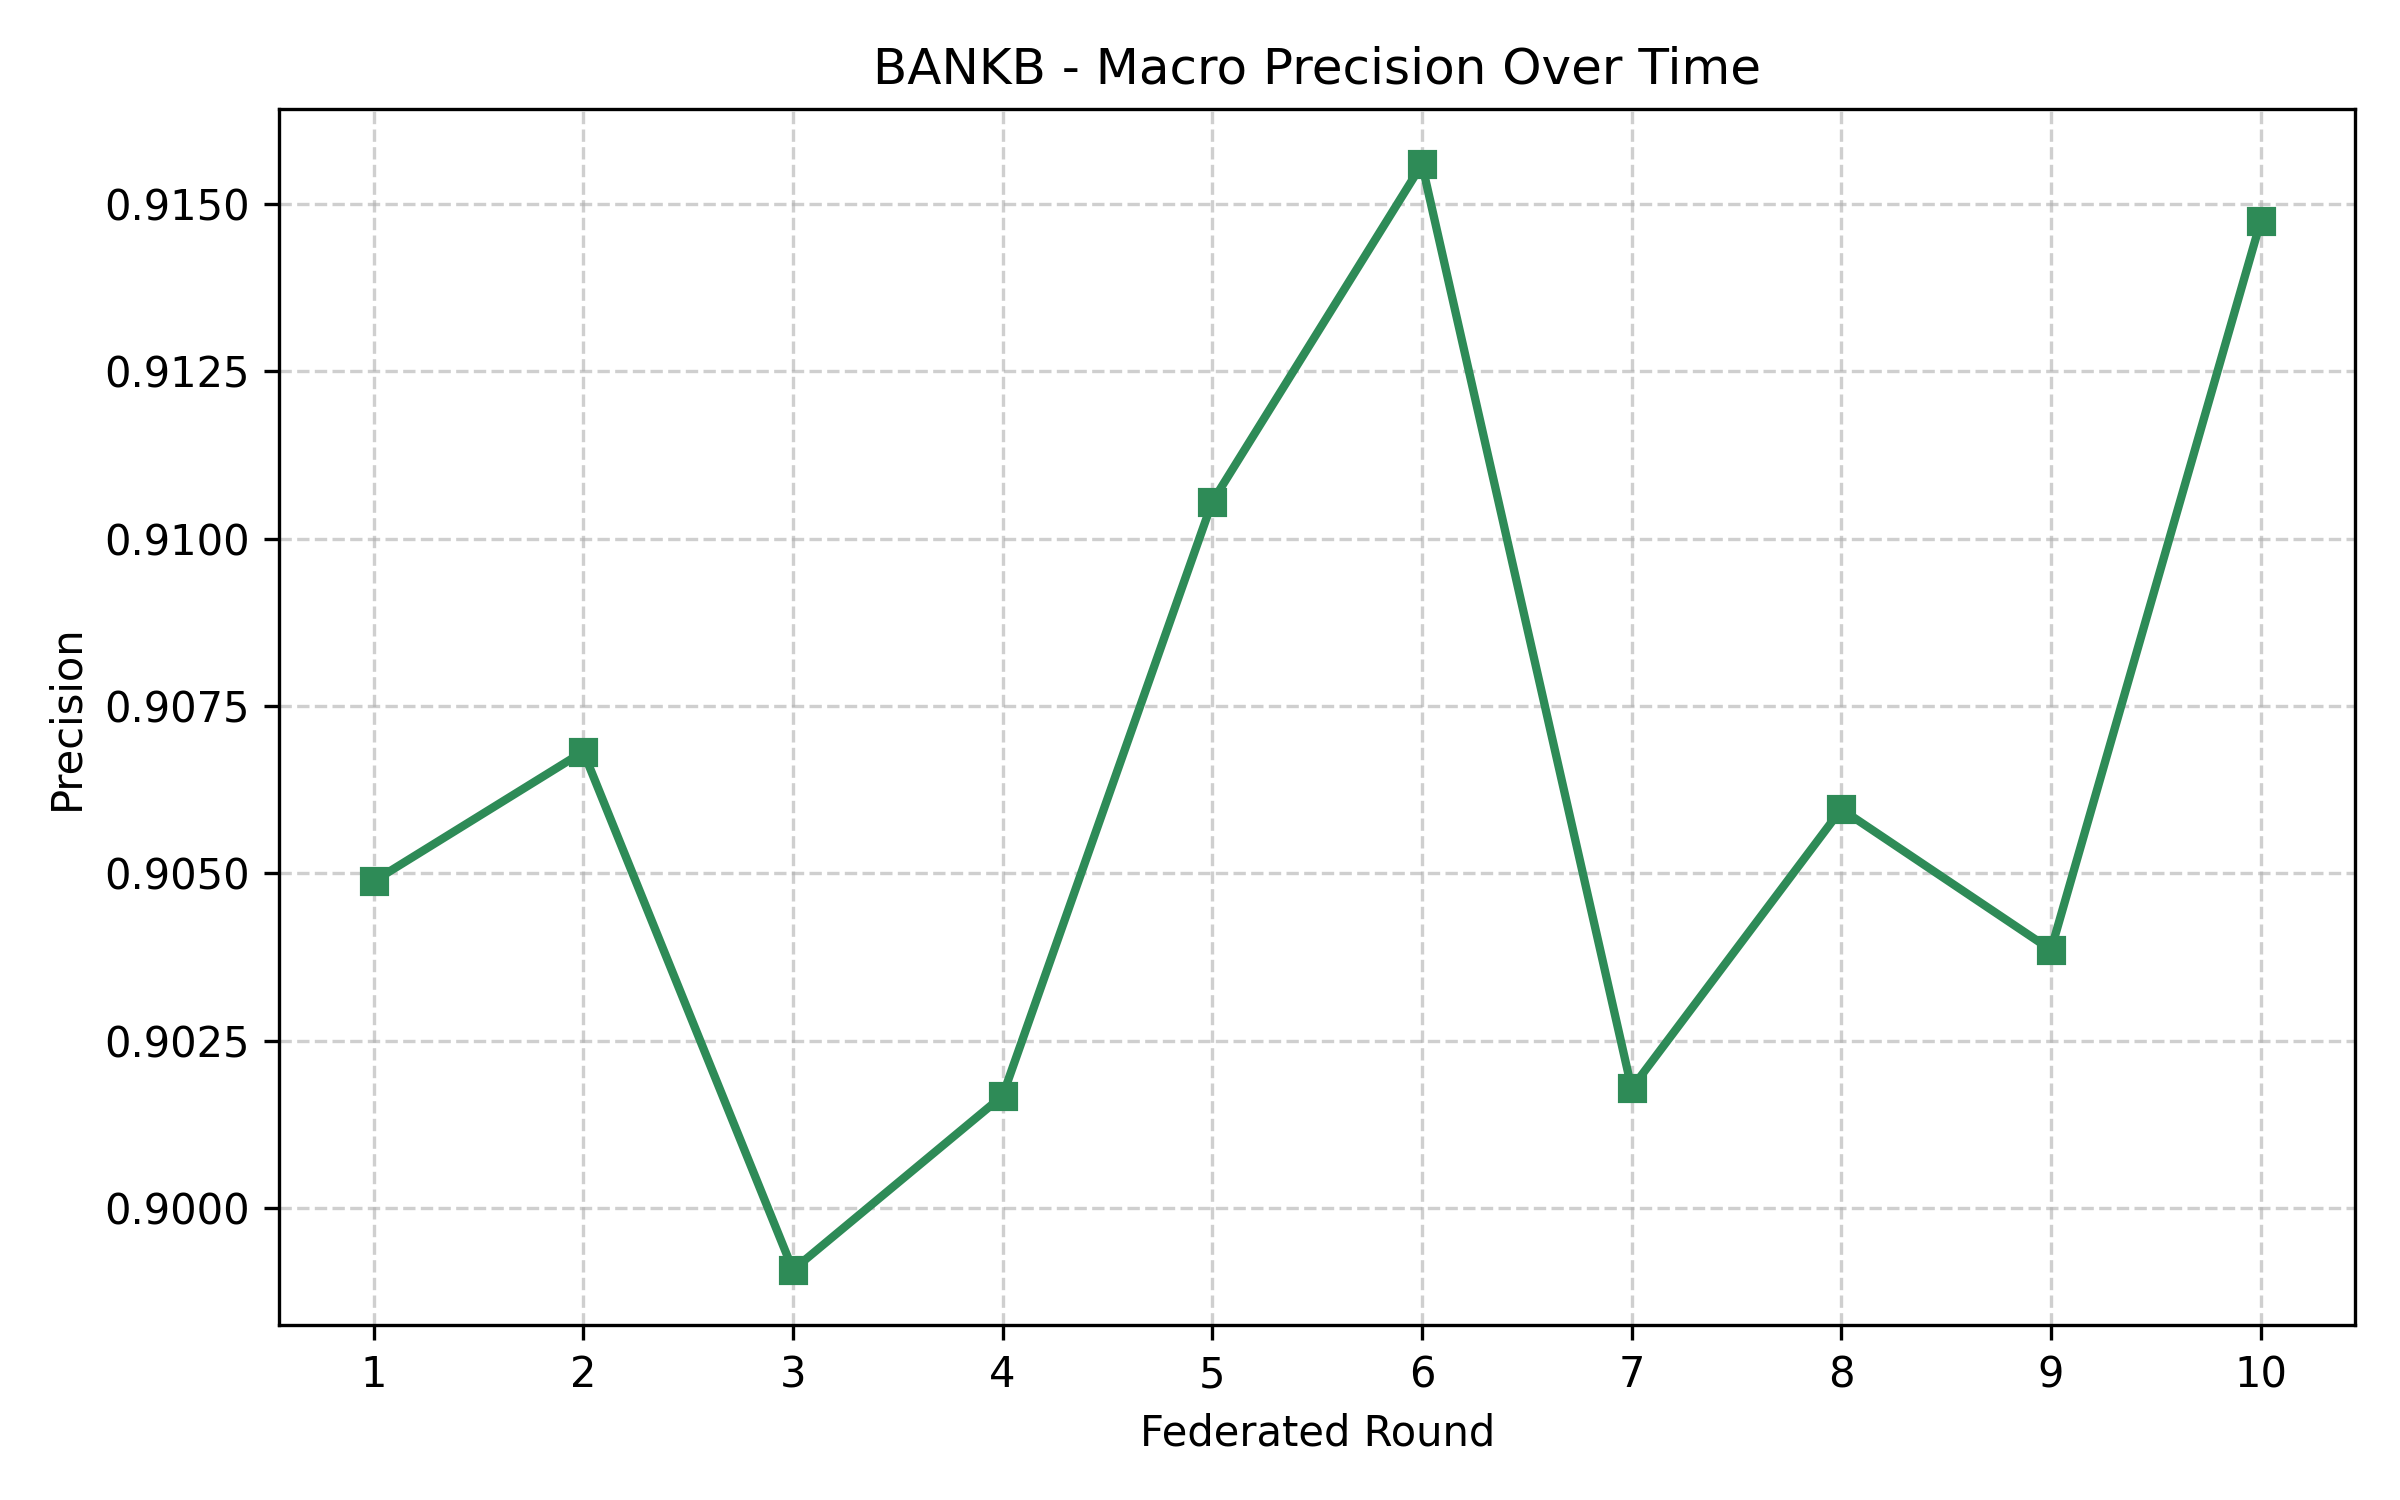
\includegraphics[width=\linewidth]{Figures/bankb_progression_precision.png}
\end{minipage}
\hfill
\begin{minipage}{0.32\textwidth}
\centering
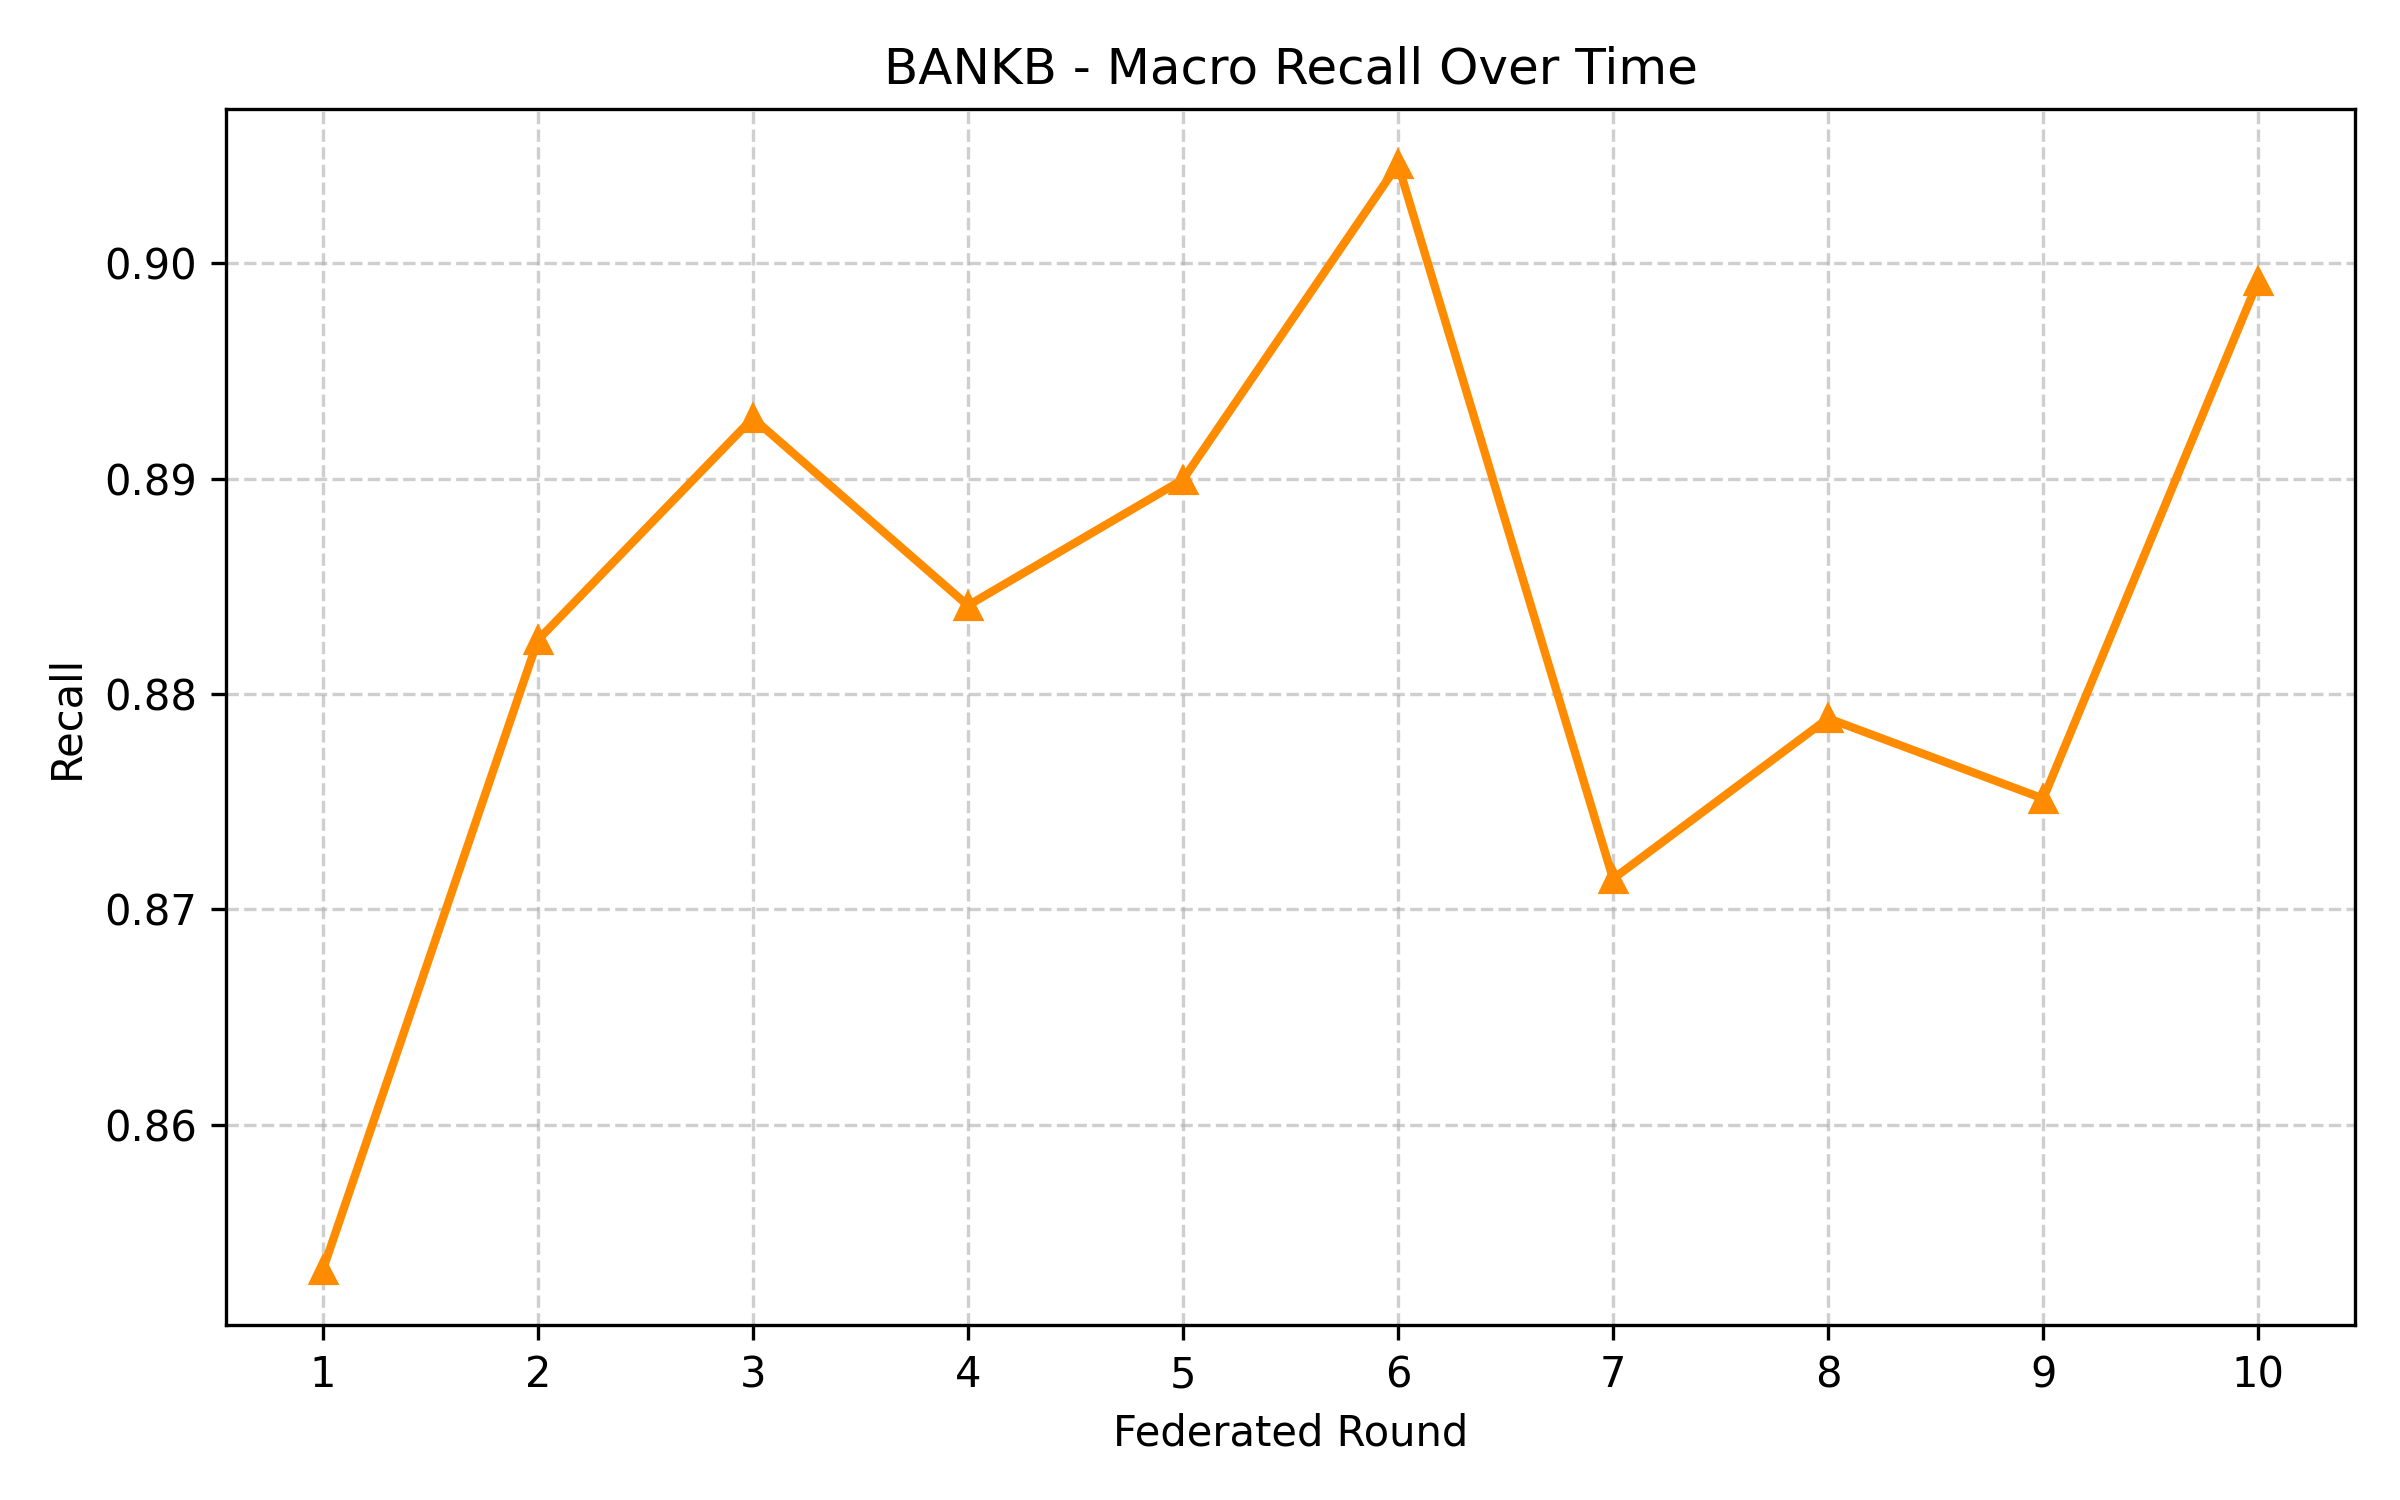
\includegraphics[width=\linewidth]{Figures/bankb_progression_recall.png}
\end{minipage}

\caption{BANKB Federated Accuracy, Precision, and Recall Progression Across Federated Aggregation Rounds}
\label{fig:bankb_progression}
\end{figure}

As shown in Figure~\ref{fig:bankb_progression}, BANKB followed the same stable convergence pattern across the training rounds. Each communication round improved the consistency of the learned parameters and reduced variance in the predictions, which is what we expect when the global model is being updated from multiple institutional clients. The smoother progression confirms that cross-bank parameter sharing and distributed learning were operating correctly.
%--------------------------------------------------------
\subsubsection{BANKC Federated Convergence}
%--------------------------------------------------------

\begin{figure}[H]
\centering

\begin{minipage}{0.32\textwidth}
\centering
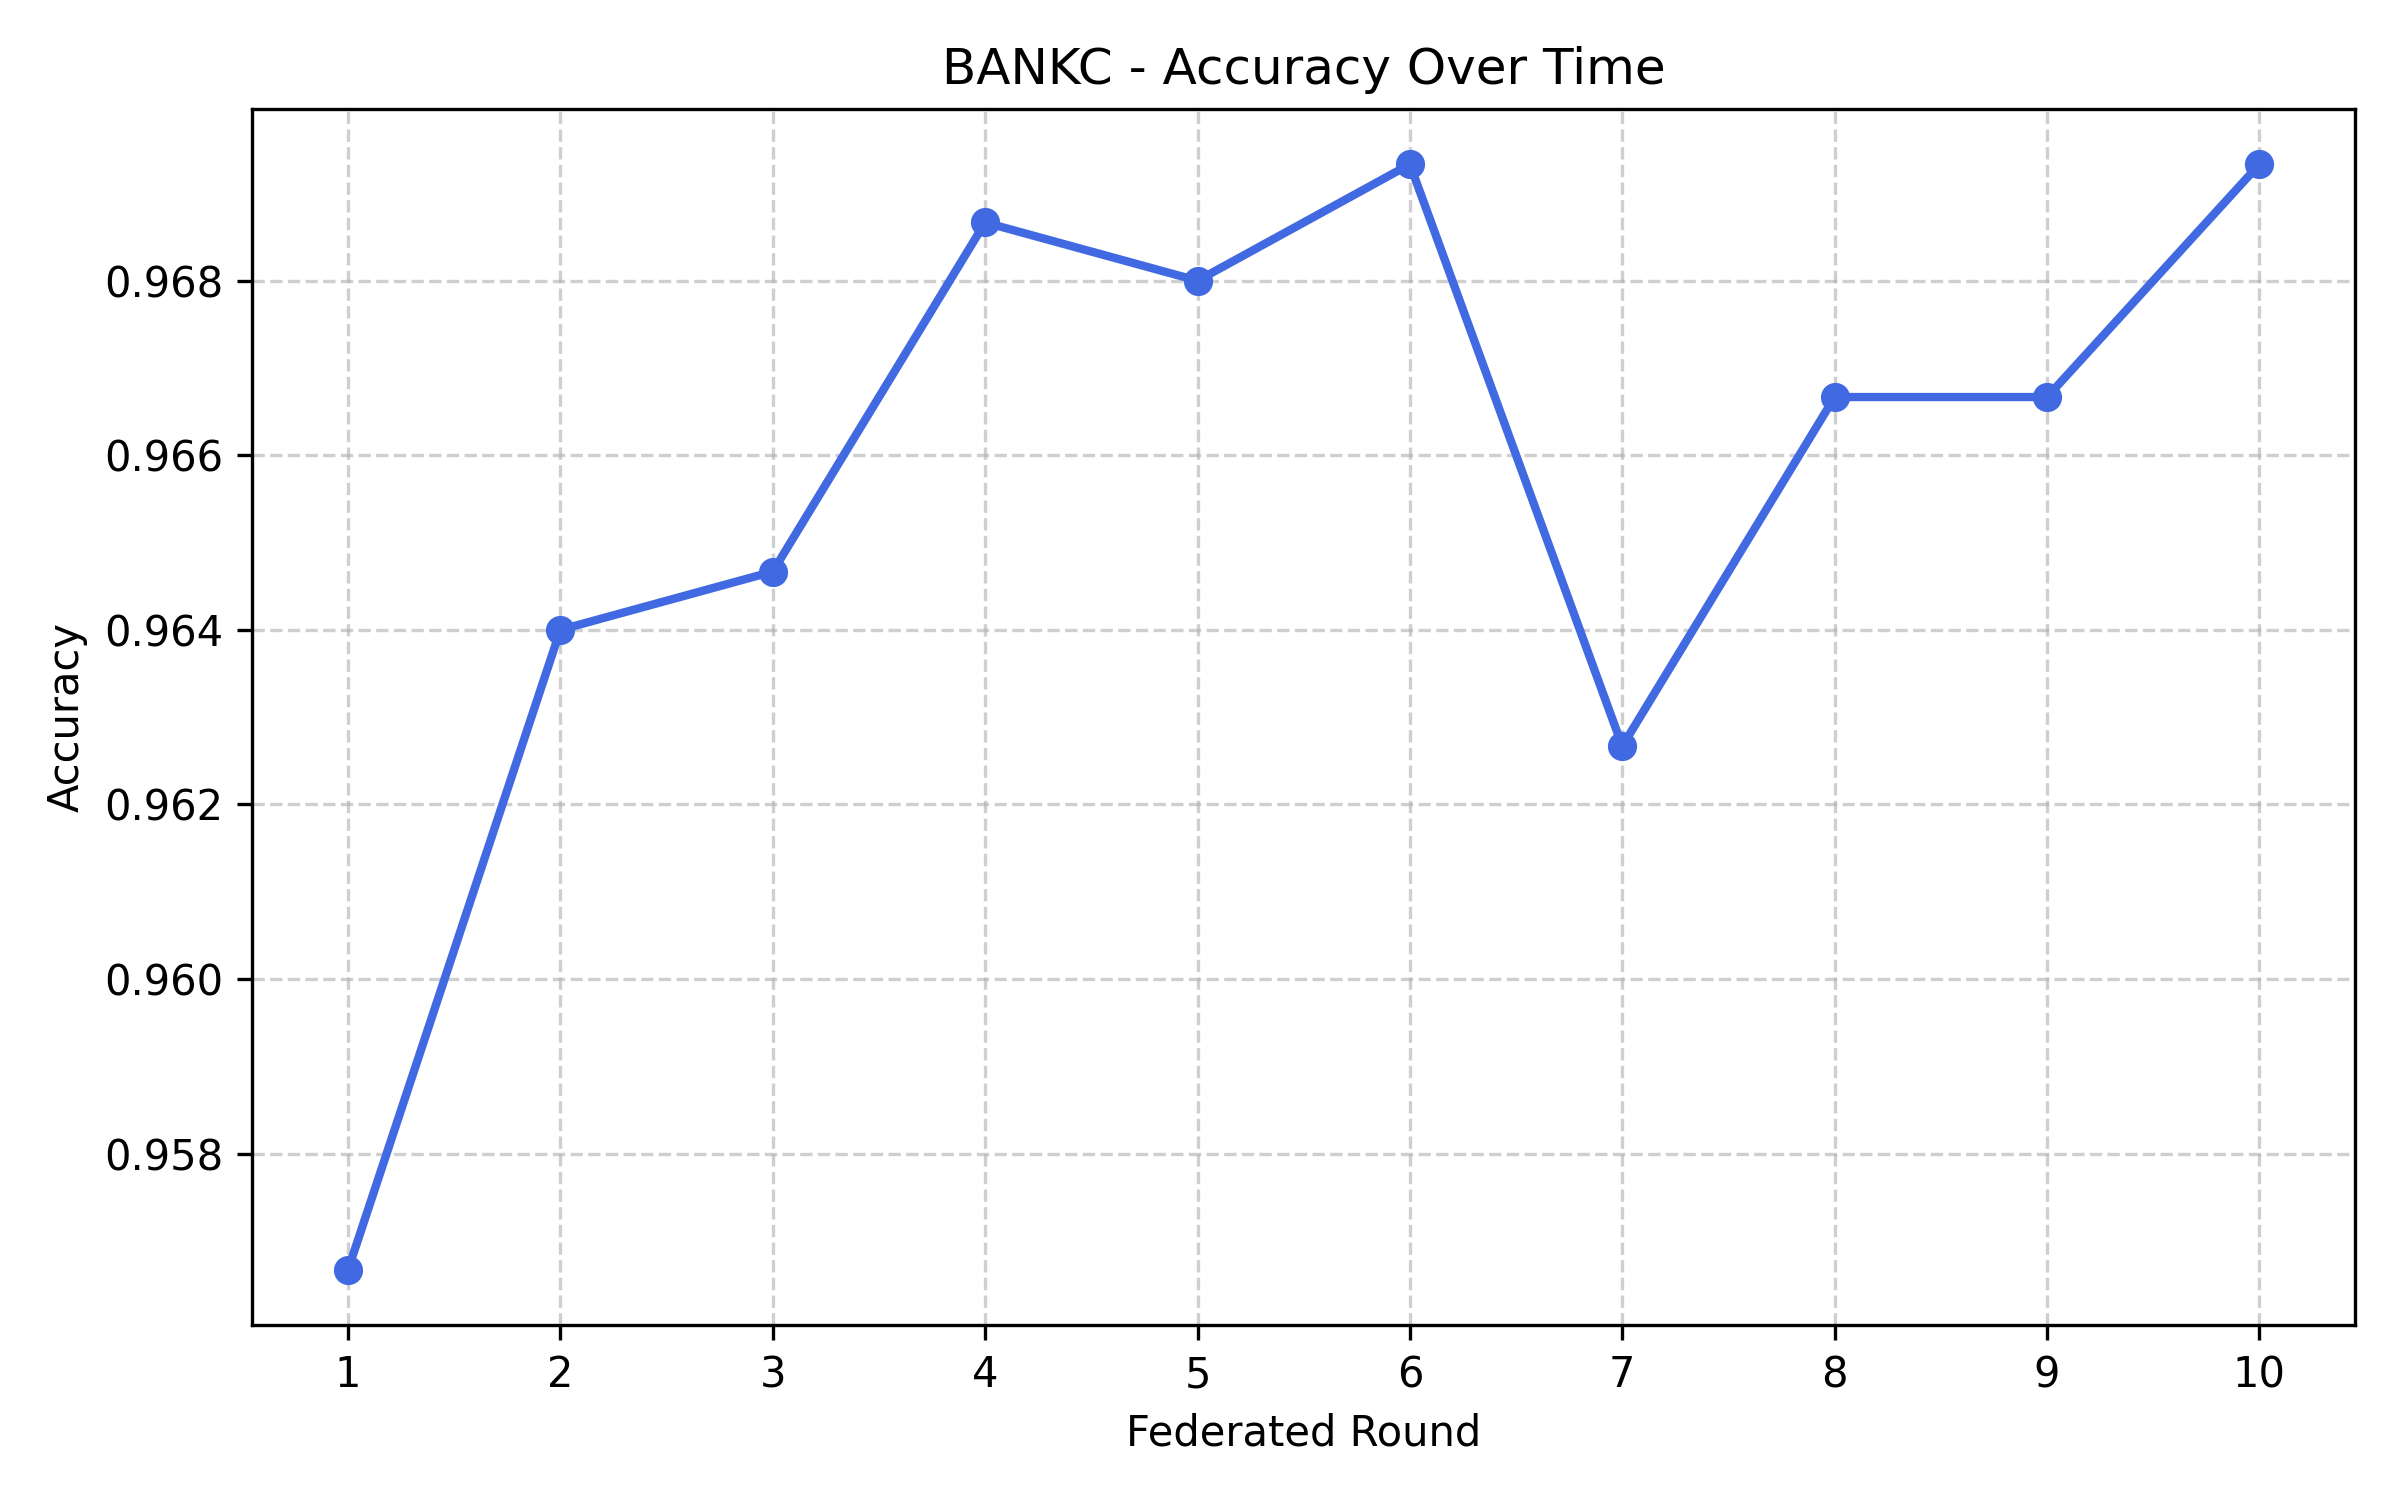
\includegraphics[width=\linewidth]{Figures/bankc_progression_accuracy.png}
\end{minipage}
\hfill
\begin{minipage}{0.32\textwidth}
\centering
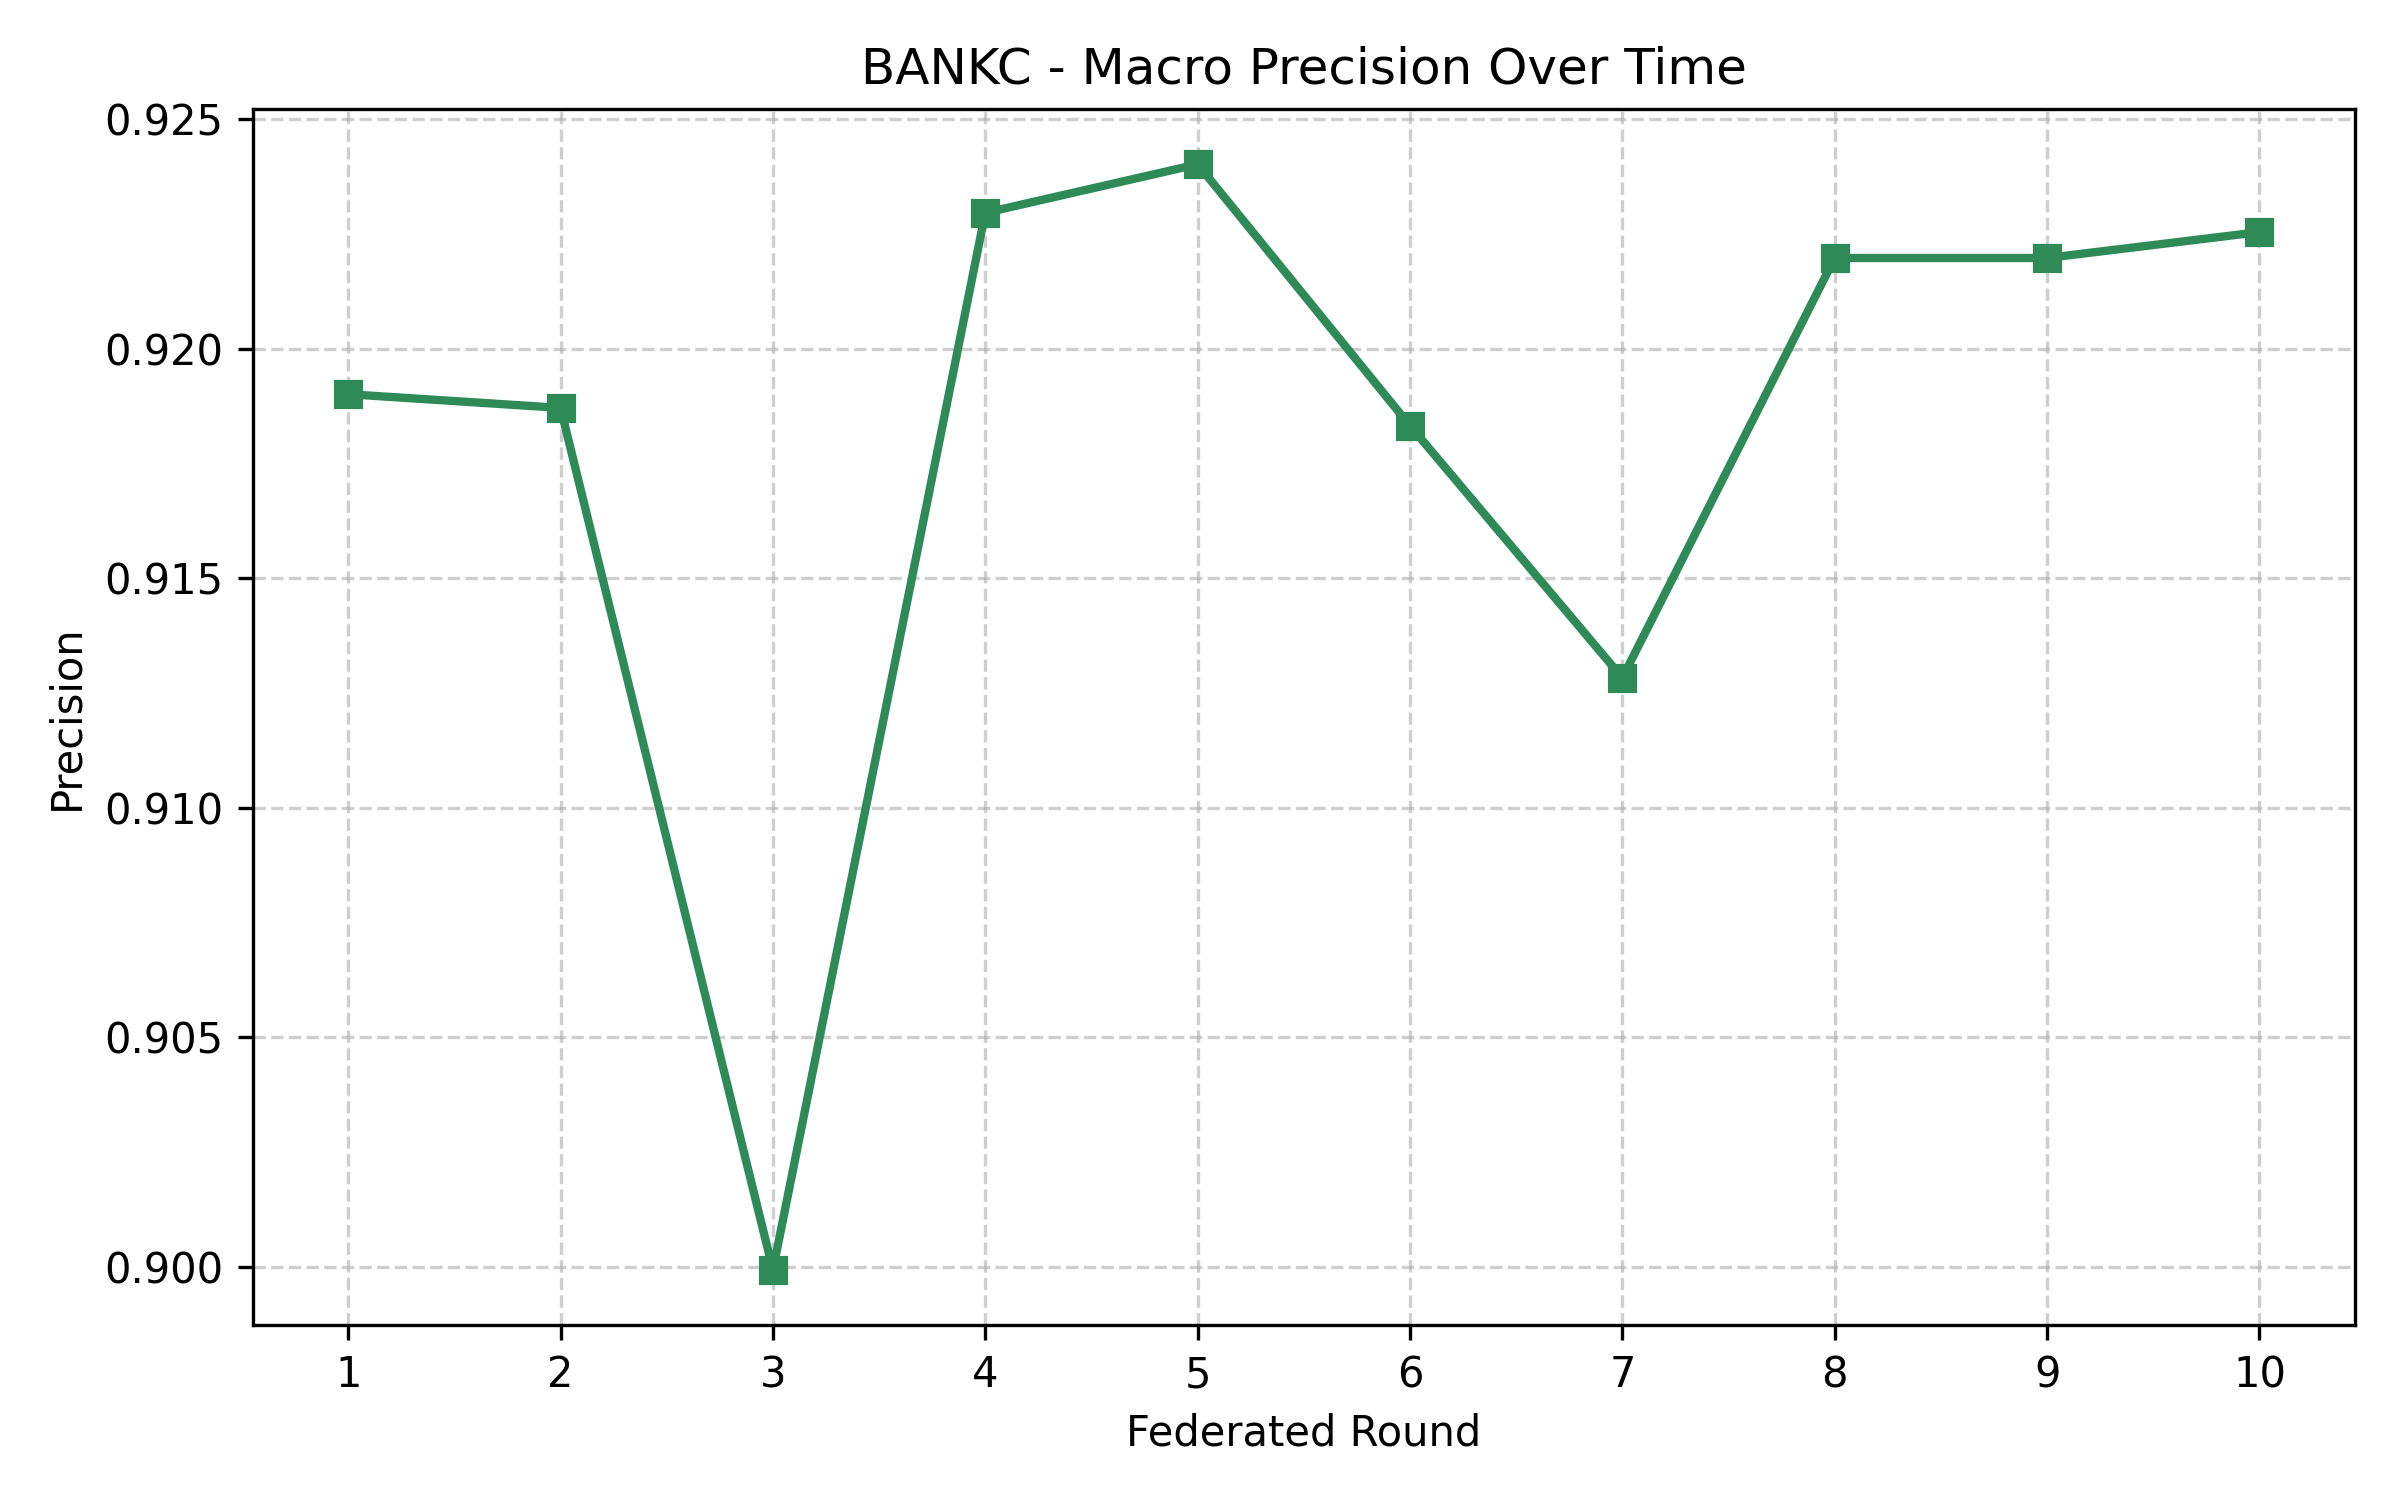
\includegraphics[width=\linewidth]{Figures/bankc_progression_precision.png}
\end{minipage}
\hfill
\begin{minipage}{0.32\textwidth}
\centering
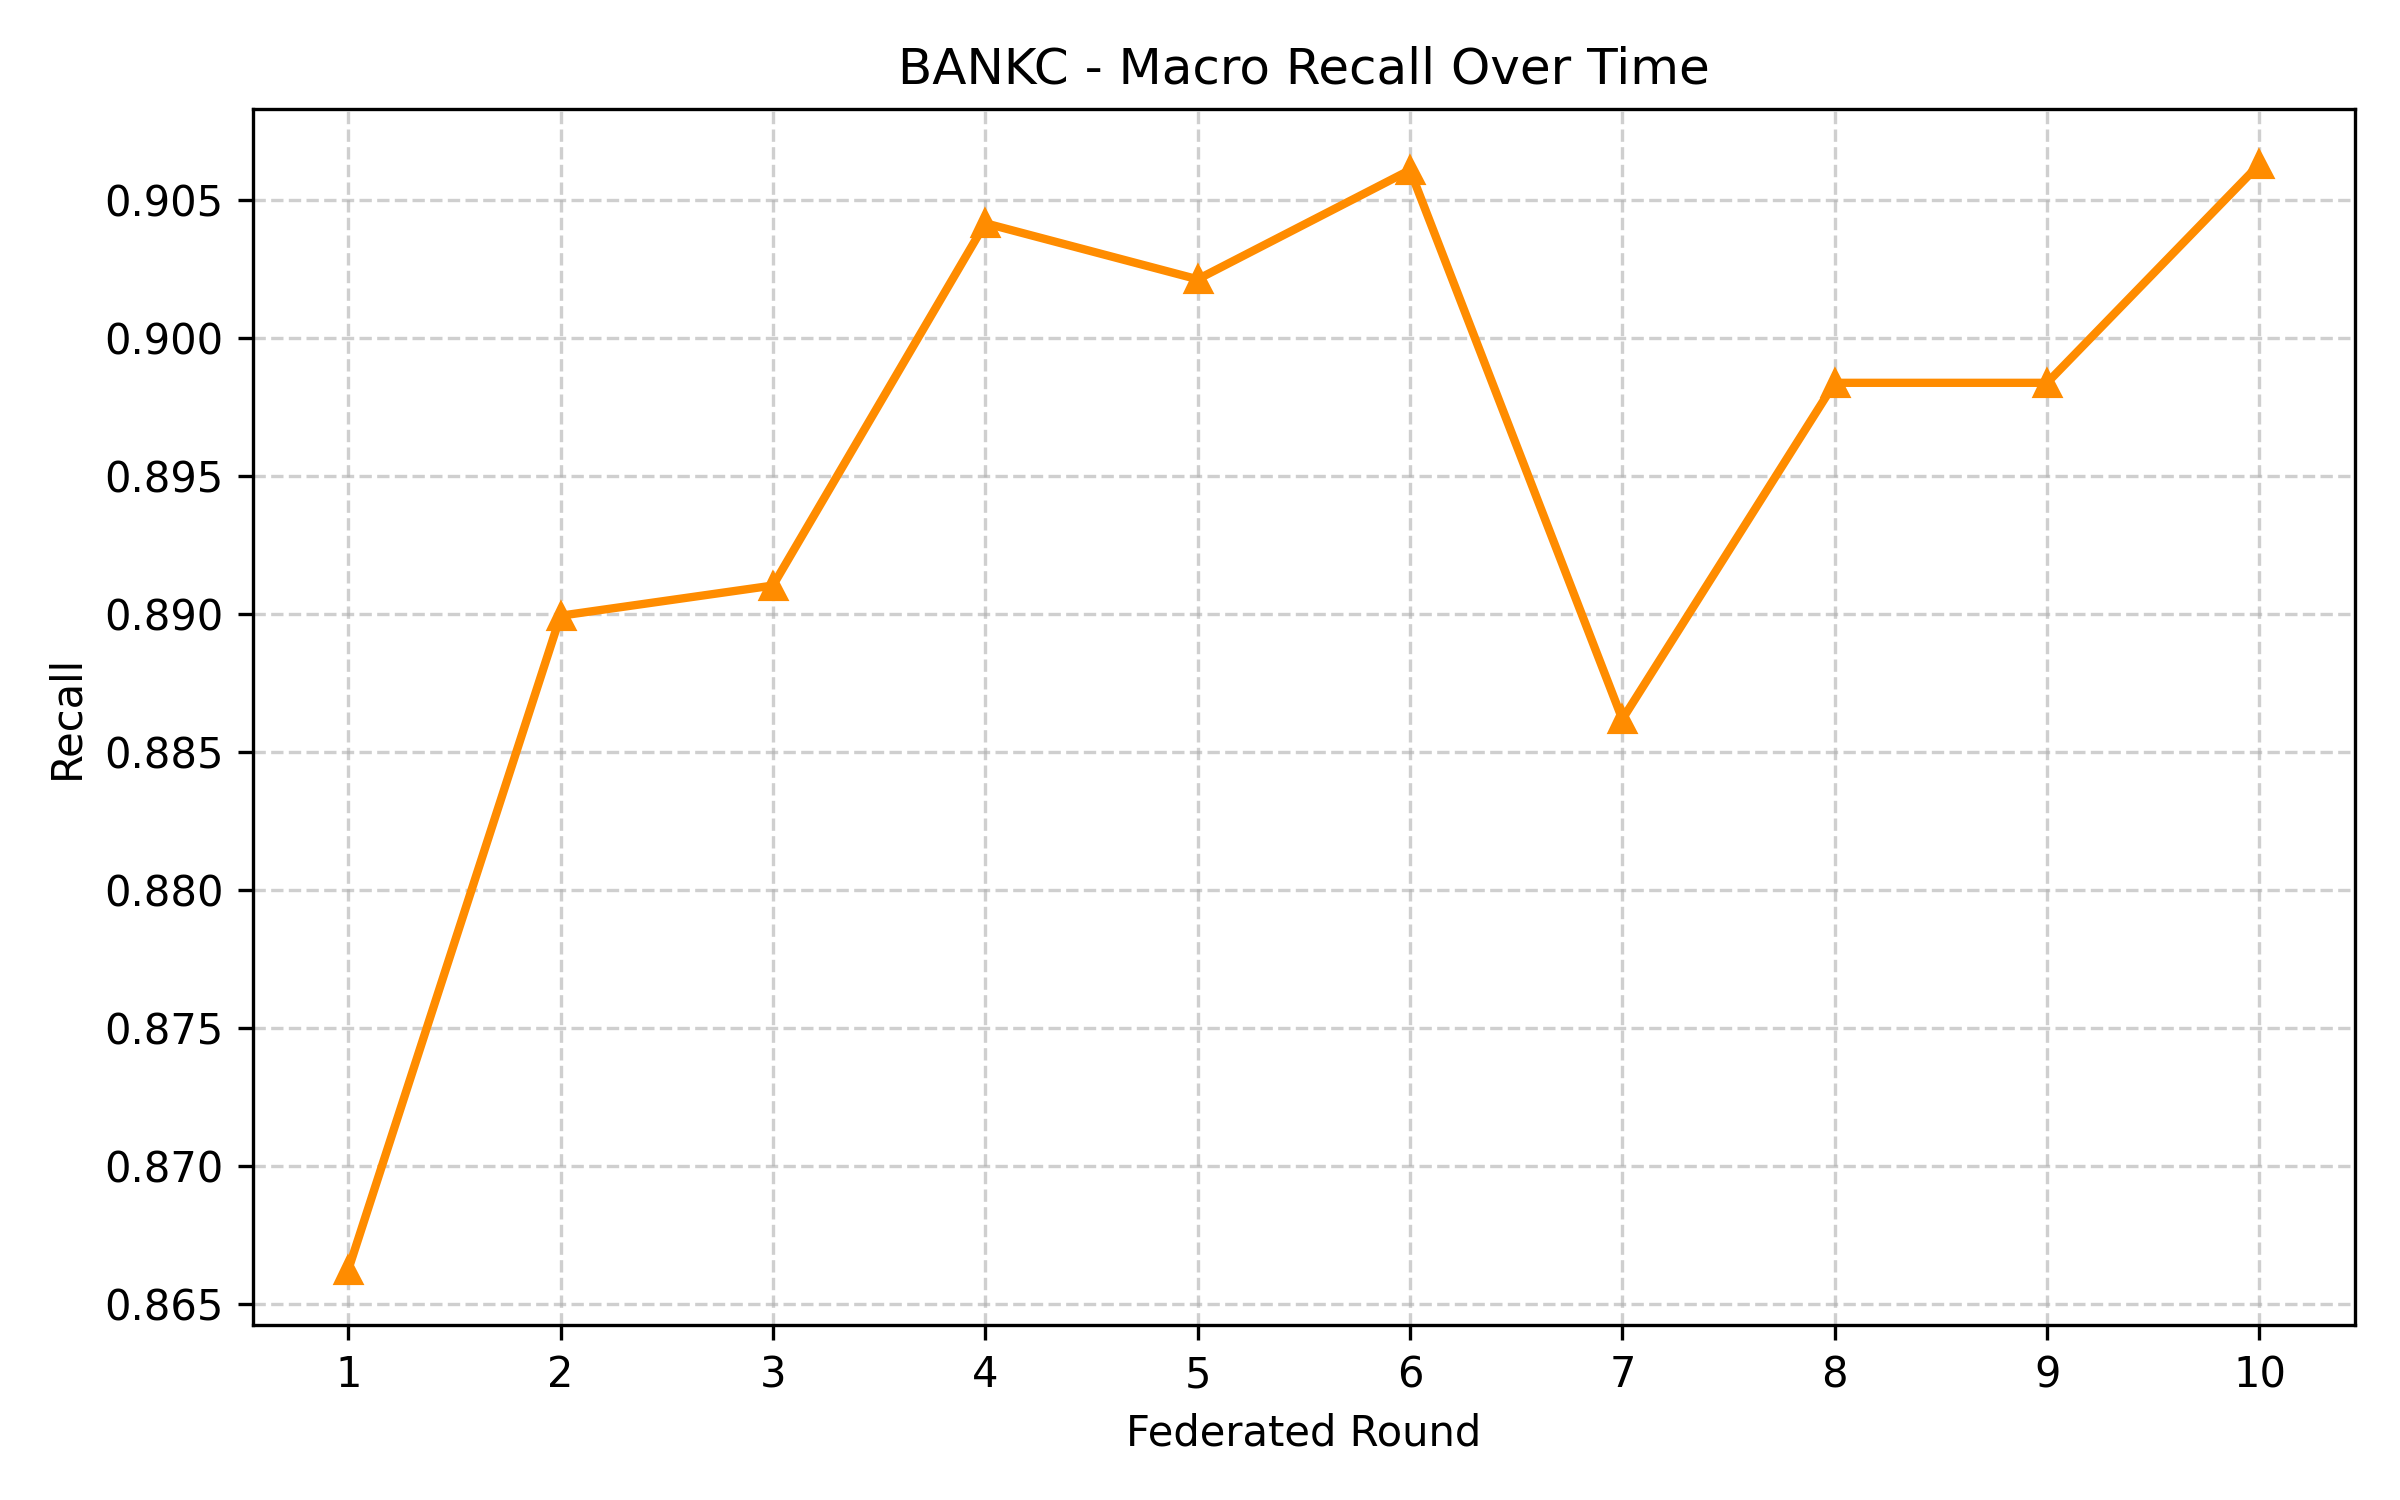
\includegraphics[width=\linewidth]{Figures/bankc_progression_recall.png}
\end{minipage}

\caption{BANKC Federated Accuracy, Precision, and Recall Progression Across Federated Aggregation Rounds}
\label{fig:bankc_progression}
\end{figure}

As shown in Figure~\ref{fig:bankc_progression}, BANKC also converged in a stable and controlled way across the full set of communication rounds. The Accuracy, Precision, and Recall values settled into a consistent range with very little movement in the later stages, which suggests that synchronization was efficient and that the distributed optimization process remained stable. It also indicates that the global model generalized well across different institutional transaction settings.
%========================================================
\subsubsection[Precision--Recall and Confusion Matrix Validation]{\textbf{Precision--Recall and Confusion Matrix Validation}}
%========================================================

Precision--Recall analysis and confusion-matrix evaluation were used to examine how well the framework separated fraud from legitimate activity, especially for the minority classes where the risk of false positives is higher. Since fraudulent transactions represented only a small portion of the full dataset, Precision--Recall gave a clearer picture of model behavior than accuracy alone.

%--------------------------------------------------------
\subsubsection{BANKA Precision--Recall and Confusion Matrix Validation}
%--------------------------------------------------------

\begin{figure}[H]
\centering

\begin{minipage}{0.48\textwidth}
\centering
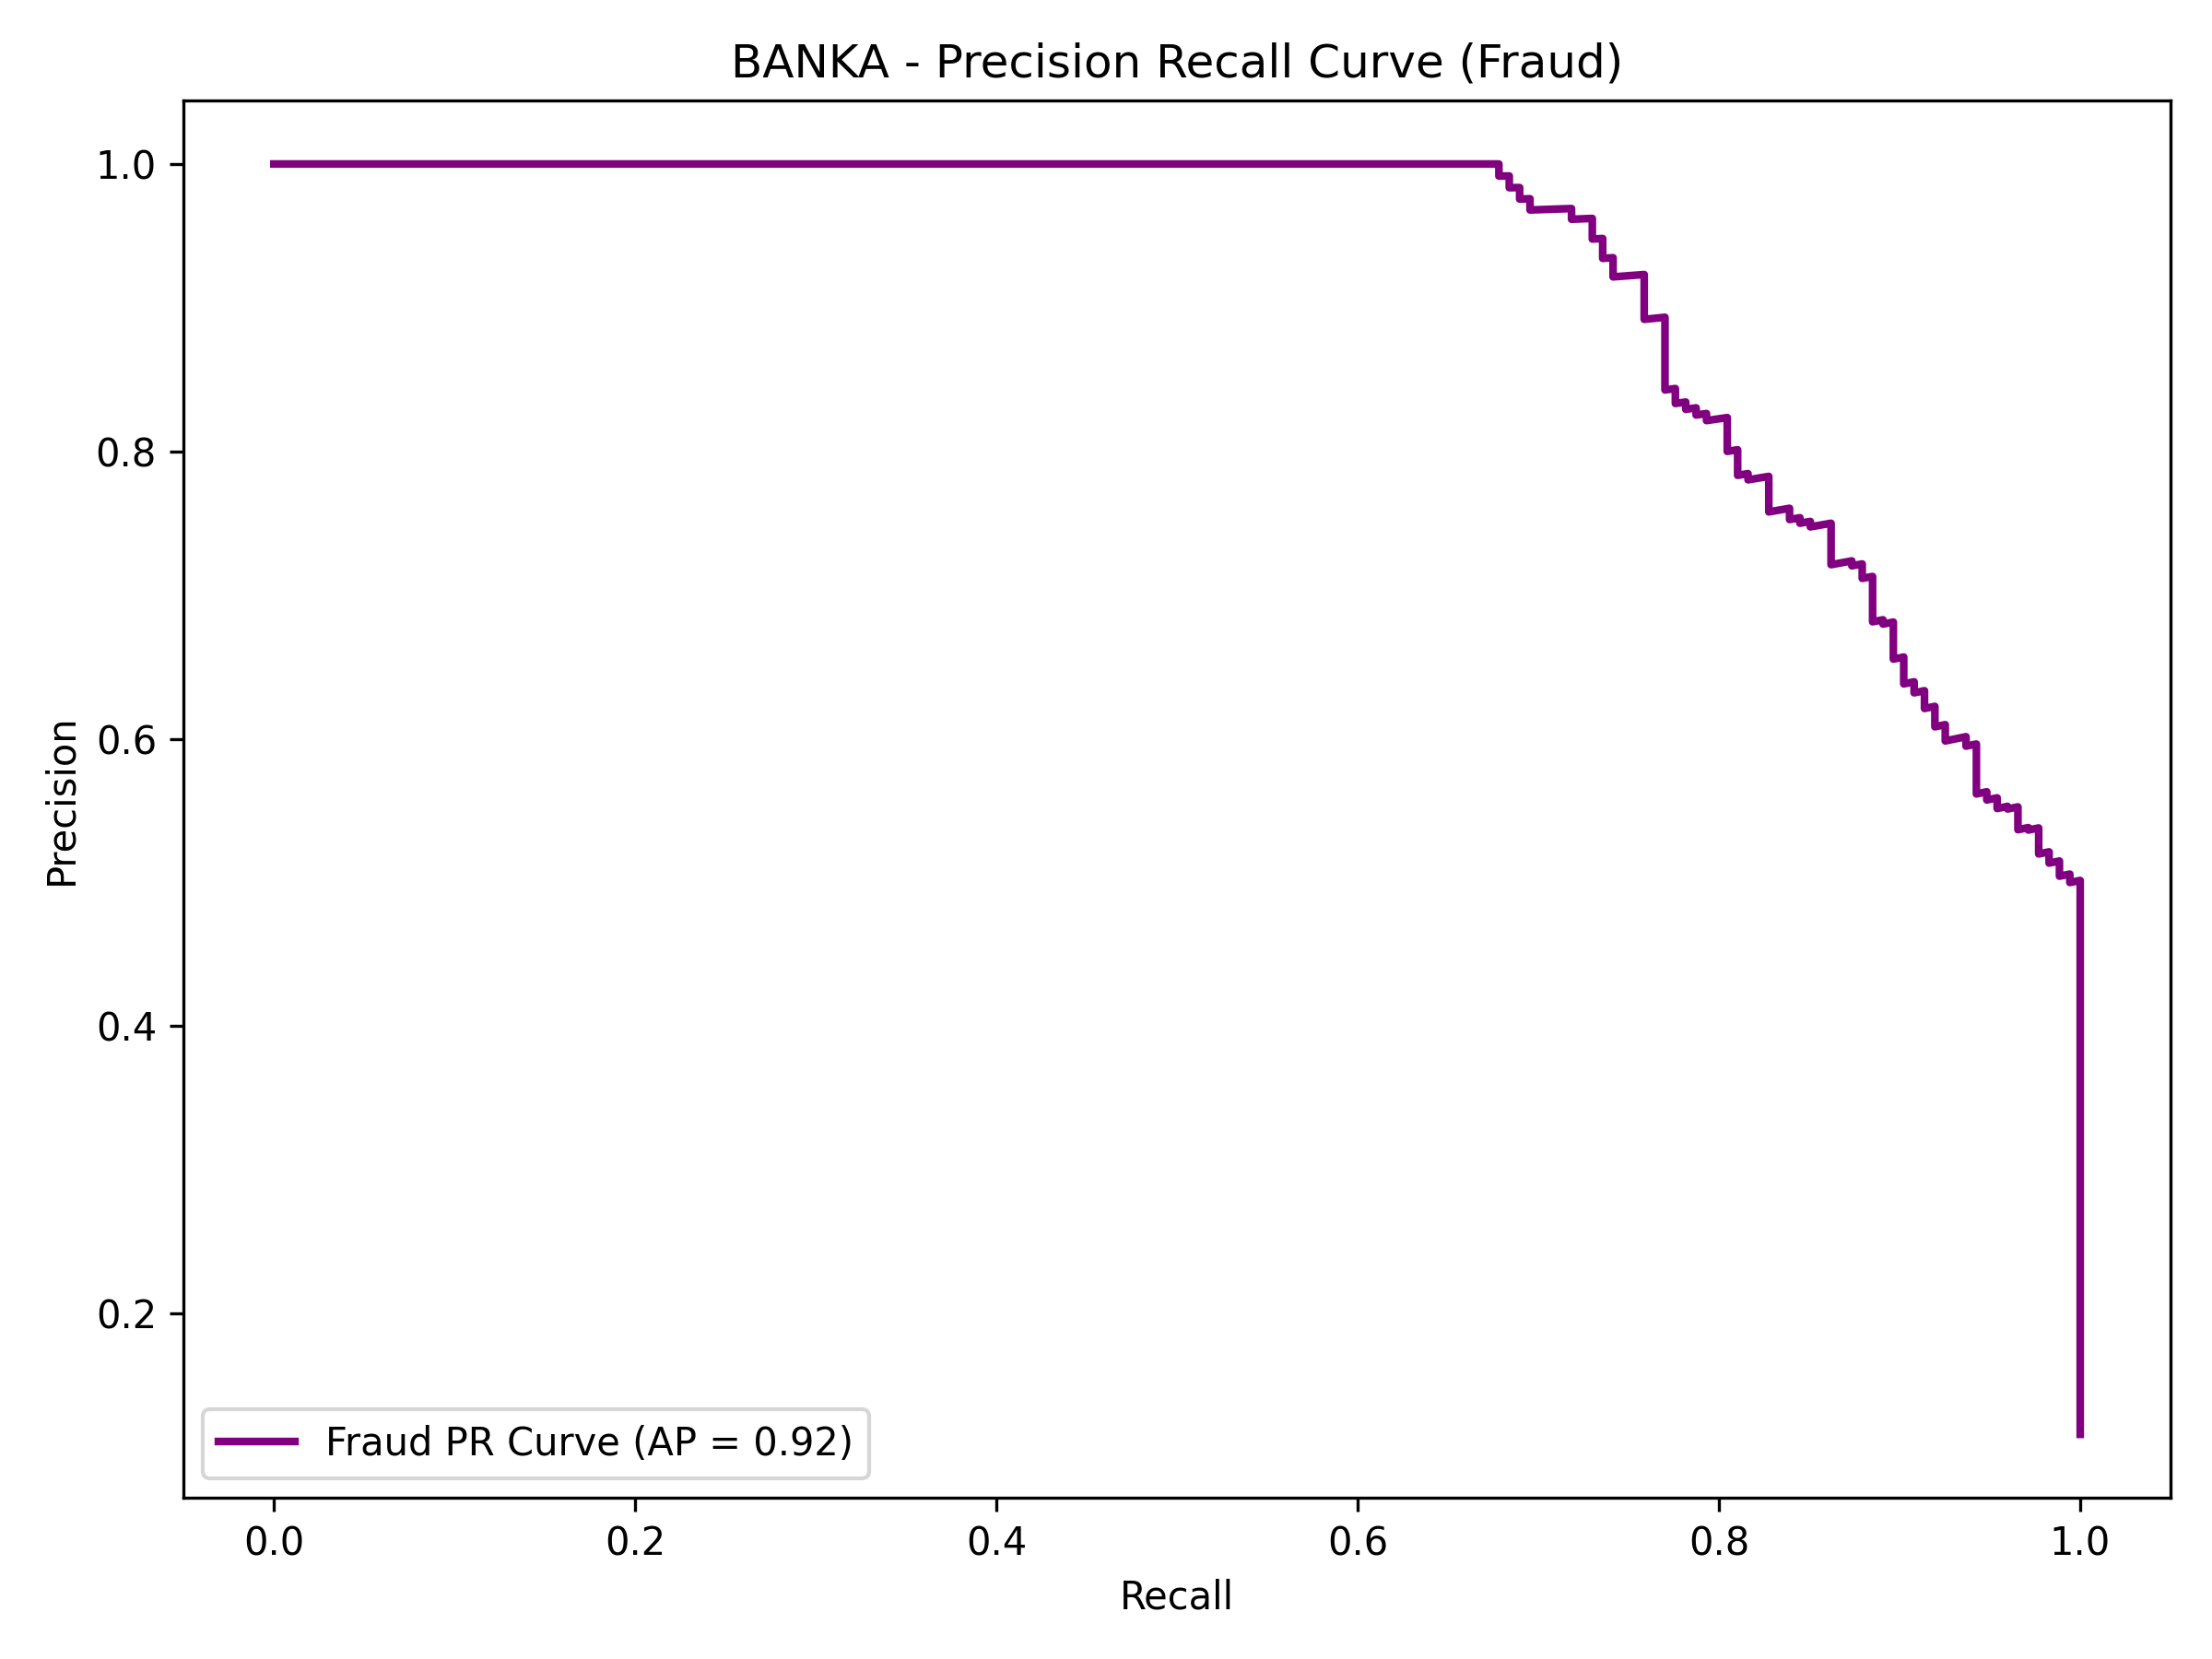
\includegraphics[width=\linewidth]{Figures/banka_pr_curve_deep.png}
\end{minipage}
\hfill
\begin{minipage}{0.48\textwidth}
\centering
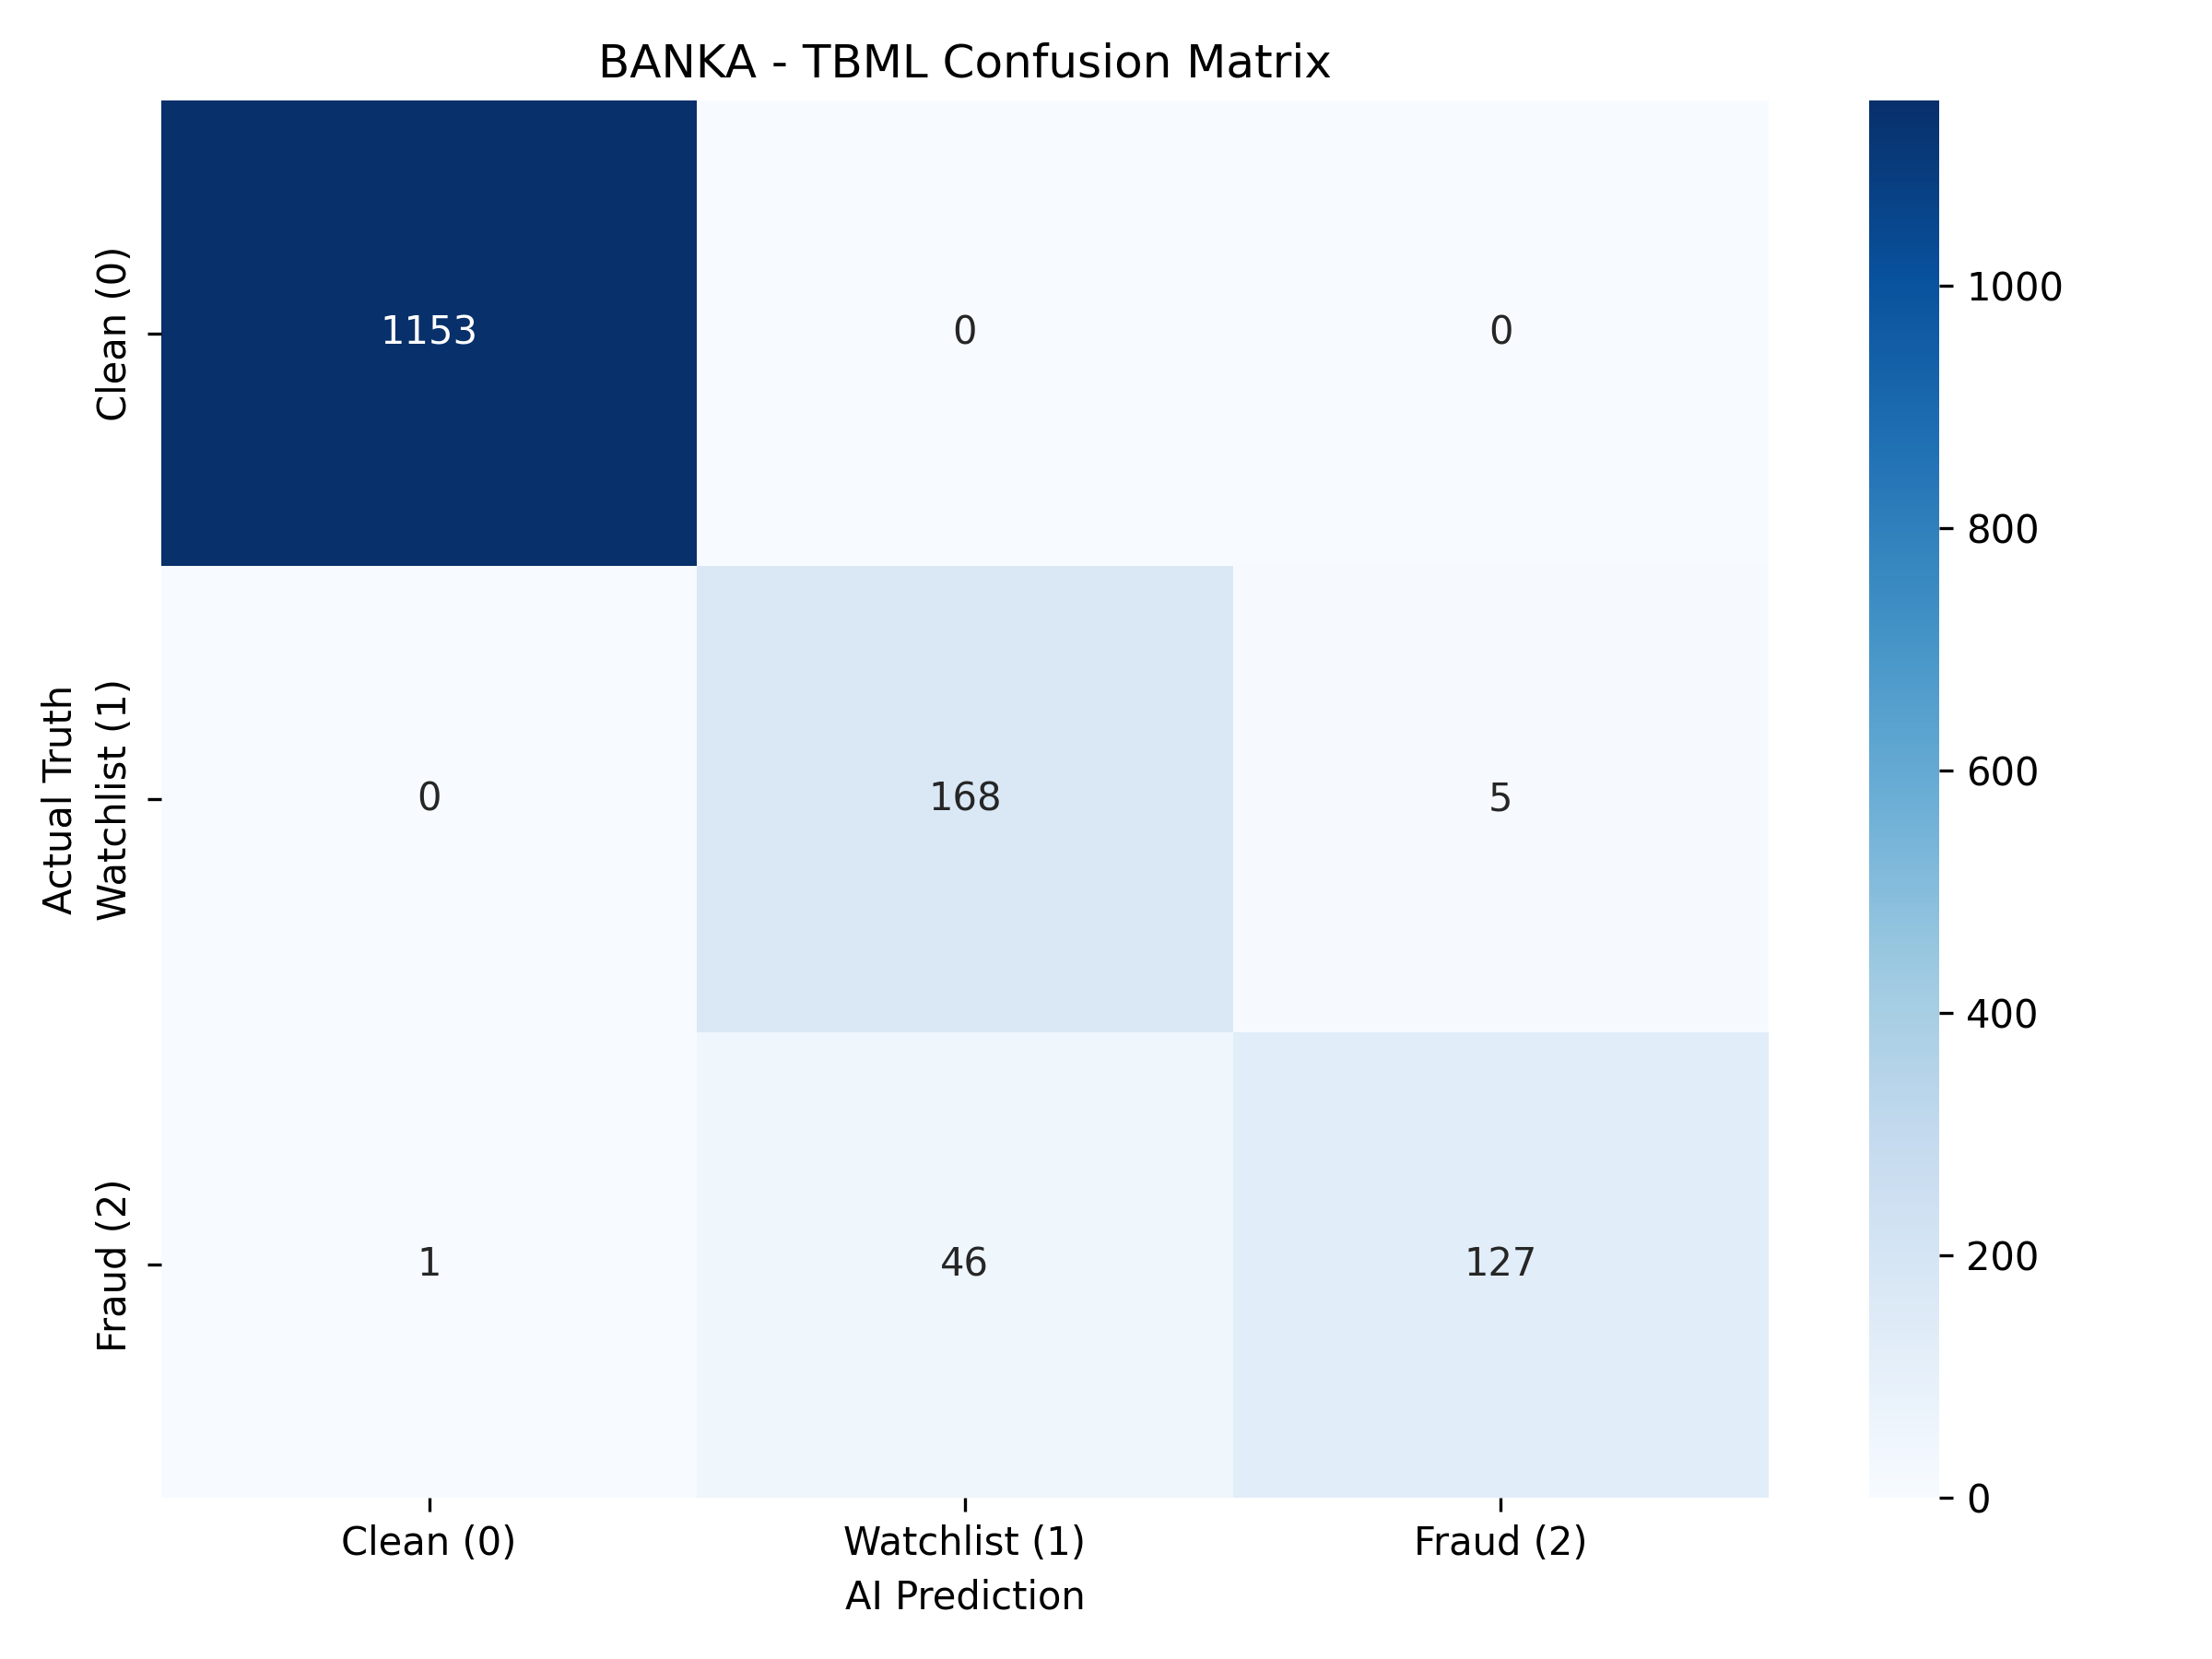
\includegraphics[width=\linewidth]{Figures/banka_confusion_matrix_deep.png}
\end{minipage}

\caption{BANKA Precision--Recall Curve and Confusion Matrix Validation}
\label{fig:banka_validation}
\end{figure}

As shown in Figure~\ref{fig:banka_validation}, BANKA achieved strong Precision--Recall performance, with Average Precision above 0.90. The curve stayed stable even as recall increased, which shows that suspicious activity was still identified reliably under an imbalanced fraud distribution. The confusion matrix also showed near-perfect classification of legitimate transactions, with very little clean-to-fraud confusion. Most overlap appeared between Watchlist and Fraud, which suggests that the model learned the subtle boundary between those two risky states without producing too many false alarms.
%--------------------------------------------------------
\subsubsection{BANKB Precision--Recall and Confusion Matrix Validation}
%--------------------------------------------------------

\begin{figure}[H]
\centering

\begin{minipage}{0.48\textwidth}
\centering
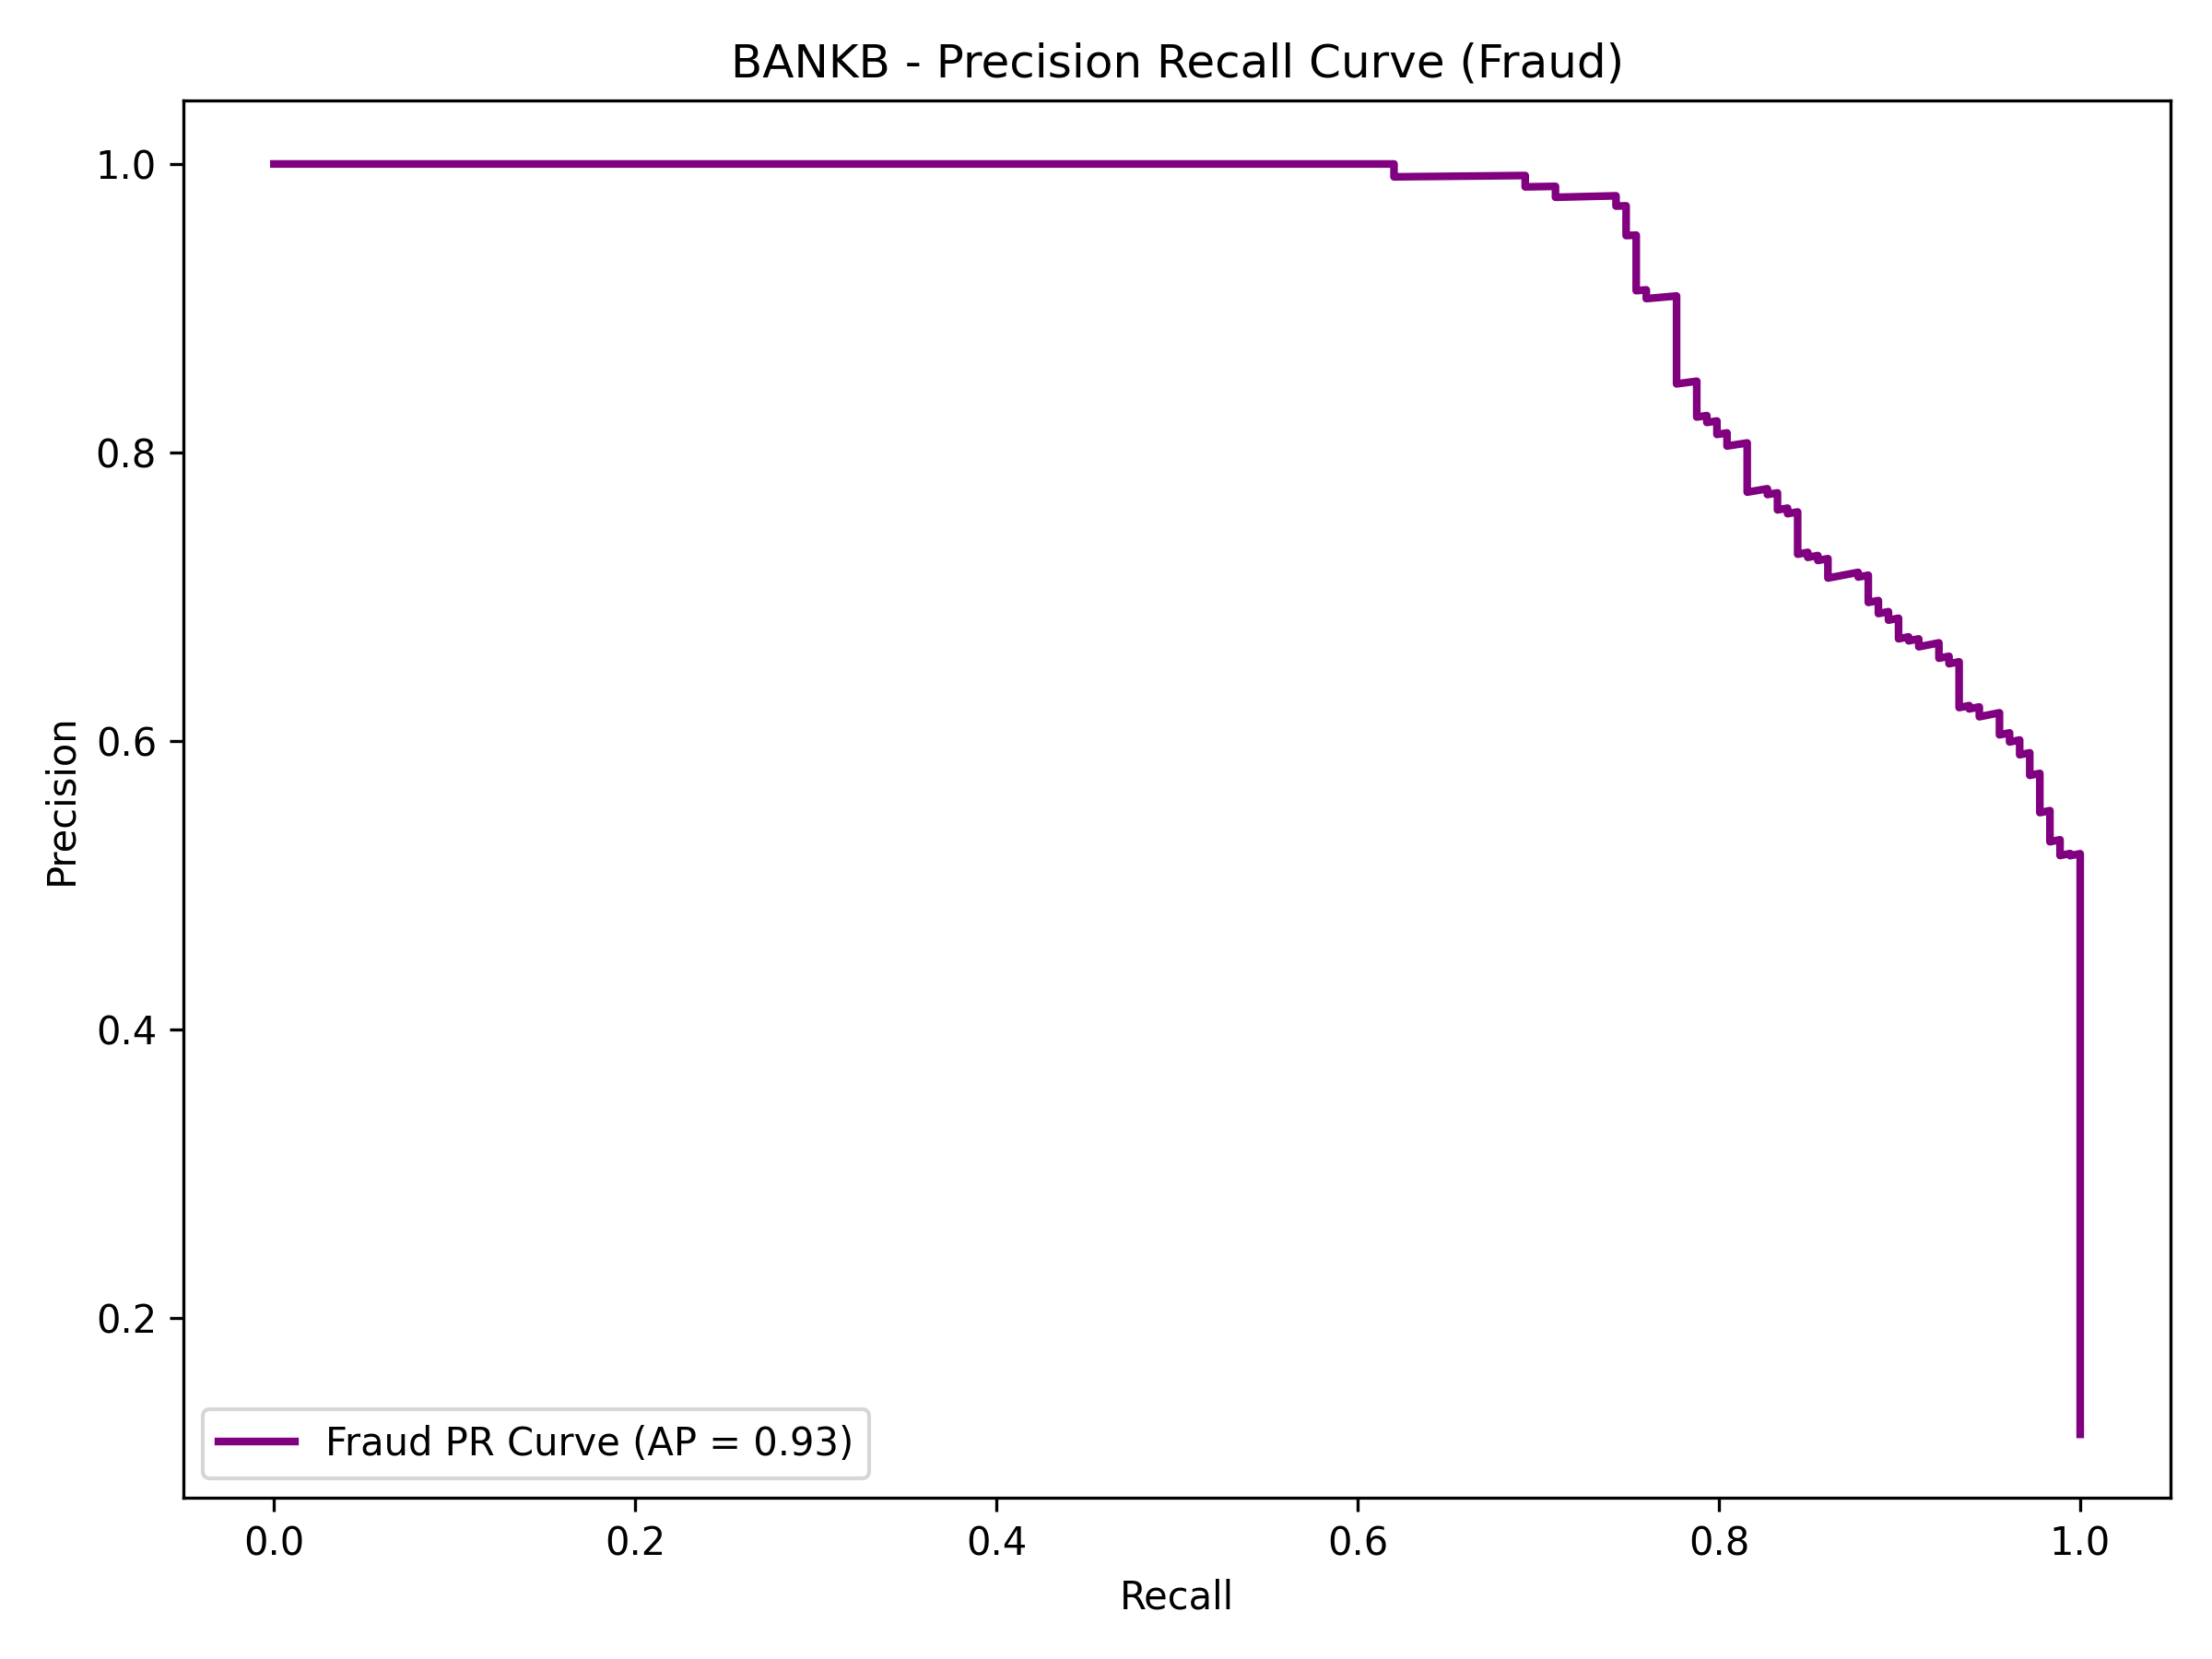
\includegraphics[width=\linewidth]{Figures/bankb_pr_curve_deep.png}
\end{minipage}
\hfill
\begin{minipage}{0.48\textwidth}
\centering
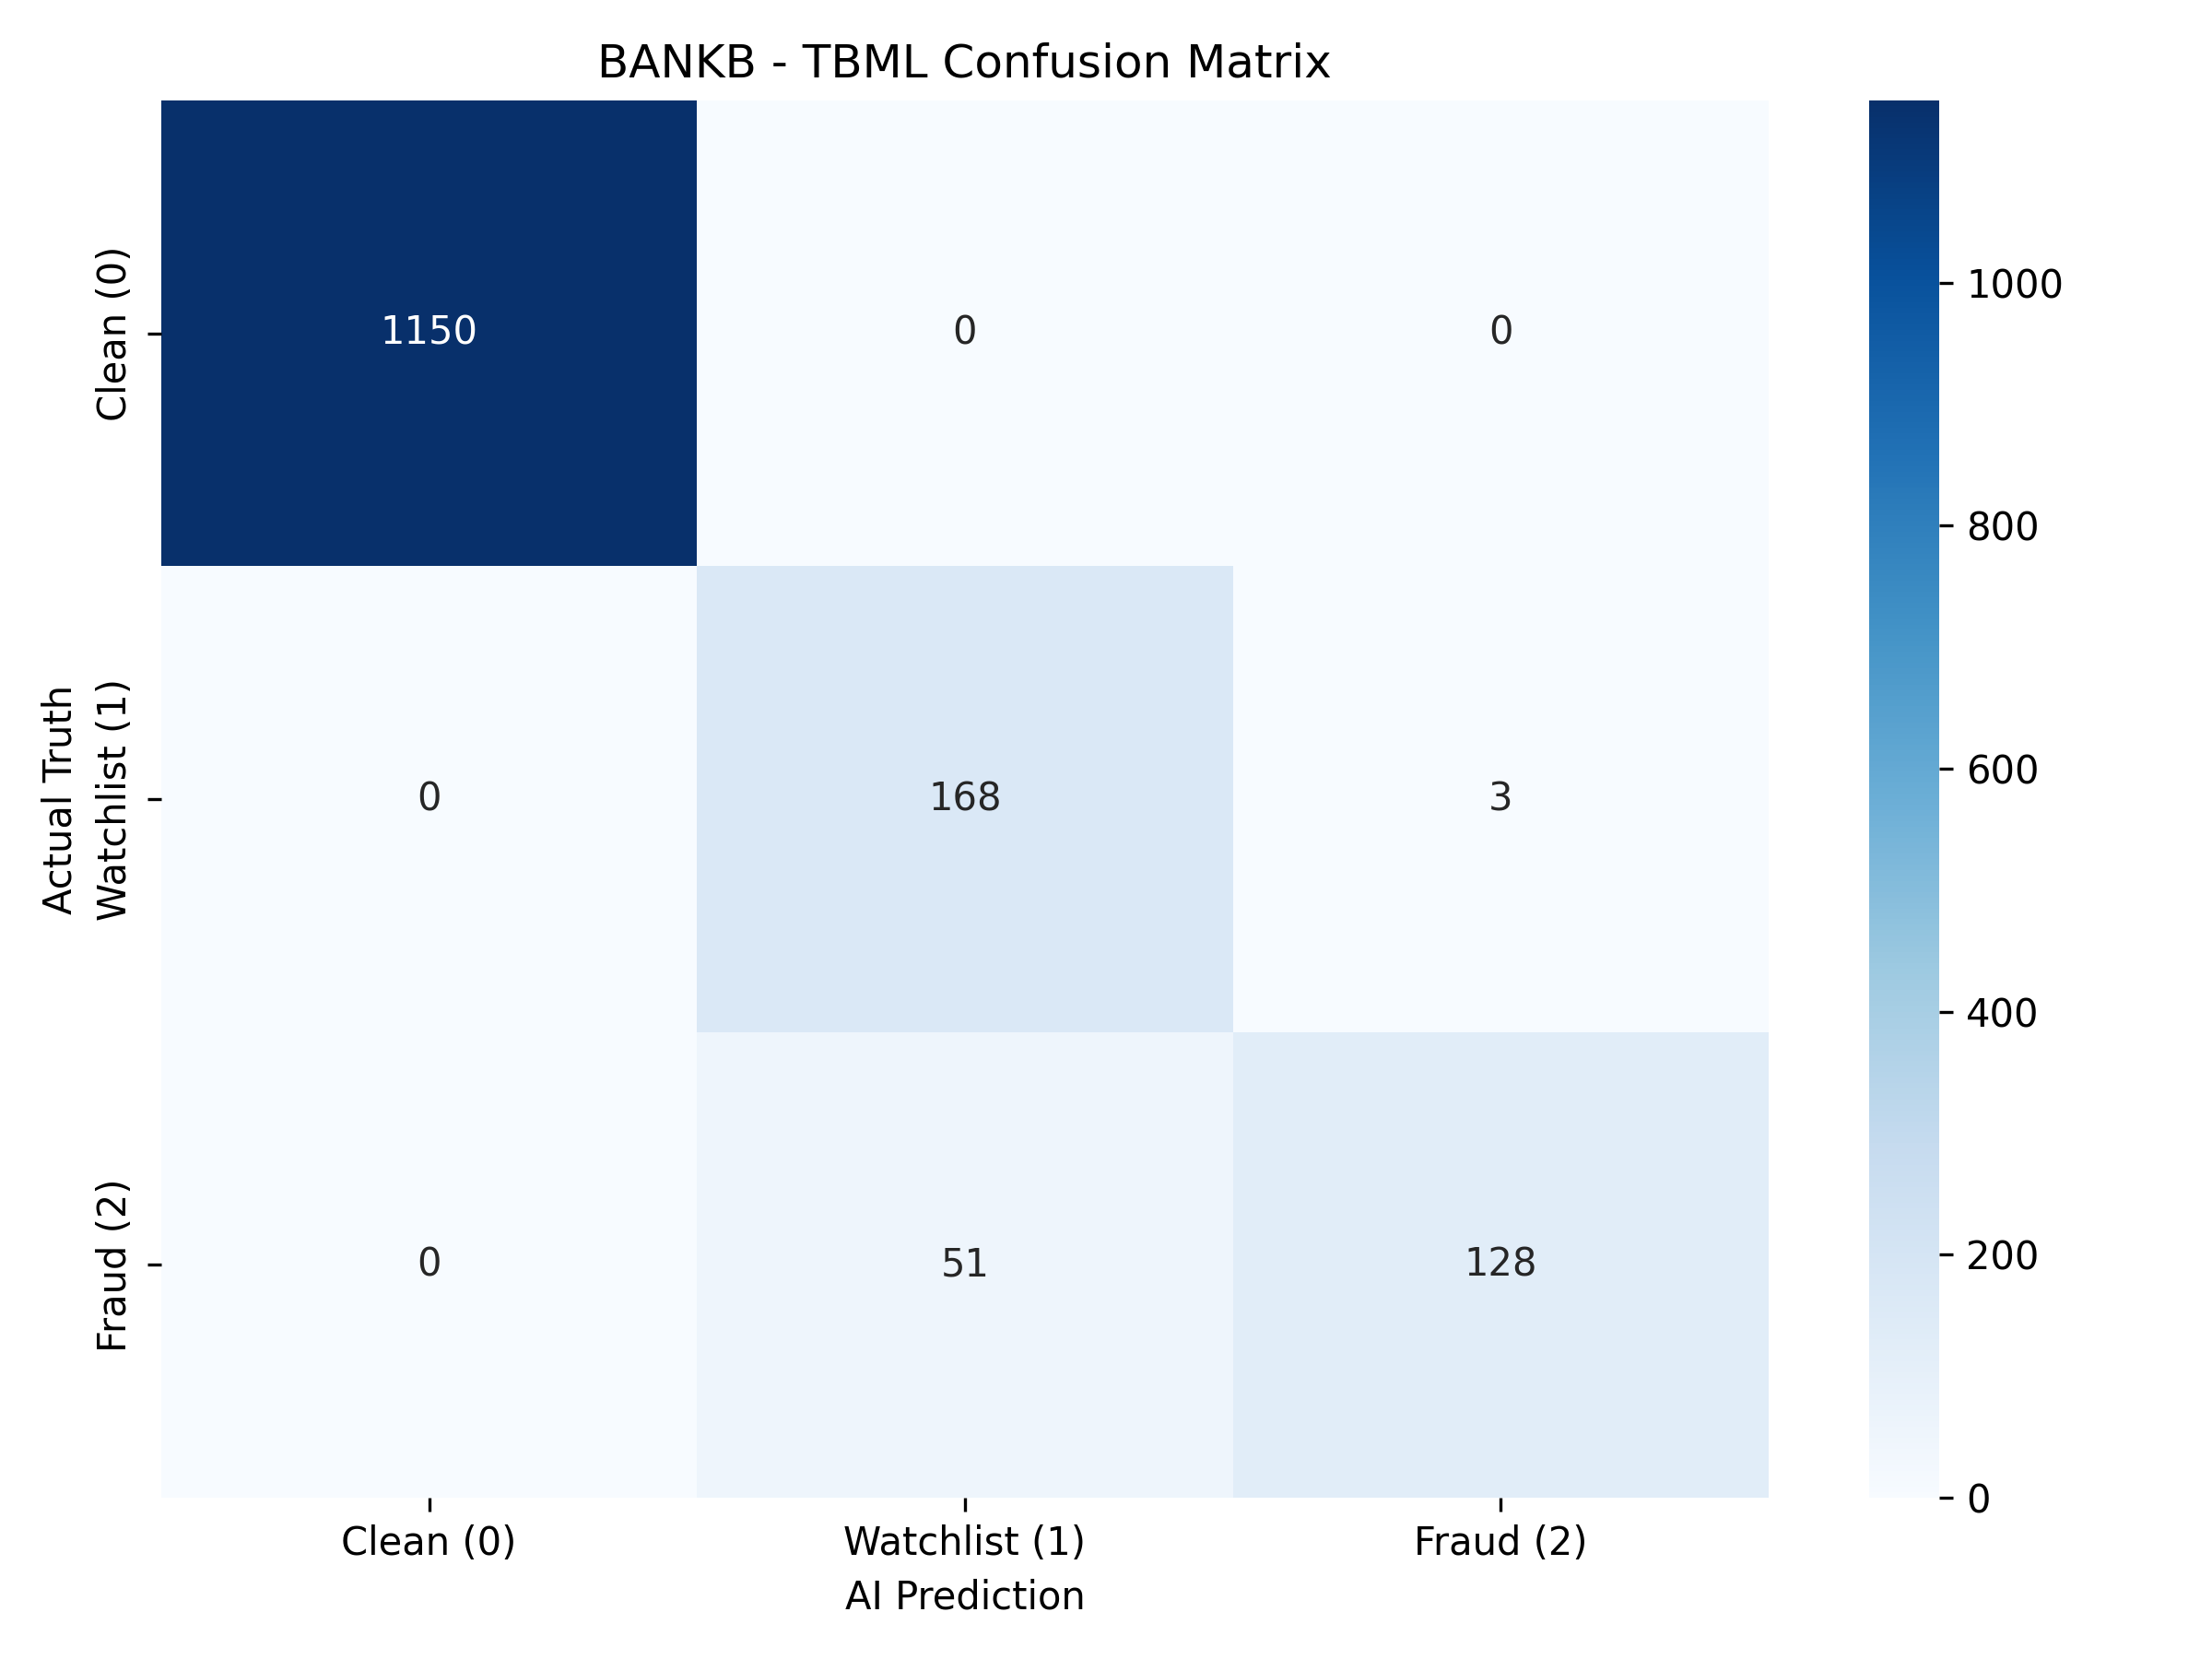
\includegraphics[width=\linewidth]{Figures/bankb_confusion_matrix_deep.png}
\end{minipage}

\caption{BANKB Precision--Recall Curve and Confusion Matrix Validation}
\label{fig:bankb_validation}
\end{figure}

As shown in Figure~\ref{fig:bankb_validation}, BANKB also delivered stable Precision--Recall behavior, again with Average Precision above 0.90. Precision stayed strong as recall increased, which confirms that the model remained sensitive to fraud without losing control over false positives. The confusion matrix showed that legitimate transactions were classified cleanly, and only a small number of Fraud cases were mapped to Watchlist, which indicates solid high-risk discrimination during monitoring.
%--------------------------------------------------------
\subsubsection{BANKC Precision--Recall and Confusion Matrix Validation}
%--------------------------------------------------------

\begin{figure}[H]
\centering

\begin{minipage}{0.48\textwidth}
\centering
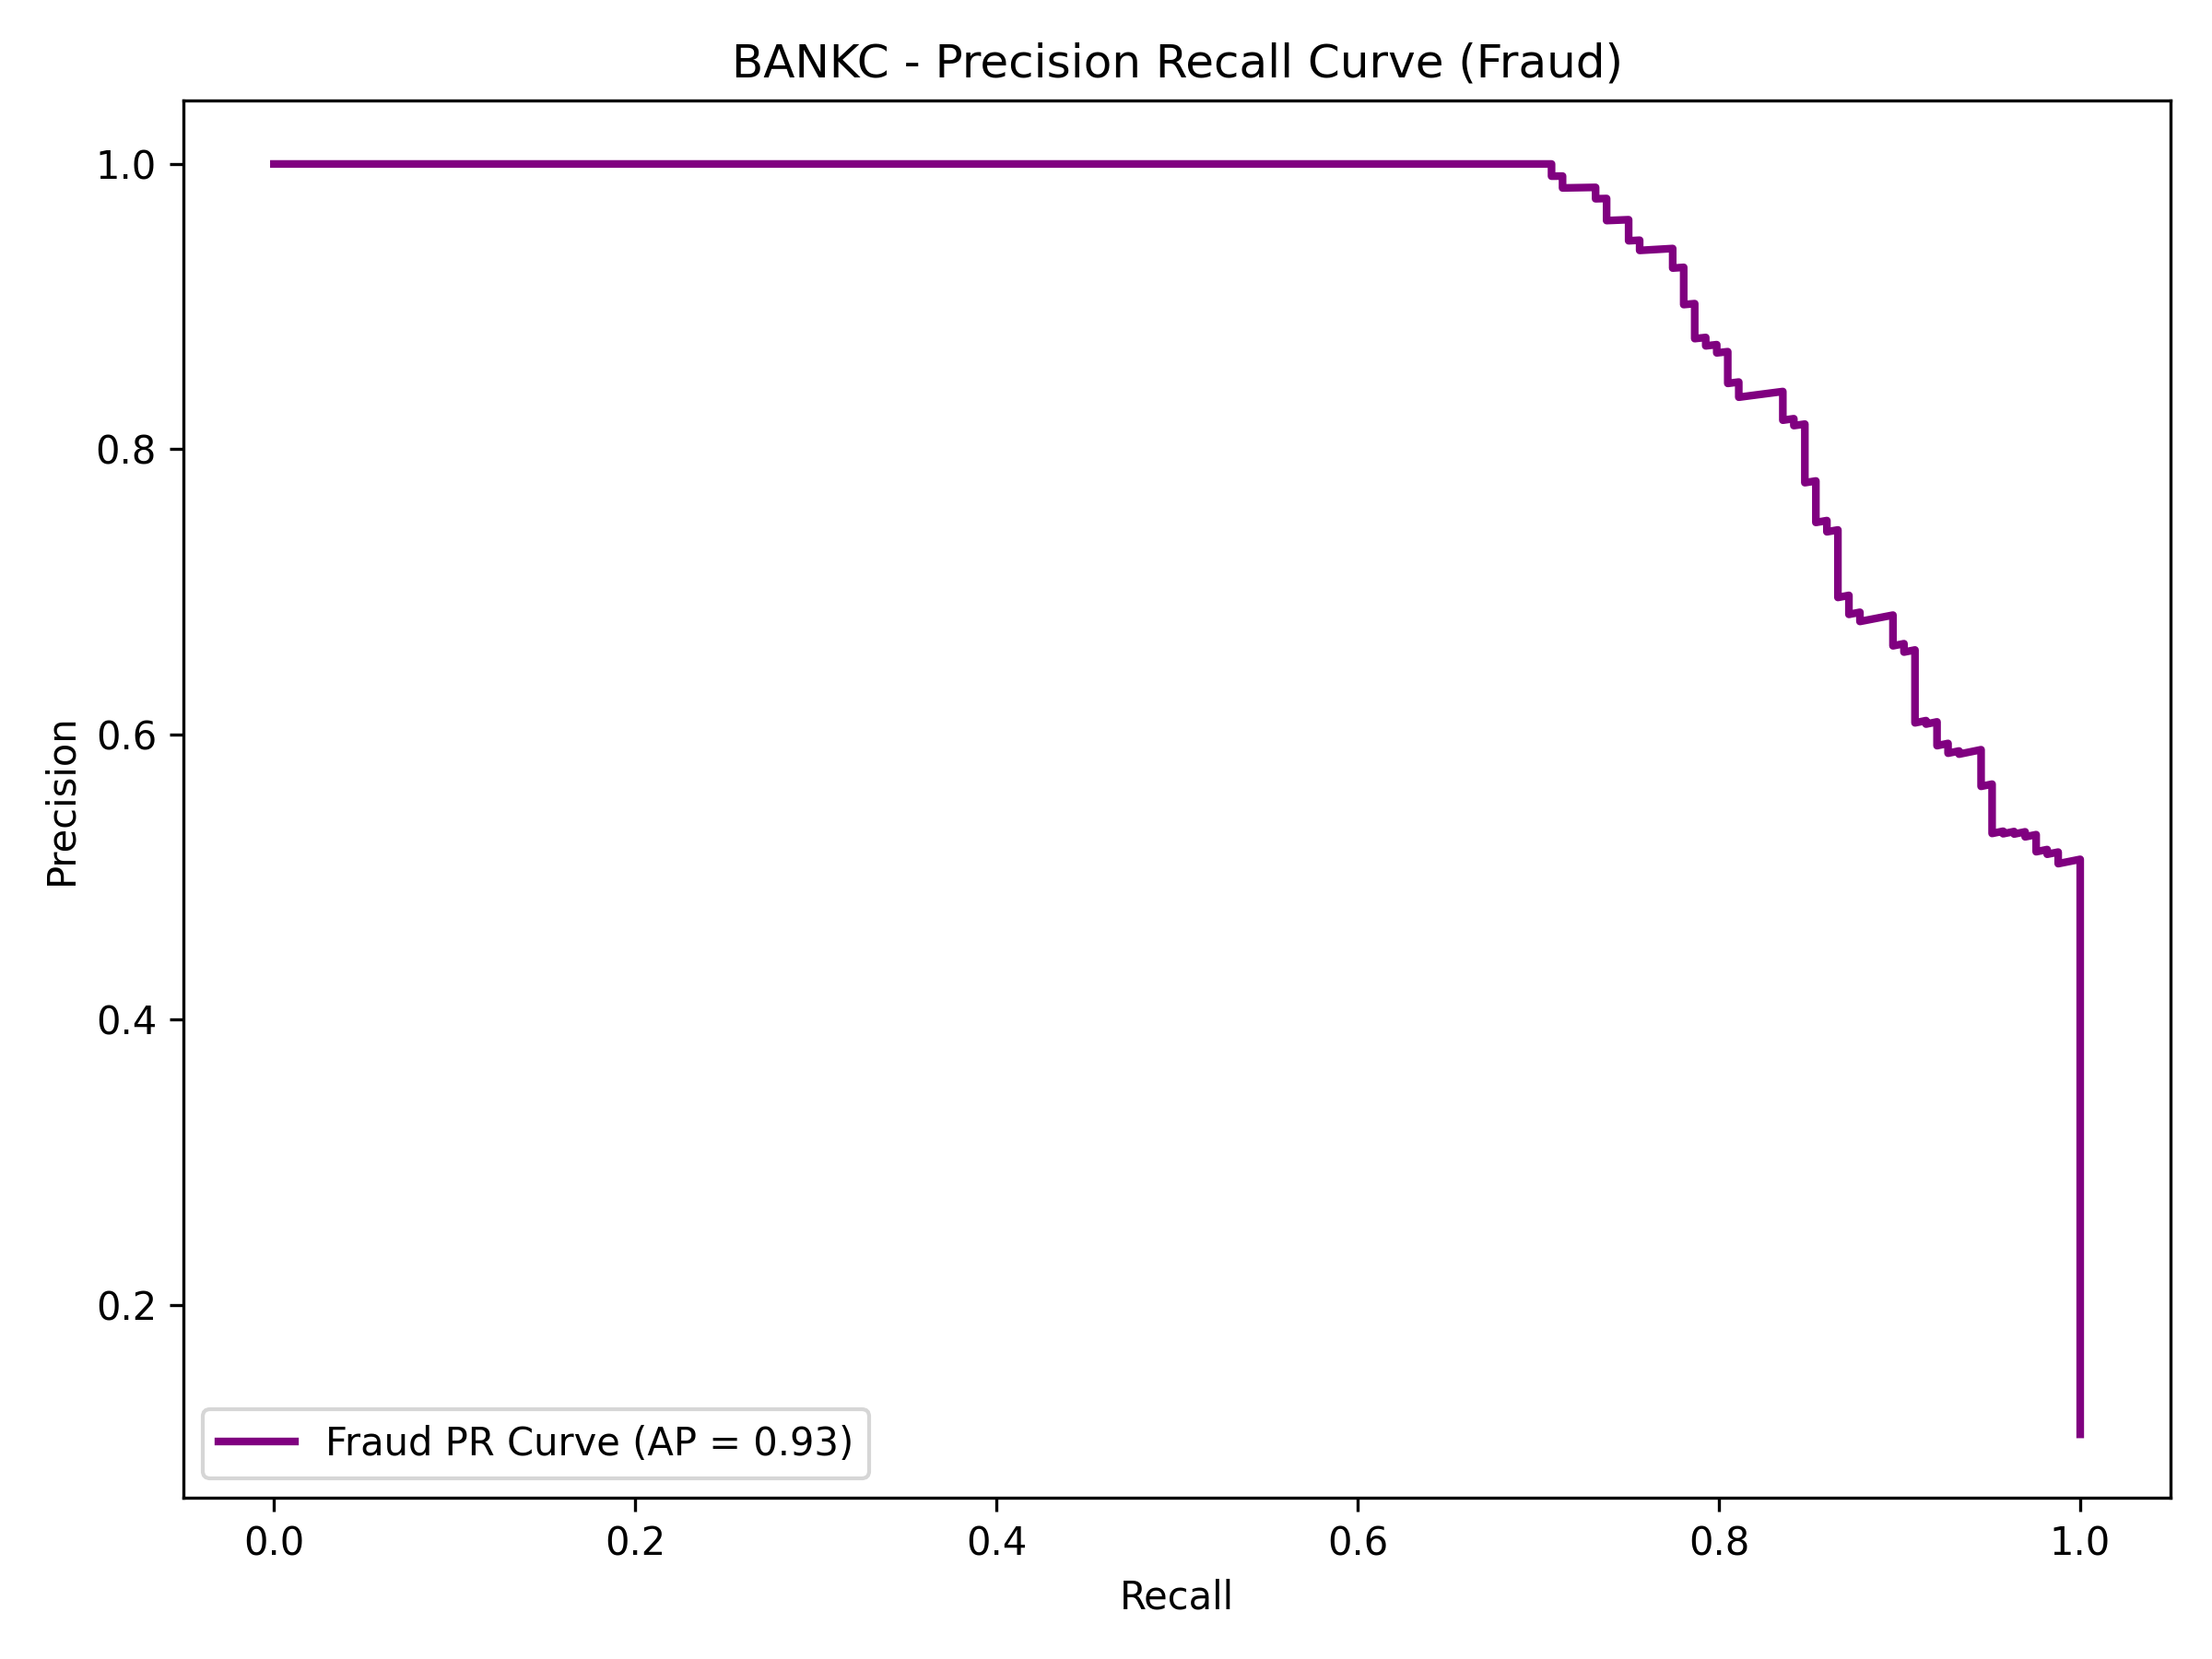
\includegraphics[width=\linewidth]{Figures/bankc_pr_curve_deep.png}
\end{minipage}
\hfill
\begin{minipage}{0.48\textwidth}
\centering
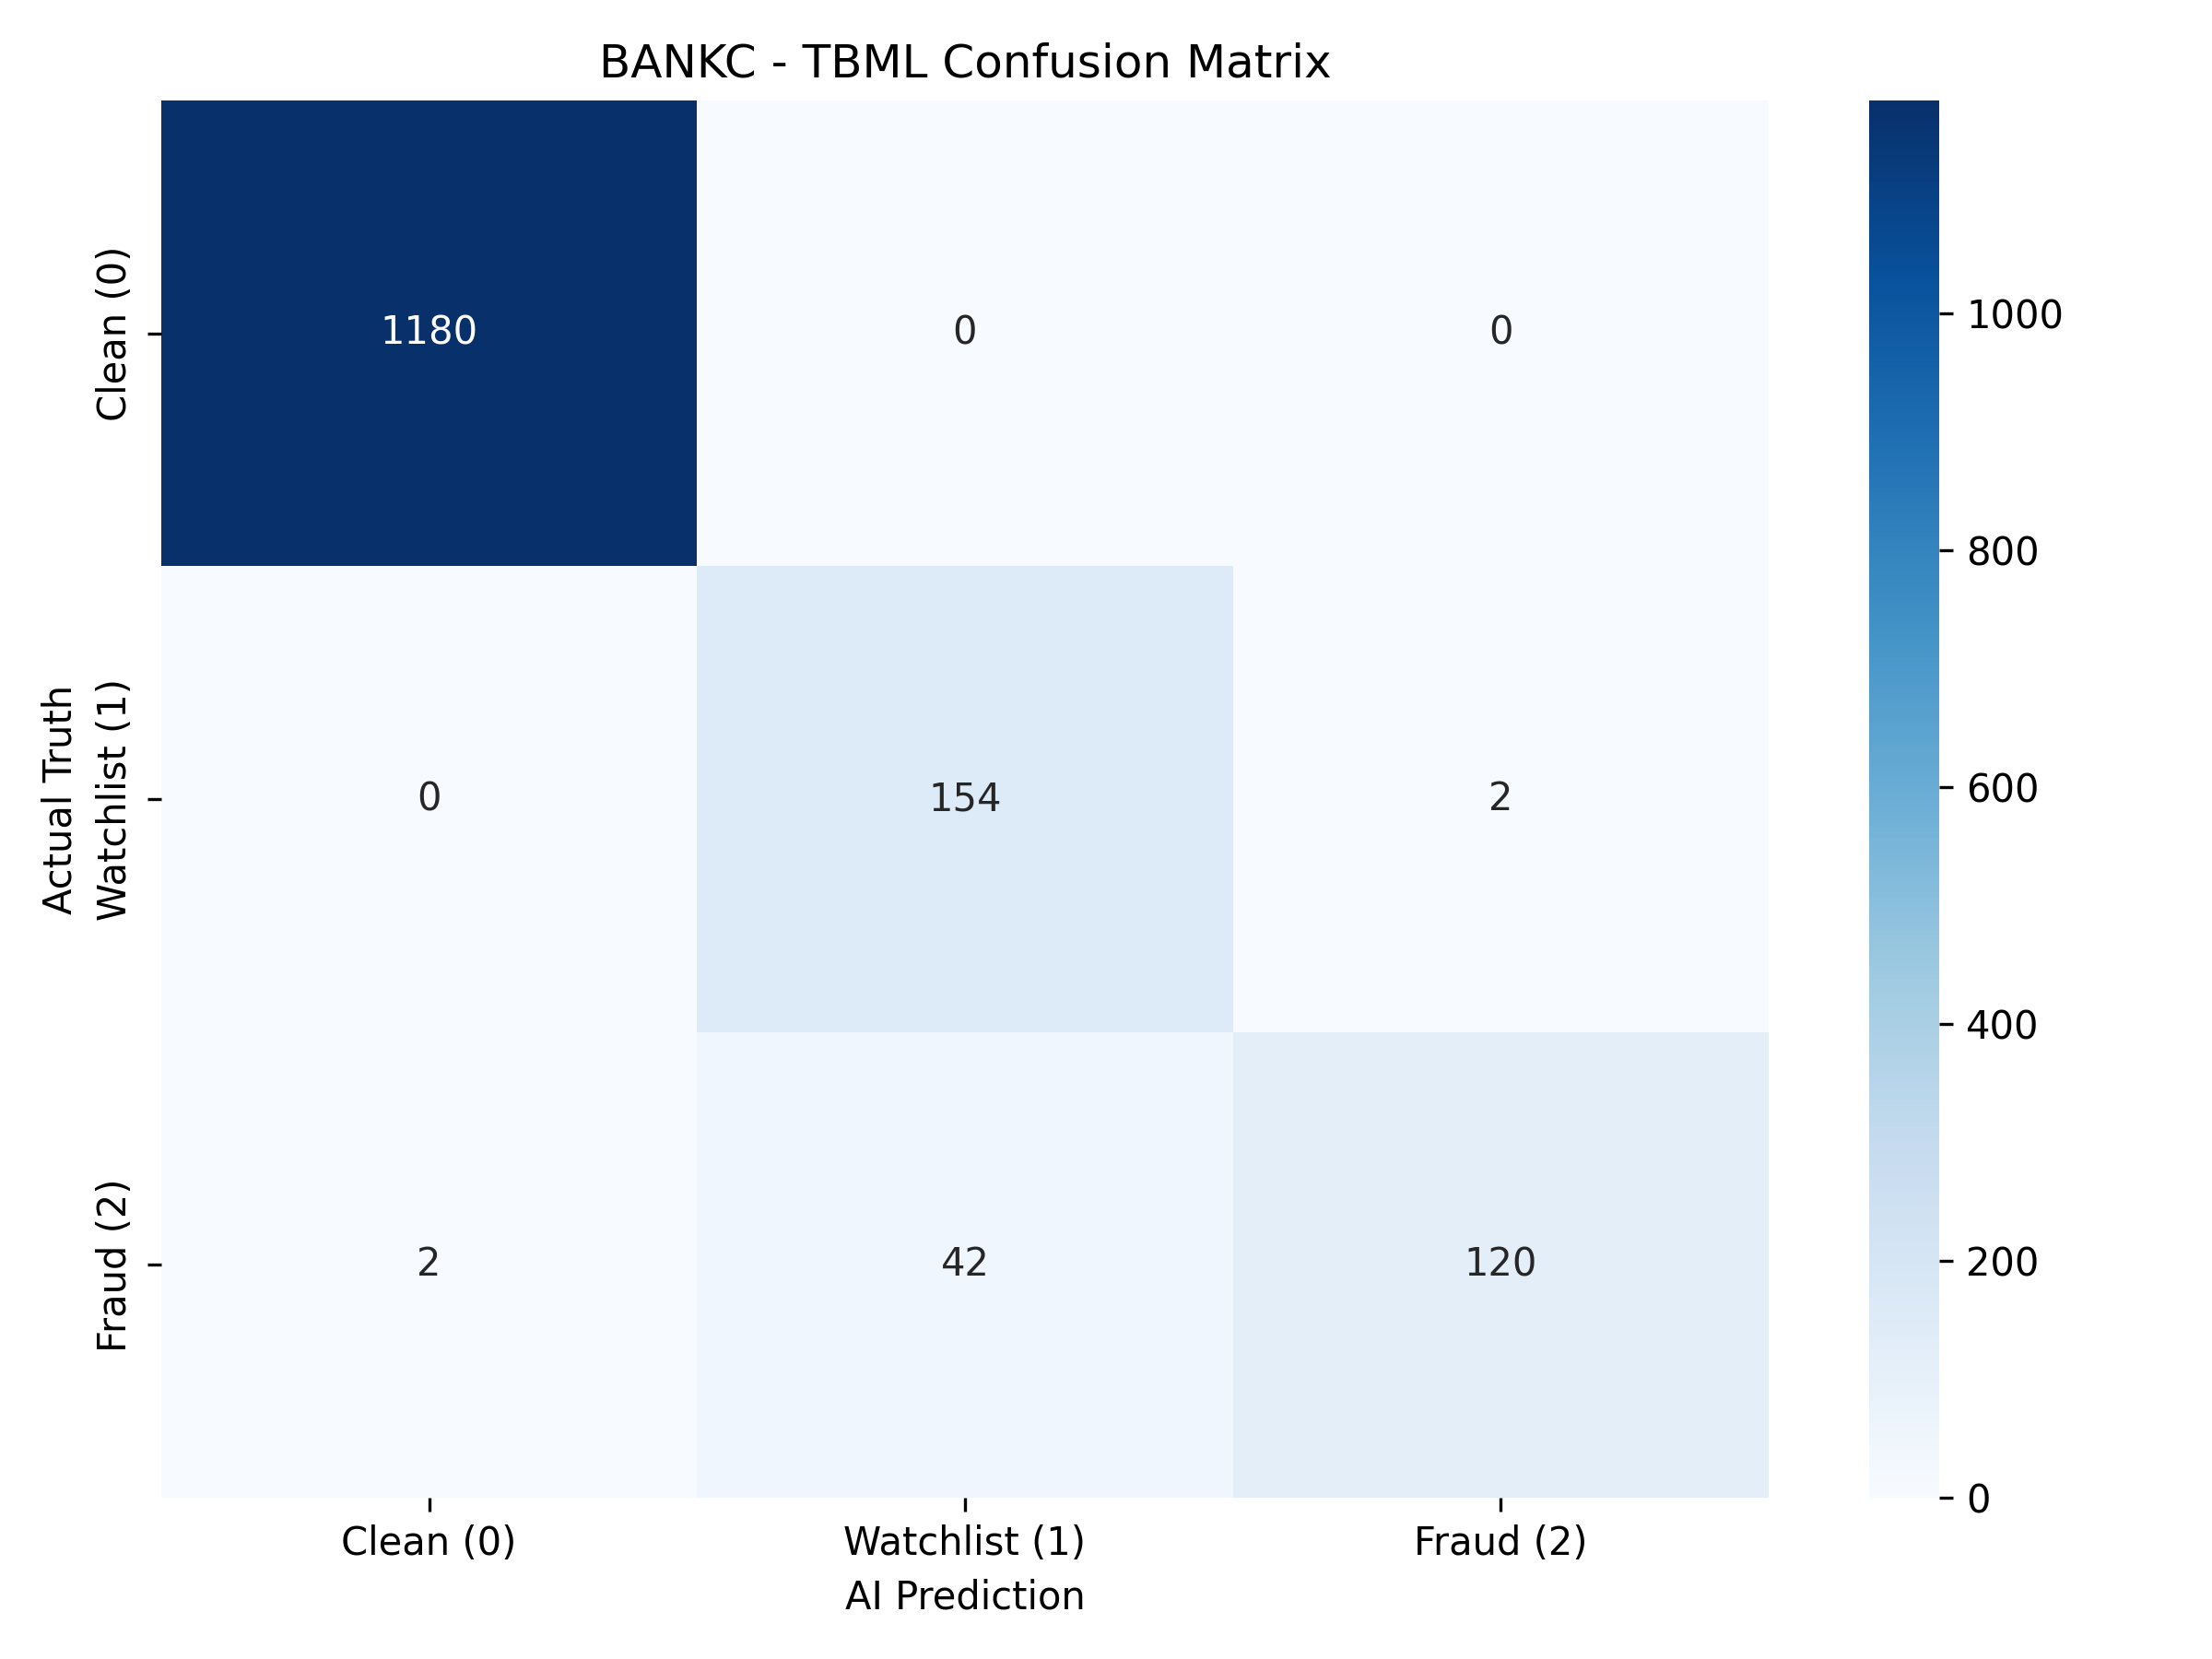
\includegraphics[width=\linewidth]{Figures/bankc_confusion_matrix_deep.png}
\end{minipage}

\caption{BANKC Precision--Recall Curve and Confusion Matrix Validation}
\label{fig:bankc_validation}
\end{figure}

As shown in Figure~\ref{fig:bankc_validation}, BANKC achieved similarly stable Precision--Recall performance, with Average Precision approaching 0.93. The curve remained steady even at higher recall levels, which points to dependable fraud detection under an imbalanced transaction distribution. The confusion matrix again showed strong consistency for legitimate transactions and very little false-positive spillover into the clean class. Most of the overlap stayed between Watchlist and Fraud, which confirms that the federated model generalized well across isolated institutional datasets.

%========================================================
\section{Summary}
%========================================================
The conducted testing and evaluation workflows validated the operational stability, synchronization reliability, and analytical performance of the proposed TBML detection framework across distributed institutional monitoring environments. The testing results confirmed stable backend communication, reliable transactional synchronization, controlled API response behavior, and successful workflow execution across graph-processing, federated analytical inference, dashboard synchronization, and compliance-management services. Concurrent scalability validation additionally demonstrated stable PostgreSQL query execution and controlled latency characteristics under increasing institutional workloads. The model performance evaluation further validated strong multi-class classification capability, stable federated convergence behavior, and reliable fraud-discrimination performance across heterogeneous institutional transaction environments without requiring centralized sharing of sensitive financial datasets.